\documentclass[11pt]{article}
 
\usepackage[letterpaper,portrait, margin=1in]{geometry}
\usepackage[parfill]{parskip}

\usepackage{graphicx}
\usepackage{amsmath,amsfonts,amsthm,amssymb}
\usepackage{epstopdf}
\usepackage{xcolor}
\usepackage{enumerate}
\usepackage{fancyhdr}
\usepackage{bigints}
\usepackage{setspace}
\usepackage{mathtools}
\usepackage{hyperref}
\usepackage{pifont}
\usepackage{todonotes}
\usepackage{setspace}
\usepackage{subfig}
\usepackage{float}
\usepackage{graphicx}
\usepackage{listings}
\usepackage{framed}
\usepackage{bbding}
\usepackage{fancyhdr}
\usepackage{color}
\usepackage{capt-of}
\usepackage{subfloat}
\usepackage{fixfoot,xspace}
\usepackage[inline]{enumitem}
\usepackage{subfig}
\usepackage{array}
\usepackage{multirow}
\usepackage{booktabs,caption,fixltx2e}
\usepackage[flushleft]{threeparttable}
\usepackage{lscape}
\usepackage{makecell}
\usepackage{amssymb}
\usepackage[mathscr]{euscript}
\usepackage{algorithm}
\usepackage{algpseudocode}
\usepackage{pifont}
\usepackage{caption}
\usepackage{algorithmicx}
\usepackage{hyperref}
\usepackage{mathrsfs}
\usepackage{tabularx}
\usepackage{bbm}
\urlstyle{same}
\usepackage{soul}
\usepackage{blindtext}
\usepackage{longtable}
\hypersetup{
colorlinks=true,
linkcolor=black,
citecolor=black,
filecolor=black,
urlcolor=black,
}

\usepackage{tikz}
\usetikzlibrary{shapes.geometric,shapes.multipart}
\usetikzlibrary{positioning}
\usetikzlibrary{decorations.pathreplacing}

\onehalfspacing
\renewcommand{\arraystretch}{1.5}
 
\usepackage[most]{tcolorbox}
\tcbset{textmarker/.style={%
 enhanced,
 parbox=false,boxrule=0mm,boxsep=0mm,arc=0mm,
 outer arc=0mm,left=6mm,right=3mm,top=7pt,bottom=7pt,
 toptitle=1mm,bottomtitle=1mm,oversize}}
\newtcolorbox{commentBox}{textmarker,
 borderline west={6pt}{0pt}{gray},
 colback=gray!10!white}

\newlist{todolist}{itemize}{2}
\setlist[todolist]{label=$\square$}
\usepackage{pifont}
\newcommand{\cmark}{\ding{51}}%
\newcommand{\xmark}{\ding{55}}%
\newcommand{\done}{\rlap{$\square$}{\raisebox{2pt}{\large\hspace{1pt}\cmark}}%
\hspace{-2.5pt}}
\newcommand{\wontfix}{\rlap{$\square$}{\large\hspace{1pt}\xmark}}
\DeclareMathOperator*{\argmax}{argmax}
\DeclareMathOperator*{\argmin}{argmin}
\DeclareMathOperator{\EX}{\mathbb{E}}% expected value

\makeatletter
\newcommand{\vast}{\bBigg@{4}}
\newcommand{\Vast}{\bBigg@{5}}
\makeatother

\usepackage{natbib}
 \bibpunct[, ]{(}{)}{,}{a}{}{,}
 \def\bibfont{\small}
 \def\bibsep{\smallskipamount}
 \def\bibhang{24pt}
 \def\newblock{\ }
 \def\BIBand{and}
 
\allowdisplaybreaks

\renewcommand{\algorithmicrequire}{\textbf{Input:}}
\renewcommand{\algorithmicensure}{\textbf{Output:}}

\usepackage[utf8]{inputenc}
\usepackage[english]{babel}
\usepackage{graphicx}

\newcommand*{\LargerCdot}{\raisebox{-0.25ex}{\scalebox{1.2}{$\cdot$}}}

\DeclareMathOperator{\Bern}{Bern}

%\setlength{\parskip}{0.4em}

\usepackage{lineno}
%\linenumbers 
\newtheorem{theorem}{Theorem}[] %%added for theorem
\newtheorem{stat}{Statistical Condition}[]
\newtheorem{corollary}{Corollary}[]
\newtheorem{remark}{Remark}[]
\newtheorem{lemma}{Lemma}[]
\newtheorem{proposition}{Proposition}[]
\newtheorem{definition}{Definition}[]
\newtheorem{assumption}{Assumption}[]

%%%%%%%%%%%%%%%%

\makeatletter
\DeclareFontFamily{U}{tipa}{}
\DeclareFontShape{U}{tipa}{m}{n}{<->tipa10}{}
\newcommand{\arc@char}{{\usefont{U}{tipa}{m}{n}\symbol{62}}}%

\newcommand{\arc}[1]{\mathpalette\arc@arc{#1}}

\newcommand{\arc@arcx}[2]{%
\sbox0{$\m@th#1#2$}%
\vbox{
\hbox{\resizebox{\wd0}{\height}{\arc@char}}
\nointerlineskip
\box0
}%
}
\makeatother

\input{abbrev}
 
\title{\bf\Large MS-DSC-2024-06576\\``Learning to cover: online learning and optimization with irreversible decisions''\\ Response to the reviewers and summary of improvements}
\author{}
\date{}

\begin{document}

\maketitle

We are pleased to resubmit for publication Manuscript MS-DSC-2024-06576. We are grateful for the feedback and the suggestions from the entire review team. This revision has significantly improved the manuscript by strengthening its methodological and practical contributions. Before responding to each comment, we first summarize the major improvements made over this revision.

\tableofcontents

\newpage

\section*{Overview of major improvements}
\addcontentsline{toc}{section}{\protect\numberline{}Overview of major improvements}%
\label{sec:overview}

\textbf{New statistical learning results.}

The main concern with the original submission was the assumption that the generalization error of the machine learning model decays to 0 with the square root of the sample size.
\begin{assumption}[Original manuscript] \label{ass:classification_old_summary}
    There exists $0<\varepsilon\leq 1$ such that the error of the machine learning model $f_t$ trained with $N_{t-1}$ samples is bounded by:
    \begin{align*}
         \P_{t}(f_t(\bx_{it})\neq S_{it})\leq \frac{\varepsilon }{\sqrt{N_{t-1} + 1}}.
    \end{align*}
\end{assumption}

We had justified this assumption from statistical learning theory. However, this suffered from two limitations: (i) the data samples are not independent in our online learning and optimization environment, and (ii) the machine learning model may predict the distribution of facility success rather than its true realization. We have completely overhauled this assumption: rather than \textit{positing} the form of the learning error, we now \textit{prove} that, under certain statistical conditions, our learning process converges to the optimal Bayes classifier at a rate of at best $\calO(1/\sqrt{n})$.
\begin{proposition}[Revised manuscript, informal]\label{prop:MLE_informal_summary}
       Under statistical learning conditions, the error rate of the learned classifier, denoted by $\mu_t$ converges to that of the Bayes-optimal classifier, denoted by $\mu^*$, as follows, for some $\alpha>0$, for any $\varepsilon,\gamma>0$, and for $N_{t-1}$ large enough:
        \[\mu_t \leq \frac{\overline\varepsilon}{(N_{t-1}+1)^{\min\{\alpha,1\}\times (1/2-\gamma)}}+\mu^*.\]
\end{proposition}

The newly-added Section 3 in the revised manuscript defines a formal statistical learning environment to establish rigorously the convergence properties of the online classifier. This includes:
\begin{itemize}[topsep=-2pt,itemsep=-2pt]
\item[--] \emph{Clarifications on the probabilistic environment.} We have formalized the randomness in facility success: each facility $i\in\calF$ is associated with a ``true'' (unknown) probability of success $\eta_{i}$, and facility success, denoted by $S_{it}$, follows independent Bernoulli trials.
\item[--] \emph{A new statistical learning environment.} We define a new statistical learning setting in which the model learns the \textit{distribution}, that is, the probabilities of success $\eta_{it}$, rather than the \textit{realizations} $S_{it}$. The online learning and optimization setting accounts for residual error.
\item[--] \emph{Non-i.i.d. samples.} We have formalized the online learning and optimization problem to underscore the interdependence between data samples. The learning model in period $t$ impacts the decisions in period $t$, which impact the sample and learning model in period $t+1$, etc. Over time, the sample becomes increasingly biased toward high-probability realizations.
\item[--] \emph{A new statistical learning result.} We prove that, under certain statistical conditions, the online classifier converges to the optimal Bayes classifier at a rate of at best $\calO(1/\sqrt{n})$, as outlined in Proposition~\ref{prop:MLE_informal_summary} above. Notably, the online classifier learns the distribution of the uncertain parameters rather than the realizations themselves.
\item[--] \emph{Rigorously formulating the online learning and optimization problem.} We leverage our statistical result to model, conservatively, facility success via the upper-bounding error rate, and show that the number of successful facilities follows a binomial distribution at each time period. This completes the bridge from our problem statement to its mathematical formulation.
\end{itemize}

\textbf{New online learning and optimization results.}

\begin{itemize}[topsep=-2pt,itemsep=-2pt]
\item[--] \emph{A more general problem formulation.} Based on Proposition~\ref{prop:MLE_informal_summary}, we consider a generic learning function with a learning rate $\calO(1/n^r)$ (which generalizes the best-case rate of $\calO(\sqrt n)$ to classification settings) and an irreducible error term $1-p$ (which captures the Bayes error).
\item[--] \emph{Updates to our algorithm and our regret bounds.} We have extended our theoretical analysis to account for instances with a residual error ($p<1$) and different learning rates ($r\neq0.5$). For all learning functions, we obtain asymptotically-tight sub-linear regret bound up to the second-leading order with a constructive algorithm, both in the core and the networked problems.
\item[--] \emph{New proof techniques.} In the core problem, we have replaced Hoeffding's inequality with Bernstein's inequality and the Berry-Esseen theorem to derive matching lower and upper bounds up to the second-leading order across all learning regimes. In the networked problem, we have replaced the concentration inequality from \cite{janson2004large} by the recent result from \cite{janisch2024berry}, which extends the Berry-Esseen theorem in dependency graphs.
\end{itemize}

\textbf{Extensions: static vs. adaptive decision-making.}

\begin{itemize}[topsep=-2pt,itemsep=-2pt]
\item[--] \emph{A new theoretical result showing limited benefits of adaptiveness.} We prove that an adaptive re-optimization algorithm leads to the same asymptotic rates of facility openings and the same asymptotic regret rate for the first $T-1$ periods as the offline, static algorithm. This result yields a surprising insight on the limited benefits of adaptiveness in our online problem.
\item[--] \emph{An interpretable semi-adaptive algorithm.} We have proposed a ``semi-adaptive'' approach that relies on the static solution for the first $T-1$ periods and a final-period adjustment to \textit{exactly} satisfy the chance constraint (without the buffer from our theoretical algorithm). New computational results show the strong performance of this simple and interpretable algorithm.
\end{itemize}

\textbf{Other improvements.}

\begin{itemize}[topsep=-2pt,itemsep=-2pt]
\item[--] \emph{New computational experiments.} We have applied our online learning and optimization methodology to four datasets from the \cite{UCI}. Newly-added results show that our statistical learning assumption---derived from our new statistical result despite the lack of independence across samples---provides a good approximation of out-of-sample performance. Moreover, they show that the proposed online and optimization procedure leads to significant performance improvements over the no-learning baseline.
\item[--] \emph{Enhanced computational results.} We also show that our (theoretical) algorithm provides a good approximation of the chance-constrained problem. The results strengthens the discussion of the trade-off between limited exploration and full-scale exploitation.
\item[--] \emph{Revised exposition.} We have improved the writing to provide more intuition. In particular, we have added several figures to make the arguments more visual. We have also clarified that our algorithms rely on a deterministic approximation plus a coverage buffer to account for uncertainty in facility success, and provided more insights into the proof techniques.
\end{itemize}

\textbf{Stronger statement of contributions.}\

This revision has considerably elevated the quality of the paper, its statistical grounding, and its technical depth. Notably, the revised manuscript provides an end-to-end approach to a new class of online learning and optimization problems, as stated in the new summary of contributions:
\begin{quote}
    ``This paper develops a new end-to-end framework for dynamic decision-making under uncertainty, where each action simultaneously advance a strategic coverage objective and generate informative data for future decisions. We formalize this setting as a novel class of coupled online learning and optimization environments. First, we provide theoretical guarantees on the convergence of the online classifier in this environment to the Bayes-optimal classifier. We then leverage these insights to develop a tractable optimization formulation of the online learning and optimization problem. We derive tight upper and lower bounds the regret rates up to the second-leading order. Finally, we design a practical, interpretable policy and prove its asymptotic feasibility and optimality up to the second leading order. The structure of the policy, featuring limited initial exploration followed by rapid exploitation, highlights the tangible benefits of structured pilot deployments in strategic planning under uncertainty. We also show that this structure is robust to offline data, different learning functions, and adaptive decision-making. Together, these contributions offer a unified theoretical and algorithmic foundation for planning under learning uncertainty, blending tools from statistical learning, online optimization, and decision theory.''
\end{quote}

\textbf{Extensions left for future research.}

We also acknowledge two suggestions left for future research, discussed in the conclusion.

\begin{itemize}[topsep=-2pt,itemsep=-2pt]
\item[--] \emph{Finite-sample analysis.} Our paper defines and studies a new asymptotic regime with an infinitely large coverage target but a limited planning horizon. An extension would be to leverage finite-sample concentration inequalities to extend our results to a setting with a finite coverage target, or to the networked setting without our degree assumption.
\item[--] \emph{An enhanced heuristic algorithm in the networked setting.} Our (theoretical) algorithm relies on a discrete non-linear optimization formulation. We solve it via a (computational) algorithm that is optimal in star graphs and a principled heuristic in general. This could be extended with more involved algorithms to ensure exactness in general graphs.
\end{itemize}

\newpage

\newpage
\section*{Response to the Department Editor's Comments}
\addcontentsline{toc}{section}{\protect\numberline{}Response to the Department Editor's Comments}

\begin{commentBox}

The review team unanimously finds the problem setting as well as the proposed solution intriguing, but they have a number of major concerns. They believe that these concerns may well be addressable, but that the work involved extends beyond what would commonly be considered a major revision. As a result, the associate editor suggests a rejection with the possibility to resubmit the manuscript.

Although Management Science aims to move away from those ``reject-and-resubmit's'', I believe this work deserves the option to be reconsidered. I agree with the review team that the manuscript shows quite some promise, and I hope that the concerns of the review team can be addressed in a convincing way. I would therefore welcome a resubmission of the manuscript to Management Science. If you decide to do so, please attach a point-by-point response to the comments raised and clearly state in the cover letter that it is a resubmission so that it can be routed back to the same review team.
\end{commentBox}

Thank you for leading the review process and for synthesizing the comments from the Associate Editor and the two reviewers. We appreciate your encouraging comments on the problem setting, the solution approach, and the theoretical results. We also understand the concerns regarding the problem statement, its mathematical formulation, and some of our technical results. All reports were thorough and constructive, and offered excellent suggestions to strengthen our theoretical, methodological and practical contributions. We are also grateful for your supportive recommendation defining a path forward and inviting a resubmission.

As you can see throughout this response document, we have closely followed the suggestions to revise the paper. First and foremost, we have added a new section at the outset of the paper to establish rigorous statistical learning results in our online learning and optimization environment. The original manuscript was \textit{positing} from statistical learning theory that the generalization error rate decays to 0 with the square root of the sample size. However, the reviewers rightly pointed out that standard results could not be readily applied because of the lack of independent and identically distributed samples and because individual realizations may not be perfectly learnable from the features. Instead, the revised manuscript \textit{proves} that, under certain statistical conditions, our learning process converges to the optimal Bayes classifier at a rate of at best $\calO(1/\sqrt{n})$; notably, the online classifier learns the distribution of the uncertain parameters rather than the realizations themselves. This result provides one instantiation—rather than a unique characterization—of statistical conditions with these convergence properties; we then abstract away from this particular setup to formulate a general statistical learning function characterized by an initial error $\varepsilon$, a learning rate of order $\calO(1/n^{r})$, and an irreducible-error share of $1-p$; and we rigorously characterize the number of successful facilities via a binomial distribution under this statistical setting. This newly-added section provides necessary theoretical grounding to bridge our problem statement and the mathematical formulation, thereby enhancing the quality and rigor of the manuscript.

We have also updated all results and proof techniques throughout the paper to accommodate the residual Bayes error rate and generic rates of convergence. This more general learning environment required extensions of our main results and new proof techniques. Specifically, when the Bayes error rate is zero, we prove tight regret bounds in $\Theta\left(m^{\frac{1-r}{1-r^T}}\right)$, where $r\neq1$ denotes the learning rate (extending the results from our original submission to $r\neq0.5$); otherwise, we prove tight regret bounds in $\Theta\left(\max\left\{m^{\frac{1-r}{1-r^T}},\sqrt{m}\right\}\right)$, where the $\sqrt{m}$ regret comes from the non-zero residual learning error. In both cases, we have upgraded our algorithm design and our proof techniques to ensure matching rates in our lower-bounding analysis of the optimal solution and our upper-bounding analysis of our algorithm's solution across all learning regimes, notably by replacing Hoeffding's inequality with the Berry-Esseen theorem and with Bernstein's inequality, and by replacing the concentration inequality in dependency graphs from \cite{janson2004large} by the one from \cite{janisch2024berry}.

We have added extensions to compare the algorithm's solution to the exact solution of the problem in small-enough samples, and to compare our (static) algorithm to adaptive re-optimization procedures. In particular, we have derived new theoretical results that show that the static algorithm and an adaptive re-optimization approach achieve the same asymptotic rates of facility openings and the same asymptotic regret rate for the first $T-1$ periods; this result suggest limited benefits of adaptivity and therefore uncovers the strength of the static optimization problem considered in the paper. In addition, new computational results show the strong performance of a simple and interpretable semi-adaptive algorithm, combining the static solution for the first $T-1$ periods and a simple final-period adjustment to exactly meet the chance constraint.

Finally, we have conducted new computational experiments to showcase our online learning and optimization in action, using four datasets from the \cite{UCI}. We first show that our learning assumption---derived from our new statistical result despite the lack of independence across samples---provides a good approximation of out-of-sample performance. We then demonstrate that our online and optimization algorithm leads to strong performance improvements over the no-learning baseline. This extension have strengthened the practical impact of the paper by showing its benefits using real-world data and data-driven machine learning models.

In turn, the paper provides a true end-to-end approach to a new class of online and optimization problems. We begin by formalizing the online learning environment and proving that the error rate admits a precise upper bound with a specific functional form. Building on this foundation, we formulate a rigorous mathematical model, derive tight asymptotic lower and upper bounds up to the second-leading order, and develop a tractable and interpretable algorithm that yields an asymptotically-feasible and asymptotically-optimal solution. We show that the main insights are robust to different learning rates, different levels of irreducible error, offline data, and adaptive solution strategies. We then extend the full framework to a graph-based setting; despite a much more complex structure, we prove analogous results and develop a new deterministic algorithm with similar asymptotic guarantees. Finally, we validate the approach on synthetic data and on real-world data from the \cite{UCI}, providing evidence of both the quality of our statistical learning approximation and of the the practical benefits of our online learning and optimization algorithm. Together, these results offer a complete theoretical, algorithmic, and empirical foundation for a new class of online learning and optimization problems.

For details, see the \hyperref[sec:overview]{\color{blue}overview of major improvements}. We believe that it has made every aspect of our manuscript significantly stronger. We hope that the new version will address the concerns from the review team. We look forward to your editorial decision on the new version of the manuscript.

\newpage
\section*{Response to the Associate Editor's Comments}
\addcontentsline{toc}{section}{\protect\numberline{}Response to the Associate Editor's Comments}

\begin{commentBox}
\textbf{Comment 1.}\label{AE:1}

This paper proposes a suite of algorithms for a covering problem that incorporates learning and optimization, where a decision maker must cover demand with some service rate by opening covering facilities sequentially, while minimizing the number of opening attempts. As the DM opens facilities they gain information that allows to better predict the success likelihood of future facilities to open. There is thus an exploration-exploitation trade-off between opening enough facilities to learn, versus paying the cost of another opening.

The authors present an algorithm for this problem with provable regret guarantees in the scaling where the number of facilities is large, but the number of decision points (time horizon) is finite, which is a novel regime that diverges from the more conventional learning literature. They then define a version of their coverage problem in a bipartite graph, where each facility can only serve a subset of customers. They present a generalization of the baseline algorithm which attains similar regret bounds under certain assumptions on the connectivity of the underlying graph, and assuming an exact solution to a non-linear integer optimization problem. Finally, they present a heuristic to solve the aforementioned problem efficiently.

These models are applicable to clinical trials, retail stores, and energy infrastructure deployment.
\end{commentBox}

Thank you for the detailed summary of our paper. Your synthesis highlights the main characteristics of our setting (online learning and optimization with irreversible decisions contributing toward a coverage target), the two decision-making environments (a core setting with a supply-side target on facilities and a networked setting with a demand-side target on customers), the novel asymptotic regime (an asymptotically large coverage target but a finite time horizon), and the practical motivating examples (clinical trials, retail stores, and infrastructure planning). As you also noted, we derive tight upper and lower bounds with guarantees of asymptotic feasibility and asymptotic optimality, and we propose constructive algorithms that generate an asymptotically feasible and asymptotically optimal solutions up to the second-leading order. Our results uncover a sublinear learning rate that decays exponentially as the time horizon gets longer, thereby yielding novel managerial insights on the benefits of even limited online learning and optimization.

\begin{commentBox}
\textbf{Comment 2.}\label{AE:2}

I sent the paper out to three expert reviewers, who I thank for their careful feedback. For reference, R1’s review starts with ``This paper considers the problem faced by a decision-maker who needs to cover demand by sequentially opening new facilities.'' R2’s starts with ``This paper presents an online learning and optimization framework for a facility location selection problem, where decisions are irreversible'' and R3’s with ``The core contribution of the paper lies in developing an optimal algorithm that balances the trade-off''.
\end{commentBox}

Thank you for leading the review process. We appreciate the detailed reports from the three reviewers. The comments were balanced, fair and constructive. We have endeavored an extensive revision of the paper to address their concerns. In particular, we have added an entire new section to the paper that develops a statistical learning framework for our problem, extended all our results to new learning regimes accordingly, established the robustness of our approach against adaptive decision-making policies, and demonstrated the practical benefits of our approach on real-world datasets. The revised manuscript is undoubtedly stronger as a result.

\begin{commentBox}
\textbf{Comment 3.}\label{AE:3}

All referees are positive about the general motivation and contribution of the paper. To quote R1,
\begin{quote}
    The research question is practically relevant, and the problem formulation is quite elegant. In particular, the authors’ emphasis on a small number of sequential decisions (small $T$) deviates from the classical perspective adopted in online learning.
\end{quote}
I must say I agree – the problem is interesting, quite well motivated, and with a sound technical contribution behind it.

\end{commentBox}

We appreciate the positive comments from the entire review team on the problem statement, the practical motivations, our technical contributions, and their managerial implications. We have aimed to maintain the strength of these contributions in the revised manuscript, while broadening the scope of the paper, deriving new results, and clarifying its takeaways.

\begin{commentBox}
\textbf{Comment 4.}\label{AE:4}

At the same time, the referees also question some of the assumptions of the paper, mostly around the model for learning under uncertainty, and again I fully agree with them. At the core, the formulation of the problem is currently confusing and potentially unrigorous – please see my first major comment below (as well as the referee reports) for what I view as the main pain-point of the paper. While I suspect these issues can be tackled while salvaging the key algorithmic contributions of the paper, they are serious and probably require rewriting that goes beyond one round of major revision. I must therefore recommend rejection. However, I believe the core ideas in this paper are worthwhile, I would welcome a resubmission should the authors address these concerns, and I would enjoy reading it.

I’m sorry I cannot have better news, but I do hope that the editorial comments will be useful for the authors to improve their paper.
\end{commentBox}

We appreciate the concerns from the review team, which helped us strengthen the contributions of the paper. As you highlighted, the main pain-point lied in the core assumptions on the learning environment, and the lack of clarity underlying the mathematical formulation of the online learning and optimization problem as a result. We are grateful for your encouraging view that the issues can be addressed and for inviting a resubmission. We have closely followed your suggestions on a path forward, and have comprehensively revised the manuscript to address the concerns.

In response to the main pain-point that you identified, we have added a new section (Section 3) that establishes the validity of the online learning and optimization formulation. This section defines a rigorous statistical learning framework, and proves the convergence properties of the online classifier. The original manuscript was \textit{positing} from statistical learning theory that the generalization error rate decays to 0 with the square root of the sample size. However, the reviewers rightly pointed out that standard results could not be readily applied because of the lack of independent and identically distributed samples and because individual realizations may not be perfectly learnable from the features. Instead, the revised manuscript \textit{proves} that, under certain statistical conditions, our learning process converges to the optimal Bayes classifier at a rate of at best $\calO(1/\sqrt{n})$; notably, the online classifier learns the distribution of the uncertain parameters rather than the realizations themselves. This result provides one instantiation—rather than a unique characterization—of statistical conditions with these convergence properties; we then abstract away from this particular setup to formulate a general statistical learning function characterized by an initial error $\varepsilon$, a learning rate of order $\calO(1/n^{r})$, and an irreducible-error share of $1-p$; and we rigorously characterize the number of successful facilities via a binomial distribution under this statistical setting. This newly-added section provides necessary theoretical grounding to bridge our problem statement and the mathematical formulation, thereby enhancing the quality and rigor of the manuscript.

We have also updated all results and proof techniques throughout the paper to accommodate the residual Bayes error rate and generic rates of convergence. This more general learning environment required extensions of our main results and new proof techniques. Specifically, when the Bayes error rate is zero, we prove tight regret bounds in $\Theta\left(m^{\frac{1-r}{1-r^T}}\right)$, where $r\neq1$ denotes the learning rate (extending the results from our original submission to $r\neq0.5$); otherwise, we prove tight regret bounds in $\Theta\left(\max\left\{m^{\frac{1-r}{1-r^T}},\sqrt{m}\right\}\right)$, where the $\sqrt{m}$ regret comes from the non-zero residual learning error. In both cases, we have upgraded our algorithm design and our proof techniques to ensure matching rates in our lower-bounding analysis of the optimal solution and our upper-bounding analysis of our algorithm's solution across all learning regimes, notably by replacing Hoeffding's inequality with the Berry-Esseen theorem and with Bernstein's inequality, and by replacing the concentration inequality in dependency graphs from \cite{janson2004large} by the one from \cite{janisch2024berry}.

We have added extensions to compare the algorithm's solution to the exact solution of the problem in small-enough samples, and to compare our (static) algorithm to adaptive re-optimization procedures. In particular, we have derived new theoretical results that show that the static algorithm and an adaptive re-optimization approach achieve the same asymptotic rates of facility openings and the same asymptotic regret rate for the first $T-1$ periods; this result suggest limited benefits of adaptivity and therefore uncovers the strength of the static optimization problem considered in the paper. In addition, new computational results show the strong performance of a simple and interpretable semi-adaptive algorithm, combining the static solution for the first $T-1$ periods and a simple final-period adjustment to exactly meet the chance constraint.

Finally, we have conducted new computational experiments to showcase our online learning and optimization in action, using four datasets from the \cite{UCI}. We first show that our learning assumption---derived from our new statistical result despite the lack of independence across samples---provides a good approximation of out-of-sample performance. We then demonstrate that our online and optimization algorithm leads to strong performance improvements over the no-learning baseline. This extension have strengthened the practical impact of the paper by showing its benefits using real-world data and data-driven machine learning models.

In turn, the paper provides a true end-to-end approach to a new class of online and optimization problems. We begin by formalizing the online learning environment and proving that the error rate admits a precise upper bound with a specific functional form. Building on this foundation, we formulate a rigorous mathematical model, derive tight asymptotic lower and upper bounds up to the second-leading order, and develop a tractable and interpretable algorithm that yields an asymptotically-feasible and asymptotically-optimal solution. We show that the main insights are robust to different learning rates, different levels of irreducible error, offline data, and adaptive solution strategies. We then extend the full framework to a graph-based setting; despite a much more complex structure, we prove analogous results and develop a new deterministic algorithm with similar asymptotic guarantees. Finally, we validate the approach on synthetic data and on real-world data from the \cite{UCI}, providing evidence of both the quality of our statistical learning approximation and of the the practical benefits of our online learning and optimization algorithm. Together, these results offer a complete theoretical, algorithmic, and empirical foundation for a new class of online learning and optimization problems.

As a result, the revised manuscript is much stronger, more rigorous and more comprehensive. The new submission also includes several other improvements in response to the reviewers' comments, as detailed in the \hyperref[sec:overview]{\color{blue}overview of major improvements} and throughout this document. Again, we are grateful for the opportunity to resubmit and we hope that it will address the concerns.

\begin{commentBox}
\textbf{Comment 5. Major comments: Uncertainty model.}\label{AE:5}

All referees point out serious issues with the uncertainty model that leads to the formulation $\calP^*$. I appreciate the intent to write the paper using a black-box estimation model for the likelihood of successful facility opening, but I think this sweeps a lot of important details under the rug and has lead to a lot of confusion. The authors should respond to all the relevant questions of the referees, but let me zoom in on a couple of points:

(a) R1 and R2 both point out that it’s not clear the re-formulation of $\calP^*$ from page 10 is correct. R2, and R1 implicitly, question why the chance constraint seems to be taken over the ML model’s predictions instead of the actual chance of success $v_{it}$. I also found this puzzling, and at the heart of this lies the fact that the authors do not actually define the randomness of $v_{it}$. I take it their intent was to have the model as general as possible, but without a rigorous bridge from that to the ML estimate and the re-formulated chance constraint, it does not currently make sense to me.

(b) There is an additional issue with the re-formulated chance constraint, again picked up by both R1 and R2. To cite R1
\begin{quote}
    ...the authors ultimately analyze the problem described on page 10, in which the success probability of selected facilities converges to 1. A more realistic assumption would be that the decision-maker learns the distribution (as opposed to the realizations) of $\bv$—i.e., facilities have different success probabilities, and as the number of samples grows, the ML model learns the success probability...
\end{quote}
Indeed, I am not sure how to interpret that chance constraint. Is the idea that ultimately you will have almost perfect predictors of success, so you will pick only the candidates for which the estimate of $v_{it} = 1$? Where in the model are we guaranteed this is even feasible, i.e. that there are enough ``good'' facilities to meet the opening target? Either case, this seems unrealistic, and at the minimum, needs to be properly explained in the paper.

(c) The referees also point out that typically to get any meaningful estimate (see Assumption 1), one needs to assume some form of independence of the samples used for estimation. But here the samples come out of running a stateful algorithm. There is no guarantee of independence, and I do not see why one should expect to construct a good estimator from the samples it collects along the way, which would yield either Assumption 1 in its current form, or a weaker version of it.

Unfortunately, these are critical issues, raised uniformly by the review team, that need to be unequivocally resolved quite carefully for the paper to make progress.
\end{commentBox}

Thank you for the detailed summary of the reviewers' concerns and for sharing your own thoughts on the learning environment. We appreciate your positive comment on the generalizability of our mathematical formulation, which indeed does not rely on any parametric assumptions regarding the machine learning model; however, our original manuscript was indeed too elusive on the statistical learning environment. As you mentioned in your previous comment, this is the most critical issue raised by the review team. We have addressed it fully in this revision by adding a new section at the outset of the paper (Section 3) that defines a rigorous probabilistic environment and that establishes the convergence of the classifier in our online learning and optimization environment.

We emphasize that this construction serves as one instantiation—rather than a unique characterization—of statistical conditions under which these convergence properties would hold. Importantly, these statistical conditions solely support the convergence assumption of the classifier and are not invoked in the derivation of our regret bounds and other results in the online learning and optimization problem.

Specifically, the original manuscript relied on the following statistical learning assumption, which stated that the generalization error decays to 0 with the square root of the sample size.
\setcounter{assumption}{0}
\begin{assumption}[Original manuscript] \label{ass:classification_old_AE}
    There exists $0<\varepsilon\leq 1$ such that the error of the machine learning model $f_t$ trained with $N_{t-1}$ samples is bounded by:
    \begin{align*}
         \P_{t}(f_t(\bx_{it})\neq S_{it})\leq \frac{\varepsilon }{\sqrt{N_{t-1} + 1}}.
    \end{align*}
\end{assumption}

In the original manuscript, we had justified this assumption from statistical learning theory \citep[using, for instance][]{chaudhuri2014rates,ng2001discriminative,mansour2000generalization,ng2001discriminative,gao2020towards}. However, the reviewers' comments and your own report made us realize that this assumption was problematic in several ways. Your first point highlighted that our assumption did not clarify the probabilistic environment governing the success realizations and the machine learning predictions. Your second point highlighted that we implicitly assumed that the machine learning model can learn each facility's true success/failure, as opposed to learning its probability of success. Your third point highlighted that standard statistical theory generally assumes that the data are independently and identically distributed (i.i.d.), which is indeed not satisfied in our online setting due to interdependent predictions and decisions.

We have overhauled this assumption: rather than positing that the generalization error rate decays to 0 with the square root of the sample size, we now prove that, under certain statistical conditions, our learning process converges to the optimal Bayes classifier at a rate of at best $\calO(1/\sqrt{n})$. We outline the main result in the informal proposition below, and we provide details thereafter.
\setcounter{proposition}{0}
\begin{proposition}[Revised manuscript, informal]\label{prop:MLE_informal_AE}
   Under statistical learning conditions, the error rate of the learned classifier, denoted by $\mu_t^C$ converges to that of the Bayes-optimal classifier, denoted by $\mu^*$, as follows, for some $\alpha>0$, for any $\varepsilon,\gamma>0$, and for $N_{t-1}$ large enough:
    \[\mu_t \leq \frac{\overline\varepsilon}{(N_{t-1}+1)^{\min\{\alpha,1\}\times (1/2-\gamma)}}+\mu^*.\]
\end{proposition}

We now respond to each of your comments below, with corresponding quotes and details of the paper. We have broken down the new developments to match your comments. You can also find all the content in Section 3 and EC.1 of the paper.

\paragraph{The probabilistic environment (comment (a)).}\

The original manuscript was unclear regarding the probabilistic environment, and led to confusion in the formulation of the chance constraint. We have defined a new online learning and optimization environment, which clarifies the randomness in facility success. Specifically, the success of facilities $i\in\calF$ follow independent Bernoulli trials. Using this new formalism, we derive our new statistical result, which states that the online classifier converges to the Bayes-optimal classifier at a rate of at best $\calO(1/\sqrt{n})$. This new result leads to our online learning and optimization formulation, where the chance constraint is taken over the unknown realizations of facility success (denoted by $v_{it}$ in the original manuscript, and $S_{it}$ in the revised manuscript) rather than over the machine learning predictions.

We have clarified the probabilistic environment as follows in the revised manuscript:
\begin{quote}
    ``The probability $\P$ is taken over the randomness in the candidate set of available facilities $\calJ_t$.''
\end{quote}

\underline{Details from Section 3 of the paper.}

Let $\calF$ denote the set of $M$ candidate facilities. A decision-maker targets to open $m$ facilities over $T\geq 2$ periods, stored in a set $\calT=\{1,\cdots,T\}$. We encode these decisions via the following variables:
\begin{align*}
    y_{it}&=\begin{cases}
        1&\text{if the decision-maker attempts to open facility $i\in\calF$ at time $t\in\calT$}\\
        0&\text{otherwise.}
    \end{cases}
\end{align*}

Let $S_{it}$ denote the binary indicator of the success of facility $i\in\calF$ at time $t\in\calT$. We assume that success is revealed by the next period and is independent across facilities. We define the following variables:
\begin{equation}\label{eq:z_AE}
    z_{it} = \begin{cases}
        1 & \text{if facility $i\in\calF$ is open at time $t\in\calT$, i.e. if}\ S_{it} = 1 \;\; \text{and}\;\; y_{it}=1\\ 
        0 & \text{otherwise, i.e., if}\ \text{if}\ S_{it} = 0 \;\; \text{or}\;\; y_{it}=0
    \end{cases}
\end{equation}
Let $A_t=\sum_{i\in\calF}y_{it}$ and $B_t=\sum_{i\in\calF}z_{it}$ be the number of facilities tentatively and successfully opened at time $t\in\calT$. The decision-maker aims to minimize $\sum_{t=1}^T A_t$ subject to a chance constraint ensuring that $m$ facilities will be opened with high probability: $\P\left[\sum_{t=1}^TB_t\geq m\right]\geq1-\delta$. To formulate this problem, we need to relate the decisions $A_t$ to the random variables $B_t$.

Throughout the paper, we consider the asymptotic regime where $m\to\infty$ but where $T\geq2$ is finite. Assumption~\ref{ass:regime_AE} defines an asymptotic regime with a large-enough pool of candidate facilities, to enable sampling among unexplored facilities.
\setcounter{assumption}{0}
\begin{assumption}[Asymptotic regime]
    \label{ass:regime_AE}
   As $m \to \infty$, $M=\Omega(m^{3/2})$.
\end{assumption}

\paragraph{The learning environment (comment (b)).}\

The original manuscript implicitly assumed that the machine learning model could learn the success/failure \textit{realizations}, as opposed to learning the \textit{distribution}. In the revised manuscript, we instead consider an environment where the distribution of facility success can be learned; that is, the machine learning model no longer learns the realizations $S_{it}$ but the success probabilities.

We provide details on the primitives of the learning model below. This change impacts our statistical learning result: rather than converging to a zero error, the online classifier converges to the Bayes-optimal classifier. In turn, the online learning and optimization formulation needs to account for residual error, which carries great importance throughout our paper in our main results and our proof techniques. We outline these changes at the end of our response to this comment, with pointers to the corresponding changes in the paper.

\underline{Details from Section 3 of the paper.}

We consider a stationary learning environment. We denote by $\eta_{i} \in [0,1]$ the (unknown) probability of success of facility $i\in\calF$, so that facility success is governed by a Bernoulli random variable $S_{it}\sim \text{Ber}(\eta_{i})$. Each facility $i\in\calF$ is associated with a feature vector $\bx_{i} \in \calX\subseteq\R^{p_t}$.

The stationarity assumption is standard in the online learning literature \citep[e.g.,][]{auer2002using, agrawal2012analysis}, and facilitates clearer insights into the learning and optimization dynamics. More broadly, our framework can accommodate dynamic features, provided some asymptotic stability in the learning process and in the population of facilities for optimization purposes.

The learning population consists of the set of facilities that have been tentatively opened, so the decision-maker has access to the following data sample at each period $t\in\calT$, of size $N_{t-1}=\sum_{s=1}^{t-1}A_s$.
$$\calS_t=\left\{(\bx_{i},z_{is})\mid s\in\{1,\cdots,t-1\}\ ;\ i\in\calF:y_{is}=1\right\}$$

The decision-maker can then train a classification model to predict the binary indicators $S_{it}$ for the remaining $M-N_{t-1}$ facilities. Let $\calD^n = \calX^n\times\{0,1\}^n$ denote the space of datasets of size $n$, and $\calD = \bigcup_{n=1}^\infty \calD^n$ the space of all finite datasets. We define the set of hypotheses $\calH = \{h: \calX \to \{0,1\} \mid \Phi(h) \leq 0\}$, where $\Phi(\cdot)$ limits available models. A classification algorithm $F: \calD \to \mathcal{H}$ is a function mapping from $ \calD$ to $\calH$. The classification model in period $t\in\calT$ is denoted by $h_t = F(\mathcal{S}_t)$.

\paragraph{What if all true success probabilities are too small? (comment (b))}\

Indeed, the problem could result in infeasibility if the number of candidate facilities with a positive success probability is too small. In this revision, we explicitly avoid this situation by assuming that the overall pool of candidate facilities is large enough, and that the true probabilities of success are large enough. Otherwise, the overall problem is moot and the formulation would need to be revised (for instance, by lowering the coverage target).

\underline{Details from Section 3 of the paper.}

To define the sampling process, we assume that there exists a non-negligible fraction of positive samples in the population. Combined with Assumption~\ref{ass:regime_AE}, this implies that the pool of positive instances remains large enough over time. Otherwise, it would become impossible to select $A_t$ positive instances, and the overall online learning and optimization problem would be infeasible. Note that the cutoff of $1/2$ arises from symmetric misclassification penalties, but our framework can be easily generalizable otherwise through reweighting of the loss function.
\setcounter{assumption}{1}
\begin{assumption}[Existence of Positive Samples]\label{ass:positive_AE} There exists a constant $\xi > 0$ such that at least a fraction $\xi$ of the sample has a success probability greater than $1/2$.
\end{assumption}

\paragraph{Lack of independence due to intertwined learning and decisions (comment (c)).}\

The assumption on the learning rate in the original manuscript was invoking standard statistical learning results based on i.i.d. assumptions. In our setting, the samples are not independent due to the online learning and optimization environment. Specifically, the learning model in period $t$ impacts the decisions in period $t$, which impact the sample and learning model in period $t+1$, etc. Over time, the sample becomes increasingly biased toward high-probability realizations due to the decision-making environment, which challenges the i.i.d. assumptions in the learning model. We have incorporated the lack of independence in our revised learning environment, as follows:
\begin{quote}
    ``Whereas the functional form of the error bound resembles classical results in statistical learning theory \citep{boucheron2005theory, vapnik2015uniform, bousquet2002stability, feldman2019high}, the key distinction lies in the dependence structure of the data. Both the observed dataset $\calS_t$ and the candidate pool $\calJ_t$ are adaptively generated and inherently biased toward instances with positive predictions. Specifically, the set of facilities that can be selected at period $t$ depends on the classification model at period $t$, which itself depends on the set of facilities that are opened in periods $1,\cdots,t-1$. This feedback loop violates standard i.i.d. assumptions, so standard generalization bounds cannot be directly applied.''
\end{quote}

\underline{Details from Section 3 of the paper.}
\setcounter{assumption}{2}
\begin{assumption}[Sampling]\label{ass:sampling_AE}
    At each time period $t\in\calT$, the decision-maker selects facilities randomly with replacement among the set of unexplored facilities with a positive classification, denoted by $\calJ_t=\{i\in\calF\mid y_{i1}=\cdots=y_{i,t-1}=0\ ;\ h_t(\bx_{i})=1\}$. Thus, $\P\left(y_{it}=1 \mid i \in \calJ_t\right)= 
    \frac{A_t}{|\calJ_t|}$.
\end{assumption}

One limitation in Assumption~\ref{ass:sampling_AE} is that it allows for the same facility to be selected multiple times in the same period. Yet, under Assumptions~\ref{ass:regime_AE} and~\ref{ass:positive_AE}, the size of the eligible pool $|\calJ_t|$ asymptotically dominates the number of selections $A_t$. Thus, the probability of selecting the same facility multiple times is asymptotically small. Alternatively, we could assume that facilities are sampled without replacement, which would induce negative correlation among the $y_{it}$ variables. In that case, standard results from concentration theory \citep{serfling1974probability} would lead to slightly tighter concentration bounds and all results from the paper would hold. Our modeling choice serves as a standard simplification that facilitates the analysis without materially affecting the results. Such simplifications are common in statistical frameworks—e.g., in Neyman's repeated sampling paradigm from an asymptotically large superpopulation \citep{Neyman1934,SarndalSwenssonWretman1992}.

\paragraph{Statistical learning result: convergence of the online classifier.}\

The revised manuscript establishes the convergence of the online classifier in the new statistical environment. Rather than merely assuming convergence to a perfect classifier based on the sample size, we now define a rigorous (non-i.i.d.) statistical learning setting in our online learning and optimization environment. We first write down the learning function in Assumption 4 of the paper; we then specify statistical conditions and prove the convergence of the online classifier. Specifically, we find that the online classifier converges to the Bayes-optimal classifier at a rate of at best $\calO(1/\sqrt n)$, which matches the learning function in Assumption 4. As mentioned above, the statistical environment serves as one instantiation—rather than a unique characterization—of statistical conditions under which these convergence properties would hold, but similar convergence results could be obtained in different statistical setups. In the remainder of the paper, we therefore abstract away from the particular statistical conditions to formulate a more general statistical learning function.

Let us replicate the learning function in Assumption~\ref{ass:classification_AE} below, and provide details on the statistical learning setup and the proof of convergence thereafter.
\setcounter{assumption}{3}
\begin{assumption}[Learning function] \label{ass:classification_AE}
    There exists $0<\varepsilon\leq 1$ such that the error of the machine learning model $h_t$ trained with $\calS_t$ ($N_{t-1}$ samples) is bounded by:
    \begin{align*}
        \P(h_t(\bx_{i})\neq S_{it} \mid i \in \calJ_t)=\frac{\varepsilon\cdot p}{\left(N_{t-1} + 1\right)^r}+\varepsilon\cdot(1-p).
    \end{align*}
\end{assumption}

\underline{Details from Section 3 of the paper.}

We define a generative model of the success probabilities as a function of the features $\bx_{i}$. We do not make distributional assumption on the functional form of $f_\theta$. The classification model involves estimating the parameter $\theta\in\Theta$.
\begin{stat}[Generative model]\label{ass:known_AE}
The success probabilities are determined by the features: $\eta_{i} = f_\theta(\bx_{i})$, where $f_\theta:\calX\to[0,1]$ is known and $\theta\in\Theta$ is a finite set of parameters. 
\end{stat}

We make a margin assumption that $f_\theta$ features a limited concentration around $0.5$, which is commonly used in statistical learning theory \citep[e.g.,][]{boucheron2005theory, tsybakov2004optimal}.
\begin{stat}[Margin]\label{ass:margin_AE}
$\P\left(\left|f_\theta(\bx_{i})-\frac{1}{2}\right|\leq\nu\right)\leq C \nu^{\alpha}$ for some $C>0$ and $\alpha>0$.
\end{stat}

We also impose the following regularity condition on the generative function $f_\theta$.
\begin{stat}[Regularity]\label{ass:regularity_AE}
\begin{enumerate}
    \item $\Theta$ is a compact set and $\mathcal{X}$ is a compact set.
    \item $f_\theta(\bx)$ is a twice continuously-differentiable function of $\theta$ uniformly in $\bx \in \mathcal{X}$, and $f_\theta(\bx)$ is a continuous function in $\bx$ for every $\theta$. 
    \item The conditional Fisher information matrix is positive definite for all $\bx\in\calX$:
    \[\mathcal{I}(\bx,\theta) = \frac{1}{f_\theta(\bx)(1-f_\theta(\bx))}\frac{\partial f_\theta(\bx)}{\partial \theta}\frac{\partial f_\theta(\bx)}{\partial \theta^T} \]
\end{enumerate}
\end{stat}

Next, features are not influenced by decisions, which is also common in online learning.

\begin{stat}[Features]\label{ass:features_AE}
    Features are sampled from distribution $\calQ$:
    $\bx_{i}\sim \calQ$.
\end{stat}

We can then define the Bayes-optimal classifier $h^*(\bx)=\mathbf{1}\left\{f_\theta(\bx)>\frac{1}{2}\right\}$ and its error rate $\mu^*$ as follows.  The threshold of $1/2$ arises from symmetric misclassification penalties, but can be easily generalized to any misclassification penalties and any classification threshold.
$$\mu^*=\P(z_{it}\neq1 \mid h^*(\bx_i)=1)=1-\frac{\sum_{i\in\calF:\eta_{i}>\frac{1}{2}}f_\theta(\bx_{i})}{\left|i\in\calF:f_\theta(\bx_{i})>\frac{1}{2}\right|}$$

\subsubsection*{Rate of convergence.}
We can now prove that the online classifier converges to the Bayes-optimal classifier at a rate $\calO(n^{-\min\{\alpha,1\}\times (1/2-\gamma)})$ for any $\gamma>0$, where $n$ is the sample size accrued over time. As expected, convergence is faster with larger values of $\alpha$, which reflects an easier online learning setting if the generative function has a wider margin from 0.5. Moreover, the best possible convergence rate under these assumptions is $\calO(\sqrt n)$.
\setcounter{proposition}{0}
\begin{proposition}\label{prop:MLE_AE}
       Assume that we estimate $\theta$ using the maximum likelihood estimator (MLE):
    \begin{equation}
        \widehat{\theta}_t= \argmax_{\theta\in\Theta} \ \prod_{s=1}^{t-1} \prod_{i\in\calJ_s:y_{is}=1} (f_\theta(\bx_{i}))^{z_{is}}(1-f_\theta(\bx_{i}))^{1-z_{is}}, \label{eq:mle_estimation_AE}
    \end{equation}
    and build the classifier
    $h_t(\bx_{i}) = \mathbf{1}\left\{f_{\widehat{\theta}_t}(x_{i})>\frac{1}{2}\right\}$. Define the error rate $\mu_t = \P(S_{it}\neq 1 \mid i\in\calJ_t)$. Assume that $N_t \to \infty$ as $m \to \infty$ for all $t$. Under Assumptions~\ref{ass:regime_AE}-\ref{ass:positive_AE} and Statistical Conditions~\ref{ass:known_AE}--\ref{ass:features_AE}, for any $\overline\varepsilon,\gamma>0$, there exists $m_0$ such that for all $m\geq m_0$ and $t\in\calT$:
    \[\mu_t \leq \frac{\overline\varepsilon}{(N_{t-1}+1)^{\min\{\alpha,1\}\times (1/2-\gamma)}}+\mu^*.\]
\end{proposition}

The proof (in EC.1) bounds the difference between the classifier's error rate and the Bayes-optimal error by: (i) the sampling probability of each facility across earlier time periods; (ii) the probability that the true success probability lies around 0.5; and (iii) the classifier's error. We show that these terms are respectively bounded by $\calO(1/N_{t-1}^{1/2-\gamma})$, $\calO(1/N_{t-1}^{\alpha\cdot(1/2-\gamma)})$, or $\calO(1/N_{t-1}^{1/2})$.

\paragraph{Why is the success rate increasing as the sample size grows? (comment (a)}\

We have clarified that each facility is endowed with a ``true'' success probability independent from the predictions, so the predictions do not impact the realizations. In particular, facilities' ``true'' success does \textit{not} improve as the sample size grows. Still, the error rate of our online learning and optimization process, given by $\mu_t = \P(S_{it}\neq 1 \mid i\in\calJ_t)$, goes down over time as the sample size increases, as specified in our new statistical result (Proposition~\ref{prop:MLE_AE}). Indeed, as the online classifier becomes stronger over time, the online learning and optimization process selects facilities that are more likely to succeed. As a result, even though the success probabilities of the facilities remain unaffected by the sample size or the predictions, the success probabilities of the \textit{selected} facilities (or, more broadly, of the facilities with a positive prediction) goes up.

We have specified it in Section 3.2 of the paper. In particular, we have added Figure 1, replicated in Figure~\ref{fig:error_AE} below, which shows that, as the sample size grows, more of the selected facilities are associated with positive realizations. Even though the true success realizations remain constant in that case, the error rate the online classifier decreases as the sample size increases.

\begin{figure}[h!]
    \centering
    \subfloat[Small sample size]{\label{subfig:error1_AE}
    \begin{tikzpicture}
		\draw[thick] (-.5,-.5) rectangle (4.5,4.5);
		\foreach \i in {0,...,3}{\foreach \j in {0,...,8}{
                    \node[circle,draw=black,fill=black!50,minimum size=1pt] at (.5*\j,.5*\i){};
                    }}
		\foreach \i in {4,...,8}{\foreach \j in {0,...,8}{
                    \node[circle,draw=black,fill=black!20,minimum size=1pt] at (.5*\j,.5*\i){};
                    }}
        \node[circle,ultra thick,draw=myred,fill=myred!80,minimum size=1pt] at (.5,.5){};
        \node[circle,ultra thick,draw=myred,fill=myred!80,minimum size=1pt] at (3.5,1){};
        \node[circle,ultra thick,draw=myred,fill=myred!20,minimum size=1pt] at (2.5,2.5){};
        \node[circle,ultra thick,draw=myred,fill=myred!20,minimum size=1pt] at (1,3.5){};
	\end{tikzpicture}
    }
    \subfloat[Medium sample size]{\label{subfig:error2_AE}
    \begin{tikzpicture}
		\draw[thick] (-.5,-.5) rectangle (4.5,4.5);
		\foreach \i in {0,...,3}{\foreach \j in {0,...,8}{
                    \node[circle,draw=black,fill=black!50,minimum size=1pt] at (.5*\j,.5*\i){};
                    }}
		\foreach \i in {4,...,8}{\foreach \j in {0,...,8}{
                    \node[circle,draw=black,fill=black!20,minimum size=1pt] at (.5*\j,.5*\i){};
                    }}
        \node[circle,ultra thick,draw=myred,fill=myred!80,minimum size=1pt] at (1.5,.5){};
        \node[circle,ultra thick,draw=myred,fill=myred!80,minimum size=1pt] at (2.5,1.5){};
        \node[circle,ultra thick,draw=myred,fill=myred!20,minimum size=1pt] at (3.5,2.5){};
        \node[circle,ultra thick,draw=myred,fill=myred!20,minimum size=1pt] at (0.5,3){};
        \node[circle,ultra thick,draw=myred,fill=myred!20,minimum size=1pt] at (4,3.5){};
        \node[circle,ultra thick,draw=myred,fill=myred!20,minimum size=1pt] at (2,4){};
	\end{tikzpicture}
    }
    \subfloat[Large sample size]{\label{subfig:error3_AE}
    \begin{tikzpicture}
		\draw[thick] (-.5,-.5) rectangle (4.5,4.5);
		\foreach \i in {0,...,3}{\foreach \j in {0,...,8}{
                    \node[circle,draw=black,fill=black!50,minimum size=1pt] at (.5*\j,.5*\i){};
                    }}
		\foreach \i in {4,...,8}{\foreach \j in {0,...,8}{
                    \node[circle,draw=black,fill=black!20,minimum size=1pt] at (.5*\j,.5*\i){};
                    }}
        \node[circle,ultra thick,draw=myred,fill=myred!80,minimum size=1pt] at (3,0){};
        \node[circle,ultra thick,draw=myred,fill=myred!20,minimum size=1pt] at (0.5,2){};
        \node[circle,ultra thick,draw=myred,fill=myred!20,minimum size=1pt] at (2,3){};
        \node[circle,ultra thick,draw=myred,fill=myred!20,minimum size=1pt] at (3,4){};
        \node[circle,ultra thick,draw=myred,fill=myred!20,minimum size=1pt] at (4,2.5){};
        \node[circle,ultra thick,draw=myred,fill=myred!20,minimum size=1pt] at (0,4){};
        \node[circle,ultra thick,draw=myred,fill=myred!20,minimum size=1pt] at (1,2.5){};
        \node[circle,ultra thick,draw=myred,fill=myred!20,minimum size=1pt] at (2.5,3.5){};
	\end{tikzpicture}
    }
	\caption{Illustration of the evolution of the online classifier over time. Light/dark dots: facilities with positive/negative realizations; red dots: selected facilities.}
    \label{fig:error_AE}
\end{figure}

\paragraph{Implications on the problem formulation.}\

Importantly, the upper bound in Proposition \ref{prop:MLE_AE} matches Assumption \ref{ass:classification_AE} with $\varepsilon = \overline\varepsilon + \mu^*$ and $p=\frac{\overline\varepsilon}{\overline\varepsilon+\mu^*}$; the learning rate $\calO(1/n^r)$ generalizes the best-case rate of $\calO(\sqrt n)$ identified in Proposition~\ref{prop:MLE_AE}. In particular, if $\alpha<1$ characterizes a weak margin separation, the online classifier converges at a slower rate $r<0.5$ per Proposition \ref{prop:MLE_AE}. More generally, Assumption \ref{ass:classification_AE} covers a wider range of noise structures, data-generating processes, and model-misspecifications than Statistical Conditions~\ref{ass:known_AE}–\ref{ass:features_AE}.

We further note that Assumption \ref{ass:classification_AE} also brings a key simplification. Under Proposition \ref{prop:MLE_AE}, the error $\mu_t$ in period $t$ is only bounded above by a term that depends on the number of past trials; in principle, $\mu_t$ may still vary with the realized data $(\bx_s,z_{is})$. Assumption \ref{ass:classification_AE} adopts that upper bound itself as the error rate, which depends solely on the count $N_{t-1}$ and does not depend on the particular outcomes. This feature lets us cleanly couple the learning and optimization parts of the model without tracking the full history.

The next result confirms that this simplification is conservative for our chance-constraint:
\setcounter{corollary}{0}
\begin{corollary}[Learning environment] \label{cor:learning_AE}
    Define independent Bernoulli variables\\$\widetilde{S}_{it}=\Bern\left(1-\frac{\varepsilon\cdot p}{\left(N_{t-1} + 1\right)^r}-\varepsilon\cdot(1-p)\right)$ and $\widetilde{B}_t = \sum_{i:y_{it}=1} \widetilde{S}_{it}$, with $r=\min\{\alpha,1\} \times \{1/2-\gamma\}$, $\varepsilon = \overline\varepsilon + \mu^*$, and $p = \frac{\overline\varepsilon}{\overline\varepsilon+\mu^*}$. Then, $\P\left[\sum_{t=1}^T\widetilde{B}_t\geq m\right] \leq \P\left[\sum_{t=1}^TB_t\geq m\right]$.
\end{corollary}
Consequently, any policy we design under Assumption \ref{ass:classification_AE} already respects the chance constraint under Proposition~\ref{prop:MLE_AE}. Corollary \ref{cor:learning_AE} therefore provides the essential link, so the rest of the analysis can proceed with only Assumptions \ref{ass:regime_AE}--\ref{ass:classification_AE}, rather than the full set of statistical conditions~\ref{ass:known_AE}–\ref{ass:features_AE}.

We can then characterize the distribution of the number of successful facilities $B_t$ at each time period $t\in\calT$.
\setcounter{corollary}{1}
\begin{corollary}[Success Distribution]\label{cor:success_AE}
    Under Assumptions~\ref{ass:regime_AE},~\ref{ass:sampling_AE} and \ref{ass:classification_AE}, $B_t$ follows a binomial distribution with $A_t$ trials and success probability $1- \frac{\varepsilon\cdot p}{\left(N_{t-1} + 1\right)^r}-\varepsilon\cdot(1-p)$. 
\end{corollary}

These two corollaries complete the bridge from our problem statement to its mathematical formulation, enabling us to formulate our problem $(\calP^*)$ as follows:
\begin{align}
    \min\quad & \sum_{t=1}^T A_t \label{prob:main_AE}\tag{$\calP^*$}\\
    \st\quad&\P\left[\sum_{t=1}^TB_t\geq m\right] \geq 1-\delta \nonumber\\
    \quad& B_t\sim \Bino\left(A_t, 1- \frac{\varepsilon\cdot p}{\left(\sum_{s=1}^{t-1} A_s +1\right)^r}-\varepsilon\cdot(1-p)\right),\ \forall t\in\calT\nonumber\\
    \quad& A_t,B_t\geq0,\ \forall t\in\calT\nonumber
\end{align}

\paragraph{Implications on our online learning and optimization results.}\

We have revised our results and proofs to reflect the setting given by Assumption~\ref{ass:classification_AE}. In particular, we have extended all our results to accommodate different learning rates and Bayes error rates. Accordingly, we measure regret against a fully-learned benchmark with the asymptotic error $\varepsilon (1-p)$, that is, against a benchmark that has access to the Bayes-optimal classifier in advance. This benchmark needs to open at least $\frac{m}{1-\varepsilon\cdot(1-p)}$ facilities to satisfy the chance constraint.

\textit{New result.}
Theorem~\ref{thm:main_AE} identifies an asymptotically-tight sub-linear regret bound, and shows that the solution from Algorithm 1 of the paper is asymptotically feasible and asymptotically optimal up to the second-leading order. Thus, the theorem provides tight upper and lower bounds, as well as a constructive algorithm that achieves them. When $p=1$ or $\alpha_T(1-r)\geq1/2$, we obtain matching bounds up to the second leading-order rate and coefficients; otherwise, we obtain matching bounds up to the second leading-order rate. Our main result in the original paper considered the case with $r=0.5$ and $p=1$; this new theorem extends the result to any value of $r>0$ and $p\in[0,1]$. This theorem makes use of the following definitions:
\begin{align*}
	\alpha_T=\frac{1}{1-r^T}\qquad\qquad
	\zeta_T=\frac{\frac{1}{r^T}-1}{1-r}\cdot\left(\frac{1}{r}\right)^{\frac{r}{1-r}-T\alpha_T}\cdot c_0^{\alpha_T\cdot(1-r)} \qquad\qquad c_0 = \frac{1}{1-(1-p)\varepsilon}
\end{align*}
\setcounter{theorem}{0}
\begin{theorem}\label{thm:main_AE}
	The optimal solution $m^*(\varepsilon, T)$ of Problem $(\calP^*)$ satisfies, as $m \to \infty$:
    $$m^*(\varepsilon, T)\geq \begin{cases}
      c_0\left(m +\max\left\{-\Phi^{-1}(\delta)\sqrt{2\varepsilon(1-p)m}, \varepsilon \cdot p \cdot \zeta_T\cdot m^{\alpha_T\cdot(1-r)}\right\}+o\left(m^{\alpha_T(1-r)}\right)\right) & \text{if }p \neq 1,\\
          c_0\left(m +\varepsilon\cdot p\cdot\zeta_T\cdot m^{\alpha_T\cdot(1-r)} +  o\left(m^{\alpha_T\cdot(1-r)}\right)\right) & \text{if }p=1.
      \end{cases}$$
	Algorithm~\ref{ALG} yields an asymptotically feasible solution to Problem~\eqref{prob:main}, achieving an objective of:
    $$m^\dagger(\varepsilon,T)=\begin{cases}
        c_0\left( m+\varepsilon\cdot p\cdot \zeta_T \cdot m^{\alpha_T\cdot(1-r)} +  \sqrt{\frac{c_0}{2}\log \frac{2}{\delta}}\sqrt{m}\right) &  \text{if }p\neq 1,\\
   c_0\left( m+\varepsilon\cdot p\cdot \zeta_T \cdot m^{\alpha_T\cdot(1-r)} +  o\left(m^{\alpha_T\cdot(1-r)}\right)\right) &  \text{if }p=1.
    \end{cases}$$
\end{theorem}
\textit{New proof techniques.}
Our original proof could handle to some broader cases in the new theorem---modulo some new algebra---but other cases required new techniques. In the proof of Lemma 2 (to prove the asymptotic feasibility of the solution of Algorithm 1), Hoeffding's inequality may no longer lead to asymptotically tight bounds when $p=1$, so we leverage the Berry-Esseen theorem instead. This bounds the probability that at least $m$ facilities get successfully opened by the end of the planning horizon. In the proof of Lemma 3 (which establishes the lower bound), we use Bernstein's concentration inequality when $p=1$ to derive an asymptotically better bound than with Hoeffding's inequality, exploiting the fact that asymptotically, the error of the facility openings are small. When $p\neq1$, it uses the Berry-Esseen theorem to show that the lower bound is necessary to satisfy the chance constraint. We have carried these changes over to the networked case; in particular, we have replaced the concentration inequality from \cite{janson2004large} in dependency graphs by the recent result from \cite{janisch2024berry}, which extends the Berry-Esseen theorem in dependency graphs, to bound the difference between the number of customers covered by a successful facility and its expected value. These changes have elevated the technical depth of the results and proofs.

\paragraph{Robustness to the learning function.}

Theorem~\ref{thm:main_AE} demonstrates the robustness of our findings across a wide range of online learning regimes; in other words, our main result in the original manuscript was not driven by the idiosyncracies of the case with $p=1$ and $r=0.5$, but holds in a much broader set of learning regimes. Moreover, the theorem yields richer insights into the drivers of the regret bounds. As discussed in the original manuscript, larger values of $\varepsilon$ (i.e., higher uncertainty) lead to a higher regret from the perfect-information benchmark. The new result shows that the regret decreases as the learning rate $r$ increases and as the irreducible error $1-p$ decreases. They also identify additional insights on the interplay between the learning rate and the irreducible error. With perfect learning ($p=1$), the long-term regret rate converges to $\Theta\left(m^{1-r}\right)$; with imperfect learning ($p<1$), it converges to $\Theta\left(m^{1-r}\right)$ if $r\geq0.5$ but to $\Theta(\sqrt m)$ otherwise. In other words, if $p=1$ (perfect learning) or $\alpha_T(1-r)\geq1/2$ (slow learning, $r\lesssim0.5$), the main driver of regret lies in the learning rate; when $p<1$ (imperfect learning) and $\alpha_T(1-r)<1/2$ (fast learning, $r\gtrsim0.5$), the main bottleneck lies in the residual error due to imperfect learning.

\paragraph{Conclusion.}\

Thank you again for the constructive guidance. We agree that the original version of the manuscript lacked clarity and rigor when translating the problem motivation into the mathematical formulation. In response, we have comprehensively revised the paper following the suggestions of the review team. Rather than assuming convergence to a perfect classifier based on the sample size, using statistical learning results that rely on i.i.d. assumptions, we now formalize the probabilistic environment, the learning model, and the online learning and optimization setting; and we leverage this new formalism to prove convergence to the Bayes-optimal classifier at a rate of at best $\calO(1/\sqrt n)$. As suggested, the revised setting learns the probability of each facility's success or failure, and establishes the convergence of the online classifier to the Bayes-optimal classifier---and the rate of convergence---despite the lack of independence in the data sample. We have revised the formulation of our problem $(\calP^*)$ accordingly, by incorporating a residual error $1-p$ capturing the Bayes error rate and a general learning rate $r$. This revision provides a much stronger statistical grounding for our formulation and our results in the online learning and optimization problem. For details, see Section 3 and EC.1 of the paper.

We have carried these changes throughout the manuscript. We have updated the subsequent results accordingly, and expanded our proofs to derive matching lower and upper bounds in all regimes. Therefore, besides strengthening the statistical learning contents of the paper, this revision has also heightened the overall technical contributions of our online learning and optimization results as well as the breadth of the managerial insights. For details, see Sections 4, 5 and 6 of the paper.

\begin{commentBox}
\textbf{Comment 6. Major comments: Network model.}\label{AE:6}

(a) Why is the time invariance assumption necessary for the network analysis? I see that it is connected to Proposition 1, but I do not have insight into why this problem pops up only in the network version of the problem.

(b) In the network problem, when you write the constraint $z_{it}=z_{i,t-1}+y_{it}v_i$, $v_i$ is a random variable? So this is a.s.? Also, for the sake of clarity, when you write the min could you please be explicit about what you are optimizing over?

(c) Section 4.3's writing could be improved, as there is a slew of technical details that arrive without any set up and intuition. In particular,
\begin{itemize}
    \item[i.] Assumption 3 arrives a little out of the blue. It would be useful to provide some more intuition for what purpose this assumption serves, as well as how restrictive it is. There is some discussion of this in the paragraph above Definition 1, but it is not sufficient.
    \item[ii.] It is stated on page 24 that Algorithm 2 estimates customer coverage via its deterministic approximation. Fleshing this out would add value, and it would also help with parsing Proposition 2, which is s statement about how the algorithm chooses facilities in relation to the incremental coverage they contribute.
\end{itemize}

(d) I thought Section 4.4, which develops a heuristic to solve problem $\calP_G^\dagger$ was quite interesting and novel. But unfortunately, the heuristic is only optimal for star graphs, and we do not know how well it does for arbitrary graphs. It would be great if we could see some optimality gaps theoretically, or at least numerically. I suppose at the minimum one could relax the integrality constraints, but not sure if there would be a way to proceed and produce upper bounds for opt.
\end{commentBox}

We appreciate the questions to clarify and strengthen our results in our network setting. This is an important section in our manuscript, because it extends all our results and insights to a demand-side target on customer coverage, and because it contains some of the more advanced technical developments and proof techniques (although, in this revision, we have considerably strengthened the results and proofs in the core setting). In this revision, we have carried over the new learning setting from Section 3, as described in response to your previous comment; in turn, we have derived new results that bound the loss of the algorithm's solution with a generalized learning rate $r>0$ and residual error $1-p$, and that provide tight upper and lower bounds with a generalized learning rate $r>0$ under perfect learning ($p=1$). Again, these new developments required new proof techniques to derive matching upper and lower bounds on the regret rate. For your convenience, we outline the revised result below (its precise statement is provided in Theorem 5 of the paper).

\begin{theorem}[Regret in the networked setting, simplified]\label{thm:network_AE}
    Let $m^*(\varepsilon,T)$, $m^{\textsc{PI}}(T)$, and $m^\dagger(\varepsilon, T)$ be the solutions of the stochastic problem, the perfect-information benchmark, and our algorithm, respectively. Under the assumptions of the paper, as $m \to \infty$, Algorithm 2 yields a feasible solution to Problem $(\calP^*_G)$ and achieves a cost of
    $$m^\dagger(\varepsilon, T)\leq m^*(\varepsilon, T)+\begin{cases}
    	o\left(m^{\alpha_T \cdot (1-r)}\right)& \text{if }p=1 \text{ or } (p \neq 1 \text{ and } \alpha_T\cdot(1-r)>1/2)\\
    	\calO(m^{1/2}) & \text{if }p \neq 1\text{ and } \alpha_T\cdot(1-r)\leq 1/2
    \end{cases}$$
    Moreover, assume that $\delta = o\left(m^{\alpha_T\cdot(1-r)-1}\right)$; if $p=1$ or if the facilities of degree $d_\star$ can cover $\Omega(m)$ customers, then the following holds: $m^*(\varepsilon, T)= m^{\textsc{L}}(T)+\Theta\left(m^{g(r)}\right)$.
\end{theorem}

Note that this result involves two additional complexities from the core setting. The first one is the interdependencies across customer coverage variables, which prevent the application of standard concentration inequalities. We therefore use concentration inequalities in dependency graphs to bound the difference between customer coverage and its deterministic approximation. To derive asymptotically tight bounds in the more general setting considered in the revised manuscript, we have replaced the concentration inequality from \cite{janson2004large} by the one from from \cite{janisch2024berry}, which extends the Berry-Esseen theorem in dependency graphs. The second complexity comes from the fact that the fully-learned solution is unknown and intractable with $p<1$. In that case, we merely establish regret bounds under the additional regularity assumption that the facilities of degree $d_\star$ can cover $\Omega(m)$ customers, which reduces to the core problem. With $p=1$, the fully-learned benchmark can be formulated as an integer non-linear optimization problem; although it still cannot be elicited in closed-form, we can derive structural properties and link its solution to the algorithm's solution, thus deriving asymptotically tight regret rates and extending our full results. In other words, we fully characterize the performance of our algorithm's solution against the optimal solution of the chance-constrained problem, and we establish the regret rate against the fully-learned benchmark in the case of perfect learning ($p=1$).

We have also rewritten the section to clarify the problem statement, the assumptions and the main results in response to your comment.

\paragraph{(a) On the time invariance assumption.}

Indeed, our results in the networked setting require some time invariance in facility success for the fully-learned benchmark. The reason is that the proof of the lower-bounding rate involves swapping arguments to characterize the fully-learned solution. Specifically, out of all solutions, we select one that solves the following problem::
\begin{align*}
    \min_{\by\in\{0,1\}^{T \times N}} \quad & \sum_{i=1}^n\sum_{\tau=1}^T\frac{\varepsilon\cdot y_{it}}{\left(\sum_{s=1}^{\tau-1}\sum_{i=1}^n y_{is}+1\right)^r} \nonumber\\
    \st\quad& \sum_{t=1}^Ty_{it}=\sum_{t=1}^T{y}^{\textsc{L-OPT}}_{it},\ \forall i=1,\cdots,n\nonumber
\end{align*}

As you mentioned in your comment, Proposition 1 in the original manuscript proved that this is necessary to derive a sub-linear regret rate. It constructed an example in which a few densely-connected facilities can be opened in period 1 and many weakly-connected facilities can be opened in periods 2 through $T$. In that case, the fully-learned optimum can satisfy all the demand by opening the densely-connected facilities in period 1. Any other solution, however, would not be able to open all of these facilities right away due to uncertainty; as a result, the solution is forced to open weakly-connected facilities in periods 2 onward, which come with a linear regret rate. In this example, the complexity is not merely on \textit{how many} facilities to open and not even on \textit{which} facilities to open, but also on \textit{when} to open which facilities.

To answer your question, the role of time invariance stems from the two aforementioned differences between the core setting and the networked setting, namely (i) the interdependencies between facilities toward customer coverage; and (ii) the lack of a closed-form characterization of the fully-learned benchmark. In the core setting, the fully-learned benchmark, which assumes that the Bayes-optimal classifier is known in advance, opens on the order of $\frac{m}{1-\varepsilon\cdot(1-p)}$ facilities, which we can use to characterize regret bounds. In the networked setting, the fully-learned benchmark is itself given by a mixed-integer non-linear optimization problem. Point (ii) requires to characterize bounds on the fully-learned solution to derive asymptotically tight regret rates. This difficulty is compounded by the non-linear customer coverage dynamics, governed by the following equation:
$$\P(z_{it}=0 \mid y_{it}=1)=\frac{\varepsilon\cdot p}{\left(\sum_{s=1}^{\tau-1} \sum_{i=1}^n y_{is} + 1\right)^r}+\varepsilon\cdot(1-p)$$

These difficulties explain why, in the revised manuscript, we can establish asymptotically tight regret rate under perfect learning ($p=1$) but not under imperfect learning ($p<1$). When $p=1$, the Bayes error rate is zero, so the success indicators $S_{it}$ are time-invariant and known under the fully-learned benchmark. Therefore, under the fully-learned solution $y^{\textsc{L}}_{it}$, every facility is opened at most once throughout the planning horizon. We can define the time $t(i)$ as the unique time period where facility $i$ was opened, i.e., $y^{\textsc{L}}_{i,t(i)}=1$ and $y^{\textsc{L}}_{i,\tau}=0$ for all $\tau\neq t(i)$. By convention, $t(i)=0$ and $y^{\textsc{L}}_{i,t(i)}=0$ if facility never gets opened. This enables us to simplify the non-linear expressions under the fully-learned benchmark as follows (for details, see the proof of Lemma EC.13):
\begin{align*}
    \sum_{j=1}^q\pi_{j}(\by^{\textsc{L}})
     =&\sum_{j=1}^q \left[1-\prod_{\tau=1}^T \left(\frac{\varepsilon}{\left(\sum_{s=1}^{\tau-1}\sum_{i=1}^n y^{\textsc{L}}_{is}+1\right)^r}\right)^{\sum_{i \in \calF_j} y^{\textsc{L}}_{i\tau}}\right]\\
     =&\sum_{j=1}^q \left[1-\prod_{i \in \calF_j} \left(\frac{\varepsilon}{\left(\sum_{s=1}^{t(i)-1}\sum_{i=1}^n y^{\textsc{L}}_{is}+1\right)^r}\right)^{y^{\textsc{L}}_{i,t(i)}}\right]\\
     =&\sum_{j=1}^q \left[1-\prod_{i \in \calF_j\cap\calN(\by^{\textsc{L}})} \frac{\varepsilon}{\left(\sum_{s=1}^{t(i)-1}\sum_{i=1}^n y^{\textsc{L}}_{is}+1\right)^r}\right],
\end{align*}
and as follows:
\begin{align*}
    \sum_{j=1}^q \pi_{j}(\by^{\textsc{L}})
    \leq &\left(\sum_{t=1}^T\sum_{j \in \calM_t(\by^{\textsc{L}})} 1\right)-\left(\sum_{t=1}^T\sum_{j \in \calM_t(\by^{\textsc{L}}), \exists k\;s.t.\;j=j^{\textsc{L}}(k)}\prod_{\tau=t}^T \left(\frac{\varepsilon}{\left(\sum_{s=1}^{\tau-1}\sum_{i=1}^n y^{\textsc{L}}_{is}+1\right)^r}\right)^{\sum_{i \in \calF_j} y^{\textsc{L}}_{i\tau}}\right]\\
    =& m-\left(\sum_{t=1}^T\sum_{j \in \calM_t(\by^{\textsc{L}}), \exists k\;s.t.\;j=j^{\textsc{L}}(k)} \left(\frac{\varepsilon}{\left(\sum_{s=1}^{t-1}\sum_{i=1}^n y^{\textsc{L}}_{is}+1\right)^r}\right)y^{\textsc{L}}_{kt}\right)
\end{align*}

In contrast, when $p<1$, the exponent cannot be easily eliminated, which prevents us from obtaining high-quality bounds on the fully-learned benchmark.

In the revised manuscript, we have revised the statistical learning environment by defining success realization variables $S_{it}$ and the corresponding probabilities $\eta_i$ (see our response to \hyperref[AE:5]{\color{blue}Comment 5}). This environment naturally leads to time invariance in success realization under perfect learning but not under imperfect learning. Since our revised manuscript distinguishes regret rates as a function of the characteristics of the learning function, we have eliminated the discussion of time invariance and focused instead of the role of the learning rate, reflecting the discussion above. We have also clarified the distinction between the core setting and the networked setting and the role of perfect learning in our proof techniques in Section 6 of the paper, as follows. Thank you for helping us clarifying and sharpening this part of the manuscript.
\begin{quote}
    ``The second complexity comes from the fact that the fully-learned solution is unknown and intractable. [...] Under perfect learning, the fully-learned benchmark can be formulated as an integer non-linear optimization problem; although it still cannot be elicited in closed-form, we can derive structural properties (Lemma EC.13) and link its solution to the algorithm's solution (Lemma EC.14), thus deriving asymptotically tight regret rates in $\Theta(m^{g(r)})$. Technically, the fully-learned benchmark opens each facility at most once under perfect learning, which enables to eliminate the exponents in the expressions of customer coverage probabilities. ''
\end{quote}

\paragraph{(b) On the accumulated demand coverage.}

Facility success is a random variable, and so is the accumulated set of opened facilities. Your comment made us realize that this was unclear. This doubt should be lifted thanks to the formal definition of our probabilistic environment, described in response to \hyperref[AE:5]{\color{blue}Comment 5}. We have further clarified it in this revision.

Randomness stems from the realizations of facility success, encoded via the random variables $S_{it}$ ($v_{it}$ in the original manuscript). Specifically, $S_{it}\sim \text{Ber}(\eta_{it})$ follows a Bernoulli variable with (unknown) success probability $\eta_{it}$. We then keep track of the opened facilities; in the core setting, we define the number of opened facilities in period $t\in\calT$ via the recursive equation $B_t=B_{t-1}+\sum_{i\in\calF:y_{it}=1}S_{it}$; in the networked setting, we track individual facility openings via the recursive equation that you quoted: $z_{it}=z_{i,t-1} + y_{it} \times S_{it}$. Moreover, in the networked setting, we link facility openings to customer coverage, by defining the binary variable $s_{jt}$ equal to 1 if there exists $i\in\calF_j$ such that $z_{it}=1$ (where $\calF_j$ denotes the subset of facilities covering customer $i$). The variables $B_t$, $z_{it}$ and $s_{jt}$ are random variables, defined as a function of random variables.

Then, we leverage our statistical learning result (Proposition~\ref{prop:MLE_AE}) and the resulting assumption on the learning rate (Assumption~\ref{ass:classification_AE}) to provide a tractable reformulation the random variables. In the core setting, we express the number of opened facilities in period $t\in\calT$ as a binomial distribution with $A_t$ trials and the probability of success given by our learning rate, that is:
$$B_t\sim \Bino\left(A_t, 1- \frac{\varepsilon\cdot p}{\left(\sum_{s=1}^{t-1} A_s +1\right)^r}-\varepsilon\cdot(1-p)\right),\ \forall t\in\calT$$
In the networked setting, we express the customer coverage variable as a Bernoulli variable, exploiting the fact that a customer is not covered if and only if all covering facilities are not opened:
$$s_{jT}\sim \Ber\left(1-\prod_{\tau=1}^T \left(\frac{\varepsilon\cdot p}{\left(\sum_{s=1}^{\tau-1} \sum_{i=1}^n y_{is} + 1\right)^r}+\varepsilon\cdot(1-p)\right)^{\sum_{i \in \calF_j} y_{i\tau}}\right),\ \forall j\in\calC$$

Finally, we express the coverage targets via chance constraints on the number of opened facilities in the core setting and on the number of covered customers in the networked setting:
\begin{align*}
    \text{Core setting:}\quad& \P\left[\sum_{t=1}^TB_t\geq m\right] \geq 1-\delta\\
    \text{Networked setting:}\quad& \P\left[\sum_{j=1}^q s_{jT} \geq m\right] \geq 1-\delta
\end{align*}

This revision should clarify that randomness comes from the success of each facility, which implies randomness on the number of opened facilities (in the core setting) and on the set of opened facilities and the number of covered customers (in the networked setting). In particular, we have clarified that the equations linking these random variables are used to define auxiliary random variables. Thank you for helping us clear this confusion.

We have also added the list of variables under both minimization problems. The core problem minimizes over the number of facilities that are tentatively opened at each period (primary decision variables $A_t$) and the number of facilities that are successfully opened at each period (auxiliary random variables $B_t$); similarly, the networked problem minimizes over the set of facilities that are tentatively opened at each period (primary decision variables $y_{it}$) and the set of customers that are covered at each period (auxiliary random variables $s_{jt}$).

\paragraph{(c) On the exposition, the assumptions, and the algorithm.}

We appreciate the guidance to improve the exposition of the networked problem, its assumptions, the algorithm, and our results. We have rewritten the section, and paid particular attention to the two points that you raised.

\underline{i. The degree assumption.} Assumption 5 of the revised manuscript (Assumption 3 in the original submission) partitions facilities into large-degree facilities and bounded-degree facilities, and states that the number of customers connected to large-degree facilities is small enough, in $o(m^{\alpha_T/2})$. Your comment made us realize that the assumption was mentioned too late; we have now repositioned it at the outset of the section and discussed its motivation and implications more clearly.

The degree assumption restricts the number of customers that can be served by a few facilities. It therefore enables to remain in the same asymptotic regime as the one studied in the core problem (Section 4 of the revised manuscript) with an asymptotically large number of facilities. Relaxing that assumption would lead to a regime with a small sample of facilities and a finite time horizon. For instance, if the connectedness of the graph scales with the number of customers, then the number of facilities that need to be opened remains constant; intuitively, if each facility covers $\alpha m$ customers at random, then $1/\alpha$ facilities are sufficient to achieve the demand-side target on customer coverage. In turn, this would involve finite-sample variants of the problem under consideration.

We have clarified the role of the degree assumption at the beginning of Section 5, thus specifying that it enables us to retain the asymptotic regime on the number of facilities. We have clarified that our new asymptotic regime is practically motivated by several applications (weak overlaps in patient recruits across clinical trials sites, weak overlaps in customer coverage across retail stores, distributed resources in energy infrastructure planning, and capacitated facility location more broadly). We have also mentioned the finite-sample extension as a research opportunity in the conclusion, including the networked problem without the degree restriction, as follows:
\begin{quote}
    ``Another open question involves the regret in a finite-sample regime, or in graphs that do not satisfy the degree restriction.''
\end{quote}

\underline{ii. Deterministic approximation in the algorithm.} We have added intuition on the genesis of the algorithm from the deterministic approximation of the problem, and on its solution structure.

To solve the stochastic problem, the algorithm is based on its deterministic approximation plus a buffer to account for uncertainty. This structure is consistent across the core problem (Section 4 of the revised manuscript) and the networked problem (Section 6). In the core problem, the deterministic approximation replaces the binomial distribution by its average:
\begin{align*}
    \min\ \left\{\ \sum_{t=1}^T A^D_t \ \ \bigg|\ \ \sum_{t=1}^TA^D_t \left(1 - \frac{\varepsilon\cdot p}{\left(\sum_{s=1}^{t-1} A^D_s +1\right)^r} - \varepsilon\cdot(1-p)\ \right)=m\right\}
\end{align*}

Lemma 1 of the manuscript elicits the optimal solution of the deterministic approximation:
\begin{align*}
       & A^D_t = r^{-\frac{1}{1-r}\left(t-T\cdot\alpha_T\cdot(1-r^t)\right)}\cdot c_0^{\alpha_T\cdot(1-r^t)}\cdot m^{\alpha_T\cdot(1-r^t)}+ o\left(m^{\alpha_T\cdot(1-r^t)}\right),\ \forall t=1,\cdots,T,\\
       &m^D(\varepsilon, T) = c_0m+c_0\cdot\varepsilon\cdot p\cdot\zeta_T\cdot m^{\alpha_T\cdot(1-r)} +  o\left(m^{\alpha_T\cdot(1-r)}\right).
\end{align*}

The algorithm is then based on a slight modification of this solution to add a coverage buffer:
$$A^\dagger_t=r^{-\frac{1}{1-r}\left(t-T\cdot\alpha_T\cdot(1-r^t)\right)}\cdot c_0^{\alpha_T\cdot(1-r^t)}\cdot \ell^{\alpha_T(1-r^t)},$$
where $\ell=\Theta(m)$ is the unique positive solution to the following equation:
$$\sum_{t=1}^T A^\dagger_t= c_0 \left(m + \varepsilon\cdot p\cdot\zeta_T\cdot m^{\alpha_T\cdot(1-r)}+ \Delta(m)\right)$$

In the networked case, we define $p_{j}(\by)$ as the probability that customer $j$ is covered by a facility at the end of the horizon given decision $\by=\{y_{it}\mid i=1,\cdots,n,\ t=1,\cdots,T\}$:
$$p_{j}(\by)=\left(1-\prod_{\tau=1}^T \left(\frac{\varepsilon\cdot p}{\left(\sum_{s=1}^{\tau-1} \sum_{i=1}^n y_{is} +1\right)^r}+\varepsilon\cdot(1-p)\right)^{\sum_{i \in \calF_j} y_{i\tau}}\right)$$

The deterministic approximation is then given as follows, where we replace the probabilistic coverage variables by their expectation:
\begin{align*}
    \by^\dagger(m)\in\argmin\left\{\sum_{t=1}^T \sum_{i=1}^n y_{it}\ \mid\ \sum_{j=1}^q p_j(\by) \geq m;\ \by \in \Z^{N \times T}\right\}
\end{align*}

As in the core problem, our algorithm solves a similar problem with a right-hand side buffer to account for uncertainty and satisfy the chance constraint:
$$\by^\dagger(m+\Delta_G(m))$$

In particular, the proof establishes the sensitivity of the solution of the deterministic approximation to the right-hand side coverage target, to link the perfect-information solution to the upper-bound solution from the proposed algorithm. This relationship is non-trivial to derive because, as mentioned above, the perfect-information optimum is unknown in the networked setting, but we bound the difference between the two solutions thanks to the sensitivity analysis result. For your convenience, these results are replicated below; they can also be found in Lemmas EC.10, EC.13 and EC.14 of the paper.
\renewcommand{\thelemma}{EC.10} 
\begin{lemma}\label{lem:gen_deter_sol_lower_AE}
   The following holds, as $m,\Delta\to \infty$:
   \begin{align*}
       \sum_{t=1}^T \sum_{i=1}^n y_{it}^\dagger(m)-d_\star c_0\left(\Delta+\calO\left(\Delta^{g(r)}\right)\right)\leq\sum_{t=1}^T \sum_{i=1}^n y_{it}^\dagger(m-\Delta)\leq \sum_{t=1}^T \sum_{i=1}^n y_{it}^\dagger(m)-\frac{c_0\Delta}{d_\star}
   \end{align*}
\end{lemma}
\renewcommand{\thelemma}{EC.13}
\begin{lemma}\label{lem:bound_loss_gen_AE}
   Consider an optimal solution $\by^{\textsc{L}}$ to the fully-learned problem. We have:
   \begin{align*}
   	\sum_{j=1}^q\pi_{j}(\by^{\textsc{L}})&\geq m-\sum_{\tau=1}^T \sum_{i =1}^n \left(\frac{\varepsilon}{\left(\sum_{s=1}^{\tau-1}\sum_{i=1}^n y^{\textsc{L}}_{is}+1\right)^r}+\right)y^{\textsc{L}}_{i\tau}\cdot d_\star\\
	\sum_{j=1}^q\pi_{j}(\by^{\textsc{L}})&\leq m-\sum_{\tau=1}^T\sum_{i=1}^n\left(\frac{\varepsilon}{\left(\sum_{s=1}^{t-1}\sum_{i=1}^n y^{\textsc{L}}_{is}+1\right)^r}\right)y^{\textsc{L}}_{i\tau}
   \end{align*}
\end{lemma}
\renewcommand{\thelemma}{EC.14} 
\begin{lemma}\label{lem:network_deter_lower_AE}
   The following holds if $p=1$, as $m\to\infty$: $m^\dagger(\varepsilon, T) =  m^{\textsc{L}}(T) + \Theta\left(m^{g(r)}\right)$.
\end{lemma}
\renewcommand{\thelemma}{\arabic{lemma}}
We have added details in the manuscript to clarify that the algorithms are designed from the deterministic approximations upon adding a buffer to the coverage targets to satisfy the chance constraint under facility success uncertainty. We have also linked these algorithms to the proof techniques in the appendix, in order to provide more intuition into the asymptotic feasibility and optimality of the algorithms' solutions---in particular, by outlining the sensitivity analysis results replicated above. This revision has therefore enhanced the readability of the paper, especially in the networked setting, by making the technical developments more intuitive and insightful.

In addition, we have linked the design of the algorithm and the structure of its solution. The deterministic approximation---with or without right-hand side buffers---yields an interpretable solution, whereas the structure of the stochastic solution remains unknown. Proposition 2 states that the algorithm attempts to open facilities with the largest expected incremental coverage, by increasing order of expected incremental coverage. That is, the facilities with the lowest incremental coverage are disregarded altogether; then, the facilities with moderate incremental coverage are opened early on for exploration purposes, and to still contribute to the coverage target if successful; and the facilities with the largest incremental coverage are opened later on for exploitation purposes.

In summary, we have addressed this point in your comment throughout Section 6 of the revised manuscript by clarifying the role of the degree assumption to retain an asymptotic regime, providing more intuition into the deterministic-approximation algorithm, and providing more intuition into the solution structure. This section is much more clear and insightful as a result.

\paragraph{(d) On the deterministic algorithm.}

We appreciate your positive feedback on our solution approach to the deterministic approximation (Section 6.4 of the revised manuscript). The deterministic approximation (Problem $(\calP_N^\dagger)$) provides theoretical guarantees of asymptotic feasibility and optimality up to the second-leading order; however, it still relies on a discrete non-linear optimization problem, which can be challenging to solve in practice. In response, our computational algorithm is designed to derive high-quality solutions to Problem $(\calP_N^\dagger)$ in realistic instances. As you noted, this heuristic is principled because (i) it is guaranteed to be optimal for star graphs, and (ii) to develops the tightest approximation of general graphs within a family of star graphs.

It would indeed be interesting to derive bounds on the quality of this heuristic, or maybe to strengthen the heuristic in general graphs. One opportunity would be to allow a higher-dimensional parametrization toward a finer-grained approximation of the problem. Recall that our algorithm relies on a decomposition of a general graph into a star graph by creating copies of each customer node to avoid customer overlaps across facilities. This decomposition method adds a weight to each edge in the decomposed graph, so that the solution provides a lower bound of the original problem if $w=1$ and an upper bound if $w=1/d_\star$. We therefore proceed via a one-dimensional line search to find the ``best'' approximation within this class of graphs, shown in Figure~\ref{fig:graph_decompose_AE}.

\begin{figure}[h!]
\centering
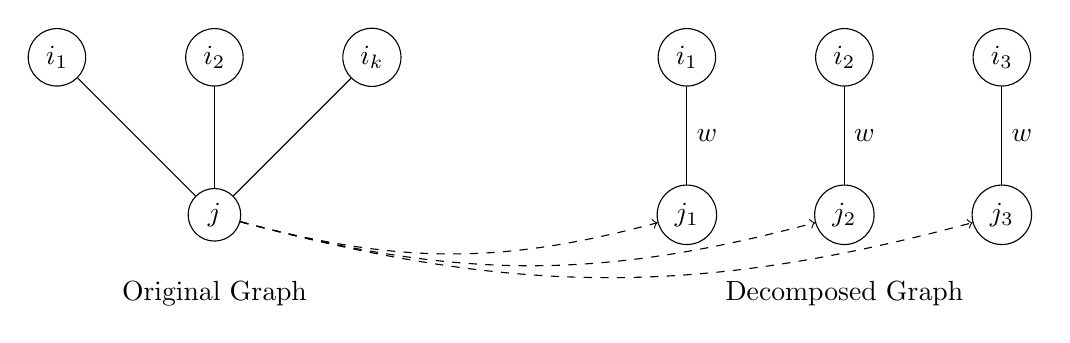
\begin{tikzpicture}
  % Original bipartite graph on the left
  \node[draw, circle] (j) at (-2,0) {$j$};
  \node[draw, circle] (i1) at (-4,2) {$i_1$};
  \node[draw, circle] (i2) at (-2,2) {$i_2$};
  \node[draw, circle] (i3) at (0,2) {$i_k$};
  
  \draw (i1) -- (j);
  \draw (i2) -- (j);
  \draw (i3) -- (j);
  
  \node at (-2,-1) {Original Graph};

  % Decomposed bipartite graph on the right
  \node[draw, circle] (j1) at (4,0) {$j_1$};
  \node[draw, circle] (j2) at (6,0) {$j_2$};
  \node[draw, circle] (j3) at (8,0) {$j_3$};
  
  \node[draw, circle] (di1) at (4,2) {$i_1$};
  \node[draw, circle] (di2) at (6,2) {$i_2$};
  \node[draw, circle] (di3) at (8,2) {$i_3$};

  \draw (di1) -- (j1) node[midway, right] {$w$};
  \draw (di2) -- (j2) node[midway, right] {$w$};
  \draw (di3) -- (j3) node[midway, right] {$w$};
  
  \node at (6,-1) {Decomposed Graph};

  % Connecting original and decomposed graphs
  \draw [dashed, ->] (j) to [out=345,in=195] (j1);
  \draw [dashed, ->] (j) to [out=345,in=195] (j2);
  \draw [dashed, ->] (j) to [out=345,in=195] (j3);
\end{tikzpicture}
\caption{Decomposition of a general graph to a star graph in the solution approach.}\label{fig:graph_decompose_AE}
\end{figure}

In this revision, we have underscored the principles underlying this decomposition via the following corollary. At one extreme, a weight of $w=1$ provides an aggressive approximation, in which the formulation allows each customer $j\in\calC$ to be covered $|\calF_j|$ times. Vice versa, a weight of $w=1/d_\star$ provides a conservative approximation in which each customer $j\in\calC$ can be covered at most once. This result motivates our algorithm, which searches over the weight of the decomposition.
\begin{corollary}\label{cor:heuristic}
Let $m^S(w)$ be the optimum of Problem $(\calP_N^\dagger)$ in the star graph $\calG_w$ with weights $\text{deg}(i)=w|\calC_i|$, and $m^\dagger$ the one of Problem $(\calP_N^\dagger)$. Then $m^S(1) \leq m^\dagger \leq m^S(1/d_\star)$.
\end{corollary}

Another possibility would be to add degrees of freedom via differentiated weights across facility-customer pairs, as shown in Figure~\ref{fig:graph_decompose_granular_AE}. Again, the weights would lead to upper and lower bounds, but the more granular decomposition would provide more degrees of freedom to derive higher-quality solutions. On the other hand, this would require searching over an exponentially larger space in $\calO(W^{|\calF||\calC|})$ rather than $\calO(W)$, where $W$ is the number of values that each weight can take. This could be alleviated, for instance, by designing a tailored branch-and-bound algorithm for this problem, but this would require new developments to derive appropriate branching and bounding rules and, most importantly, to implement the algorithm in large-scale instances. Moreover, it remains unclear whether such an involved algorithm would be computationally scalable, given the very large dimensional search space in $\calO(W^{|\calF||\calC|})$, where $|\calC|=m$ grows infinitely large.

\begin{figure}[h!]
\centering
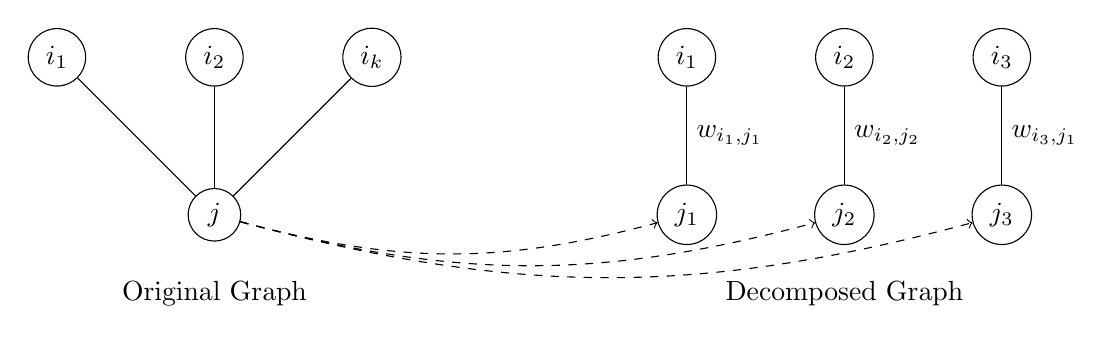
\begin{tikzpicture}
  % Original bipartite graph on the left
  \node[draw, circle] (j) at (-2,0) {$j$};
  \node[draw, circle] (i1) at (-4,2) {$i_1$};
  \node[draw, circle] (i2) at (-2,2) {$i_2$};
  \node[draw, circle] (i3) at (0,2) {$i_k$};
  
  \draw (i1) -- (j);
  \draw (i2) -- (j);
  \draw (i3) -- (j);
  
  \node at (-2,-1) {Original Graph};

  % Decomposed bipartite graph on the right
  \node[draw, circle] (j1) at (4,0) {$j_1$};
  \node[draw, circle] (j2) at (6,0) {$j_2$};
  \node[draw, circle] (j3) at (8,0) {$j_3$};
  
  \node[draw, circle] (di1) at (4,2) {$i_1$};
  \node[draw, circle] (di2) at (6,2) {$i_2$};
  \node[draw, circle] (di3) at (8,2) {$i_3$};

  \draw (di1) -- (j1) node[midway, right] {$w_{i_1,j_1}$};
  \draw (di2) -- (j2) node[midway, right] {$w_{i_2,j_2}$};
  \draw (di3) -- (j3) node[midway, right] {$w_{i_3,j_1}$};
  
  \node at (6,-1) {Decomposed Graph};

  % Connecting original and decomposed graphs
  \draw [dashed, ->] (j) to [out=345,in=195] (j1);
  \draw [dashed, ->] (j) to [out=345,in=195] (j2);
  \draw [dashed, ->] (j) to [out=345,in=195] (j3);
\end{tikzpicture}
\caption{Stronger decomposition of a general graph to a star graph.}\label{fig:graph_decompose_granular_AE}
\end{figure}

At this point, we believe that a more involved computational algorithm for $(\calP^\dagger_G)$ falls beyond the scope of the paper. It would take extensive new developments at the end of the last section to bring it to fruition, which would add more complexity to a paper that is already long and technical. Moreover, these developments would depart from the main techniques used in the paper, by focusing on computational algorithms rather than the theoretical analysis of the online learning and optimization algorithm. Finally, these developments would be tailored to Problem $(\calP^\dagger_G)$, with limited generalizability to broader optimization problems. We have mentioned the development of stronger algorithms for Problem $(\calP^\dagger_G)$ as an opportunity for future research in the conclusion.
\begin{quote}
    ``Another avenue lies in developing exact algorithms for the deterministic approximation model in the networked setting.''
\end{quote}

\begin{commentBox}
\textbf{Comment 7. Major comments: Numerical analysis.}\label{AE:7}

R3 asks for a more detailed numerical analysis that could perhaps apply the algorithms to one of the motivating examples (clinical trials, retail stores, etc...) I would not think about this as a requirement, but certainly a computational exercise on a (near) real world problem would do well to build more insight into the behavior of the algorithms and strengthen the contribution.
\end{commentBox}

We appreciate the flexibility that you have given us. We have actually conducted new computational experiments to demonstrate the practical applicability of our approach on real-world datasets. This extension addresses three important aspects of our methodology. First, it provides guidance on how the algorithm can be applied in real-world contexts---by fitting a machine learning model at each iteration rather than relying on reduced-form expressions of out-of-sample error rates. Second, it addresses the robustness of our method outside of the asymptotic regime, by demonstrating the performance improvements of the proposed online and optimization procedure over the no-learning baseline even when the coverage target is finite and limited. Third, it provides empirical evidence of the quality of the learning function by showing that it provides a good approximation of out-of-sample performance of data-driven machine learning models in our (non-i.i.d.) online learning and optimization process, thus complementing our newly-added theoretical results discussed in response \hyperref[AE:5]{\color{blue}Comment 5}. We provide further details on this revision below.

We apply our online learning and optimization framework to four datasets from the \cite{UCI} featuring binary classification with multivariate data, 10--100 attributes, more than 1,000 records, and structured data: ``bank marketing'', ``default of credit card clients'', ``occupancy detection'' and ``online shoppers purchasing intention''. Table~\ref{tab:dataset_AE} reports descriptive statistics on the datasets.

\begin{table}[h!]
\centering \small
\caption{Descriptive statistics of the 10 datasets and corresponding data-driven experimental setup.}
\label{tab:dataset_AE}
\renewcommand{\arraystretch}{1.3}
\begin{tabular}{lllllll}
\toprule[1pt]
Dataset & Positive class & \# observations & \# features & Positive rate & Best fit\\ \midrule[0.5pt]
Bank & 521 & 4,521 & 16 & 11.5\% & $\frac{1}{n^{0.584}}+0.12$ \\
Default & 6,636 & 30,000 & 23 & 22.1\% & $\frac{0.69}{n^{0.703}}+0.18$ \\
Occupancy & 2,049 & 9,752 & 6 & 21.0\% & $\frac{0.19}{n^{0.544}}+0.01$\\
Online & 1,908 & 12,330 & 6 & 15.5\% & $\frac{0.71}{n^{0.635}}+0.08$ \\
\bottomrule[1pt] 
\end{tabular}
\end{table}

The first objective is to show that the learning function considered in the mathematical formulation (Assumption~\ref{ass:classification_AE}) provides a good approximation of out-of-sample performance of real-world machine learning models, even with non-i.i.d. samples obtained through the online learning and optimization process defined in Section 3 of the paper. To this end, we replicate this process in these experiments. For every dataset, we train a random forest classification model, randomly select 10 samples with positive predictions from the current classification model to serve as training samples for the next round, and proceed iteratively. We repeat the procedure 10 times for each dataset. 

Figure~\ref{fig:ML_AE} reports the improvement in predictive performance as a function of the accrued sample size under this online learning environment, thereby providing empirical evidence for the learning function in Assumption~\ref{ass:classification_AE}. The figure plots the out-of-sample classification error as a function, averaged across the ten instances. At each iteration, the out-of-sample classification error is calculated using all samples that have not been utilized for training. Table~\ref{tab:dataset_AE} and Figure~\ref{fig:ML_AE} also report the best fits of the form $\frac{\gamma}{n^r}+\beta$ (which corresponds to Assumption~\ref{ass:classification_AE}). These results suggest a clear downward trend as the sample size increases, as well as a concave dependency indicating diminishing returns as the sample size becomes increasingly large. The fitted curves yield a good first-order approximation of the learning error, so that the assumption that the learning error decay in $\calO(1/n^r)$ characterizes fairly well the impact of additional data points on predictive performance---even in our online learning environment where data samples are not independent over time. Ultimately, these results complement our statistical learning results with an empirical justification of the general-purpose characterization of the machine learning model in our theoretical analysis.

\begin{figure}[h!]
	\centering
	\subfloat['Bank' dataset.]{\label{fig:bank_AE}\includegraphics[width=.49\textwidth]{figures/ML_bank.pdf}}
    \hspace{2pt} 
	\subfloat['Default' dataset.]{\label{fig:default_AE}\includegraphics[width=.49\textwidth]{figures/ML_default.pdf}}
    \hspace{2pt} 
	\subfloat['Occupancy' dataset.]{\label{fig:ccupancy_AE}\includegraphics[width=.49\textwidth]{figures/ML_occupancy.pdf}}
    \hspace{2pt} 
	\subfloat['Online' dataset.]{\label{fig:online_AE}\includegraphics[width=.49\textwidth]{figures/ML_online.pdf}}
	\caption{Average error of the classification models as a function of the accrued sample size. The red curve shows the best fit of the form $\frac{\gamma}{n^r}+\beta$.}
    \label{fig:ML_AE}
    \vspace{-12pt}
\end{figure}

Next, we estimate the performance of the proposed online learning and optimization approach. For each dataset, we treat each data point as a candidate ``facility'' and we impose a target of $m=n/10$ over $T=2$ time periods, where $n$ is the size of the dataset, so that the target is large enough and the candidate pool also remains large enough. At each iteration, we train a random forest model based on the past samples; we select items among the sub-population with positive predictions; and we observe success realizations based on the ground-truth labels. We compare the solution to a no-learning benchmark that selects samples uniformly at random until $m$ positive samples are obtained. For each dataset, we replicate each simulation 100 times.

Figure~\ref{fig:ML_real_AE} shows that the online learning and optimization procedure significantly outperforms the no-learning baseline, requiring far fewer samples to achieve the same coverage target---even over two iterations. Specifically, it reduces the cost by over 50\% across all datasets, and by an order of magnitude for the ``online'' dataset. Moreover, the benefits are consistent across simulations, showing the robustness of the solution. The results provide empirical evidence, using real-world data, of the performance of the online learning and optimization approach developed in the paper.

\begin{figure}[h!]
    \centering
    \includegraphics[width=.8\textwidth]{figures/ML_real.pdf}
    \caption{Number of samples required to identify $m=n/10$ positive samples across datasets ($\delta=5\%$).}
    \label{fig:ML_real_AE}
\end{figure}

In conclusion, this revision has provided new empirical evidence of the quality of the statistical learning function (motivated by our new theoretical results), and of the performance of the algorithm developed in this paper in real-world and finite-sample settings. Thank you for pushing us in that direction, which has clearly enhanced the practical contributions of the paper.

\begin{commentBox}
\textbf{Comment 8. Minor comments.}\label{AE:8}

\begin{enumerate}
    \item Page 8, learning environment paragraph, ``we encode''
    \item Page 10, benchmarks discussion. I did not follow the non-learning baseline, but this is related to the issues with the uncertainty model that have already been raised.
    \item It might be useful to expand on the caption of Table 1 to explain the diagonal entries.
    \item Page 24, definition of $\calF^{CTL}$. Should it be $\deg(i)$ instead of $\deg(j)$?
    \item Theorem 5, extra period after first sentence.
    \item Lemma 4, where is the $\calN$ notation introduced?
\end{enumerate}
\end{commentBox}

We have fixed these minor issues and gone through the entire paper to check for any lingering typo. Specifically, we have corrected the text in response to points 1, 4 and 5. We have relegated Lemma 4 (Lemma EC.9 of the revised manuscript) to the appendix, upon defining $\calN(\by)$ as the set of facilities that are tentatively opened. And we have clarified that the no-learning baseline minimizes the number of facility openings subject the chance constraint, given that number of successful facilities follows a binomial distribution based on the initial error $\varepsilon$. This is formulated as follows in the core setting; as you mentioned, this is much more natural in view of the new statistical environment described in response to \hyperref[AE:5]{\color{blue}Comment 5}.
$$\min\quad \left\{A:\P\left[\Bino\left(A, 1- \varepsilon \right)\geq m\right] \geq 1-\delta\right\}$$

\vspace{12 pt}

Thank you again for your constructive and supportive report. We took all the comments from the review team very seriously and endeavored a complete overhaul of the paper in response. In particular, we have fully addressed the major concern regarding the mathematical formulation of the online learning and optimization paper, by formalizing the statistical environment and establishing the convergence properties of the online classifier. We have revised all our theoretical results and proof techniques as a result. Finally, we have studied new extensions to compare the static algorithm to an adaptive algorithm, and included new computational results to show the performance of the algorithm's solution in practice. The manuscript has significantly improved as a result.

\newpage
\section*{Response to Reviewer 1's Comments}
\addcontentsline{toc}{section}{\protect\numberline{}Response to Reviewer 1's Comments}%

\begin{commentBox}
\textbf{Comment 1.}\label{R1:1}

    I am very excited about the research question of this work, which is both new and relevant. However, I have significant concerns about the practicality of Assumption 1 and the robustness of the proposed approach without this assumption. The authors should carefully reconsider this assumption and either justify that the problem on page 10 is a valid problem to investigate or completely reframe the problem in a setting where the decision-maker learns the distribution of $v$, rather than the realizations.
\end{commentBox}

We are glad that you are very excited by the novelty and relevance of our research question. Indeed, the problem is prevalent in practice and novel in the literature, by combining online learning and online decision-making in an environment where each action simultaneously advance a strategic coverage objective and generate informative data for future decisions. This problem leads to inter-temporal dependencies that augment the belief state with a physical state. Moreover, the paper defines and studies a new asymptotic regime with an infinitely large coverage target but a limited planning horizon, which prevents the use of traditional explore-then-commit algorithms. We further discuss this regime in response to \hyperref[R1:7]{\color{blue}Comment 7}.

We understand your concerns regarding our statistical learning setting. In the original manuscript, this assumption was indeed \textit{positing} that the generalization error rate decays to 0 with the square root of the sample size. This assumption was based on standard statistical learning results, but your comments made us realize that these results could not be directly applied to our setting because our samples are not independent and identically distributed---precisely due to the online learning and optimization environment. Moreover, your comment emphasized that the zero error relied on the extra assumption that the features can be used to infer the realization of each unknown variable, which can be unrealistic. We have completely revised the statistical learning environment. Specifically, we now \textit{prove} that, under certain statistical conditions, our learning process converges to the optimal Bayes classifier at a rate of at best $\calO(1/\sqrt{n})$; notably, the online classifier learns the distribution of the uncertain parameters rather than the realizations themselves. This result provides one instantiation—rather than a unique characterization—of statistical conditions with these convergence properties; we then abstract away from this particular setup to formulate a general statistical learning function characterized by an initial error $\varepsilon$, a learning rate of order $\calO(1/n^{r})$, and an irreducible-error share of $1-p$; and we rigorously characterize the number of successful facilities via a binomial distribution under this statistical setting. This newly-added section provides necessary theoretical grounding to bridge our problem statement and the mathematical formulation, thereby enhancing the quality and rigor of the manuscript. For details, see our response to \hyperref[R1:6]{\color{blue}Comment 6} and to the newly-added Section 3.

We have therefore followed the two directions that you outlined in this summary: (i) we have developed a new statistical learning paradigm to justify our assumption and the resulting formulation of the online learning and optimization problem; and (ii) we reframed the problem in a setting where the decision-maker learns the distribution of the uncertain parameters rather than the realizations. We have also updated all results and all proofs; in particular, some changes required extensions of our main results and new proof techniques to account for the residual Bayes error and generalized learning rates in the online learning and optimization process. In addition to these issues, which you noted as ``by far [your] main concern with the [original] manuscript'' in \hyperref[R1:10]{\color{blue}Comment 10}, we have addressed all your other comments, as detailed in the remainder of this document.

In turn, the paper provides a true end-to-end approach to a new class of online and optimization problems. We begin by formalizing the online learning environment and proving that the error rate admits a precise upper bound with a specific functional form. Building on this foundation, we formulate a rigorous mathematical model, derive tight asymptotic lower and upper bounds up to the second-leading order, and develop a tractable and interpretable algorithm that yields an asymptotically-feasible and asymptotically-optimal solution. We show that the main insights are robust to different learning rates, different levels of irreducible error, offline data, and adaptive solution strategies. We then extend the full framework to a graph-based setting; despite a much more complex structure, we prove analogous results and develop a new deterministic algorithm with similar asymptotic guarantees. Finally, we validate the approach on synthetic data and on real-world data from the \cite{UCI}, providing evidence of both the quality of our statistical learning approximation and of the the practical benefits of our online learning and optimization algorithm. Together, these results offer a complete theoretical, algorithmic, and empirical foundation for a new class of online learning and optimization problems.

As a result, the revised manuscript is much stronger, more rigorous and more comprehensive. We appreciate your guidance in that regard and hope that this revision will address your concerns.

\begin{commentBox}
\textbf{Comment 2.}\label{R1:2}

    I believe that a paper potentially relevant to this work, which might help the authors in this endeavor, is \citep{che2023adaptive}. This work considers a small $T$ setting and transitions from an unknown distribution regime to a “known” distribution regime with Gaussians, where the variance is a function of past actions, and provides justification for this approximation.
\end{commentBox}

Thank you for the pointer. \cite{che2023adaptive} consider an adaptive experimentation problem with flexible batches and costly re-allocation of sampling effort. This is cast as a multi-armed bandit problem in a finite-horizon regime with asymptotically large batches in each period. The authors first define a statistical setting in which the average reward for each arm scales in $1/\sqrt n$, where $n$ is the batch size, and prove the validity of a Gaussian approximation for the sequential experiment. The statistical environment relies on distributional assumptions on the average reward for each arm, rather than individual rewards. The authors then cast the sequential experimentation problem as a Markov decision process, by updating the mean and standard deviation of the reward distribution for each arm, and develop dynamic programming algorithms to solve it.

You are correct that the asymptotic regime mirrors our limited planning horizon with an asymptotically large coverage target. This paper also uses similar concentration arguments and technical tools as in our paper (e.g., Lemma 2). Our paper also exhibits several differences. First, the discrete and irreversible decisions in our problem augment traditional multi-armed bandits structures with a physical state variable. In our core setting, we can view each arm as representing the set of facilities that have the same probability of success $\eta_{i}$. However, all successful facilities remain opened and contribute to overall coverage; this structure creates inter-temporal dependencies that augment the belief state with a physical state, and that complicate the design of exploration-exploitation dynamic programming algorithms. Second, \cite{che2023adaptive} assume that each arm's average reward follows a Gaussian and scales in $\calO(1/\sqrt n)$. In contrast, we make no apriori assumptions on the distributions of our ``rewards" $\eta_i$. In this revision, we show that, under statistical conditions, the online classifier converges to the optimal Bayes classifier at a rate of at best $\calO(1/\sqrt{n})$ (see our response to \hyperref[R1:6]{\color{blue}Comment 6}). Accordingly, we define a new learning environment with a generalized learning rate $\calO(1/n^r)$ and a residual error $1-p$. Third, we leverage proof techniques based on concentration inequalities rather than Gaussian approximations---namely, Hoeffding's inequality, Bernstein's inequality and the Berry-Esseen theorem.

We have added this reference to the literature review. This discussion underscores the similarities between the asymptotic regimes considered in the two papers. It also highlights that our paper defines a new class of problems in online learning and decision-making with discrete and irreversible decisions contributing to a target coverage, that it considers a different learning environment based on our new statistical results, and that it derives new technical results to obtain tight upper and lower bounds in that setting along with a constructive algorithm with guarantees of asymptotic feasibility and optimality. Thank you for helping us strengthen the positioning of the paper.

\begin{commentBox}
\textbf{Comment 3. Research question and contribution.}\label{R1:3}

    This paper considers the problem faced by a decision-maker who needs to cover demand by sequentially opening new facilities. Motivated by applications such as the opening of clinical trial sites, the authors assume that at each stage, the facilities that are tentatively opened may fail with a certain probability (unknown to the decision-maker). The goal is to minimize the number of attempted openings over the time horizon while satisfying a chance constraint that requires the target cover to be met with a sufficiently high probability. The trade-off emerging from this problem is that the decision-maker needs to open facilities to improve forecasts about the success of future facilities, but opening too many facilities increases the incurred cost.

    The paper designs and evaluates algorithms that achieve asymptotically first-order optimality (in a certain asymptotic regime where the coverage target and the chance constraint probability are scaled appropriately). The results are derived in a setting where customers and facilities are nodes in a bipartite graph, with each edge indicating that a customer could be covered by a facility if that facility is open. The paper establishes the asymptotic optimality of their algorithm under two conditions: i) each node has degree 1, or ii) a large number of facilities need to be open to meet the cover target.
\end{commentBox}

Thank you for summarizing the main characteristics of our problem---a novel online learning and optimization setting with irreversible decisions that contribute to a coverage target---and its technical contributions---deriving tight upper and lower bounds with a constructive algorithm in an asymptotic regime featuring an infinitely large coverage target but a limited planning horizon. As you mentioned, the result is proved both in a setting with homogeneous facilities and a supply-side target on successful facilities, and in a setting with heterogeneous facilities and a demand-side target on covered customers in a bipartite facility-customer graph. The results are similar in both cases, although the proof techniques are significantly more complex in the networked case (although, in this revision, we have considerably strengthened the results and proofs in the core setting).

As detailed below, we have strengthened these contributions in this revision. The major improvements, in response to your comments, lie in deriving statistical learning results to provide a more rigorous motivation of the problem, revising its formulation accordingly, and adapting the results and extending the proof techniques as a result. We have also addressed your other comments.

\begin{commentBox}
\textbf{Comment 4. Research question and contribution.}\label{R1:4}

    The research question is practically relevant, and the problem formulation is quite elegant. In particular, the authors’ emphasis on a small number of sequential decisions (small $T$) deviates from the classical perspective adopted in online learning.
\end{commentBox}

We are glad to learn that you enjoyed the relevance of the problem, the elegance of its mathematical formulation, and the novel asymptotic regime. Your comments are encouraging.

\begin{commentBox}
\textbf{Comment 5. Method.}\label{R1:5}

    While the research question is well-motivated, I have major concerns about some aspects of the execution.
\end{commentBox}

We also appreciate your concerns regarding the methodology. We address them in response to your comments below. In particular, we describe our new statistical learning results as well as their impact on the mathematical formulation, our main results, and some of the proof techniques. We understand from your report that this is your most important concern with our original manuscript; for your convenience, we provide in our response a detailed description of how we have addressed it in this revision, with pointers to the corresponding changes in the paper.

\begin{commentBox}
\textbf{Comment 6. Method.}\label{R1:6}

    I am quite puzzled by Assumption 1. First, it is not clear what the probability is taken with respect to. More importantly, the assumption suggests that as the number of samples increases, the ML model will almost exactly determine whether each facility will succeed or not. Usual error bounds are compared to Bayes-optimal classifiers (see papers cited on page 9). Here, the extra assumption is that the Bayes-optimal classifier would provide perfect predictions (i.e., features can be used to perfectly infer the value of $v$). In my view, this is a very strong assumption and not very practical. I am concerned that this assumption is critical to the results developed, as the authors ultimately analyze the problem described on page 10, in which the success probability of selected facilities converges to 1. A more realistic assumption would be that the decision-maker learns the distribution (as opposed to the realizations) of $v$—i.e., facilities have different success probabilities, and as the number of samples grows, the ML model learns the success probability. Furthermore, most of the papers cited on page 10 to justify this assumption deal with offline learning, which does not account for the potential bias in forecasts arising when making adaptive decisions (which is the focus of this work).
\end{commentBox}

This comment refers to our main assumption in the original manuscript that the generalization error decays to 0 with the square root of the sample size. For your convenience, we replicate it below; note that, in this revision, we have changed the notation of the ``true'' success realization from $v_{it}$ to $S_{it}$ and we adopt this new notation here for consistency.
\setcounter{assumption}{0}
\begin{assumption}[Original manuscript] \label{ass:classification_old_R1}
    There exists $0<\varepsilon\leq 1$ such that the error of the machine learning model $f_t$ trained with $N_{t-1}$ samples is bounded by:
    \begin{align*}
         \P_{t}(f_t(\bx_{it})\neq S_{it})\leq \frac{\varepsilon }{\sqrt{N_{t-1} + 1}}.
    \end{align*}
    
\end{assumption}

In the original manuscript, we had justified this assumption from statistical learning theory \citep[using, for instance][]{chaudhuri2014rates,ng2001discriminative,mansour2000generalization,ng2001discriminative,gao2020towards}. However, your comment made us realize that this assumption was problematic. Indeed, we had not rigorously specified the probability space of the learning process. In fact, the samples are not independent in our online environment due to intertwined learning and optimization---namely, the decisions focus on the subset of facilities with a positive prediction. This prevents the direct application of the statistical learning results that we cited, which often rely on i.i.d. samples. Second, we implicitly assumed that the machine learning model can learn the success/failure realizations, as opposed to learning the distribution. As you noted, this also prevents the direct application of statistical learning results, which usually derive error bounds from Bayes-optimal classifiers.

We have overhauled this assumption in this revision. We now formalize our statistical learning setting in an environment where the true success/failure realizations are not perfectly determined by the features---that is, where the Bayes-optimal classifier may not yield perfect predictions. We now prove that, under some statistical conditions, the classifier in our online learning and optimization process converges to the Bayes-optimal classifier at a rate of at best $\calO(1/\sqrt{n})$. We outline the main result in the informal proposition below, and provide details thereafter (Proposition~\ref{prop:MLE_R1}).
\setcounter{proposition}{0}
\begin{proposition}[Revised manuscript, informal]\label{prop:MLE_informal_R1}
       Under statistical learning conditions, the error rate of the learned classifier, denoted by $\mu_t$ converges to that of the Bayes-optimal classifier, denoted by $\mu^*$, as follows, for some $\alpha>0$, for any $\varepsilon,\gamma>0$, and for $N_{t-1}$ large enough:
        \[\mu_t \leq \frac{\overline\varepsilon}{(N_{t-1}+1)^{\min\{\alpha,1\}\times (1/2-\gamma)}}+\mu^*.\]
\end{proposition}

We emphasize that this construction serves as one instantiation—rather than a unique characterization—of statistical conditions under which these convergence properties would hold. Importantly, these statistical conditions solely support the convergence assumption of the classifier and are not invoked in the derivation of our regret bounds and other results in the online learning and optimization problem.

Let us now provide details on these new developments, which address your comments by closely following the newly-added Section 3 of the paper.

\paragraph{Online dynamics.}
Let $\calF$ denote the set of $M$ candidate facilities. A decision-maker targets to open $m$ facilities over $T\geq 2$ periods, stored in a set $\calT=\{1,\cdots,T\}$. We encode these decisions via the following variables:
\begin{align*}
    y_{it}&=\begin{cases}
        1&\text{if the decision-maker attempts to open facility $i\in\calF$ at time $t\in\calT$}\\
        0&\text{otherwise.}
    \end{cases}
\end{align*}

Let $S_{it}$ denote the binary indicator of the success of facility $i\in\calF$ at time $t\in\calT$. We assume that success is revealed by the next period and is independent across facilities. We define the following variables:
\begin{equation}\label{eq:z_R1}
    z_{it} = \begin{cases}
        1 & \text{if facility $i\in\calF$ is open at time $t\in\calT$, i.e. if}\ S_{it} = 1 \;\; \text{and}\;\; y_{it}=1\\ 
        0 & \text{otherwise, i.e., if}\ \text{if}\ S_{it} = 0 \;\; \text{or}\;\; y_{it}=0
    \end{cases}
\end{equation}
Let $A_t=\sum_{i\in\calF}y_{it}$ and $B_t=\sum_{i\in\calF}z_{it}$ be the number of facilities tentatively and successfully opened at time $t\in\calT$. The decision-maker aims to minimize $\sum_{t=1}^T A_t$ subject to a chance constraint ensuring that $m$ facilities will be opened with high probability: $\P\left[\sum_{t=1}^TB_t\geq m\right]\geq1-\delta$. To formulate this problem, we need to relate the decisions $A_t$ to the random variables $B_t$.

Throughout the paper, we consider the asymptotic regime where $m\to\infty$ but where $T\geq2$ is finite. Assumption~\ref{ass:regime_R1} defines an asymptotic regime with a large-enough pool of candidate facilities, to enable sampling among unexplored facilities.
\setcounter{assumption}{0}
\begin{assumption}[Asymptotic regime]
    \label{ass:regime_R1}
   As $m \to \infty$, $M=\Omega(m^{3/2})$.
\end{assumption}

\paragraph{The learning environment.}
The original manuscript implicitly assumed that the machine learning model could learn the success/failure \textit{realizations}, as opposed to learning the \textit{distribution}. In the revised manuscript, we instead consider an environment where the distribution of facility success can be learned; that is, the machine learning model no longer learns the success realizations but the success probabilities.

We denote by $\eta_{i} \in [0,1]$ the (unknown) probability of success of facility $i\in\calF$, so that facility success is governed by a Bernoulli random variable $S_{it}\sim \text{Ber}(\eta_{i})$. Each facility $i\in\calF$ is associated with a feature vector $\bx_{i} \in \calX\subseteq\R^{p_t}$.

The learning population consists of the set of facilities that have been tentatively opened, so the decision-maker has access to the following data sample at each period $t\in\calT$, of size $N_{t-1}=\sum_{s=1}^{t-1}A_s$.
$$\calS_t=\left\{(\bx_{i},z_{is})\mid s\in\{1,\cdots,t-1\}\ ;\ i\in\calF:y_{is}=1\right\}$$

The decision-maker can then train a classification model to predict the binary indicators $S_{it}$ for the remaining $M-N_{t-1}$ facilities. Let $\calD^n = \calX^n\times\{0,1\}^n$ denote the space of datasets of size $n$, and $\calD = \bigcup_{n=1}^\infty \calD^n$ the space of all finite datasets. We define the set of hypotheses $\calH = \{h: \calX \to \{0,1\} \mid \Phi(h) \leq 0\}$, where $\Phi(\cdot)$ limits available models. A classification algorithm $F: \calD \to \mathcal{H}$ is a function mapping from $ \calD$ to $\calH$. The classification model in period $t\in\calT$ is denoted by $h_t = F(\mathcal{S}_t)$.

To define the sampling process, we assume that there exists a non-negligible fraction of positive samples in the population. Combined with Assumption~\ref{ass:regime_R1}, this implies that the pool of positive instances remains large enough over time. Otherwise, it would become impossible to select $A_t$ positive instances, and the overall online learning and optimization problem would be infeasible. Note that the cutoff of $1/2$ arises from symmetric misclassification penalties, but our framework can be easily generalizable otherwise through reweighting of the loss function.
\begin{assumption}[Existence of Positive Samples]\label{ass:positive_R1} There exists a constant $\xi > 0$ such that at least a fraction $\xi$ of the sample has a success probability greater than $1/2$.
\end{assumption}

We then assume that the decision-maker treats facilities interchangeably in the sampling process.

\begin{assumption}[Sampling]\label{ass:sampling_R1}
    At each time period $t\in\calT$, the decision-maker selects facilities randomly with replacement among the set of unexplored facilities with a positive classification, denoted by $\calJ_t=\{i\in\calF\mid y_{i1}=\cdots=y_{i,t-1}=0\ ;\ h_t(\bx_{i})=1\}$. Thus, $\P\left(y_{it}=1 \mid i \in \calJ_t\right)= 
    \frac{A_t}{|\calJ_t|}$.
\end{assumption}

One limitation in Assumption~\ref{ass:sampling_R1} is that it allows for the same facility to be selected multiple times in the same period. Yet, under Assumptions~\ref{ass:regime_R1} and~\ref{ass:positive_R1}, the size of the eligible pool $|\calJ_t|$ asymptotically dominates the number of selections $A_t$. Thus, the probability of selecting the same facility multiple times is asymptotically small. Alternatively, we could assume that facilities are sampled without replacement, which would induce negative correlation among the $y_{it}$ variables. In that case, standard results from concentration theory \citep{serfling1974probability} would lead to slightly tighter concentration bounds and all results from the paper would hold. Our modeling choice serves as a standard simplification that facilitates the analysis without materially affecting the results. Such simplifications are common in statistical frameworks—e.g., in Neyman's repeated sampling paradigm from an asymptotically large superpopulation \citep{Neyman1934,SarndalSwenssonWretman1992}.

Finally, we make the following non-parametric assumption on the learning rate, described by an initial error $\varepsilon$, a learning rate of order $\calO(1/n^{r})$ with $r>0$, and an irreducible-error share of $1-p$:
\begin{assumption}[Learning function] \label{ass:classification_R1}
    There exists $0<\varepsilon\leq 1$ such that the error of the machine learning model $h_t$ trained with $\calS_t$ ($N_{t-1}$ samples) is bounded by:
    \begin{align*}
        \P(h_t(\bx_{i})\neq S_{it} \mid i \in \calJ_t)=\frac{\varepsilon\cdot p}{\left(N_{t-1} + 1\right)^r}+\varepsilon\cdot(1-p).
    \end{align*}
\end{assumption}

This is the core assumption on the learning function. Note that we have generalized it from the original submission, by allowing a residual error $1-p$ (encapsulating the Bayes error rate, as you suggested) and a generalized learning rate. Whereas the functional form of the error bound resembles classical results in statistical learning theory \citep{boucheron2005theory, vapnik2015uniform, bousquet2002stability, feldman2019high}, the key distinction lies in the dependence structure of the data. Both the observed dataset $\calS_t$ and the candidate pool $\calJ_t$ are adaptively generated and inherently biased toward instances with positive predictions. Specifically, the set of facilities that can be selected at period $t$ depends on the classification model at period $t$, which itself depends on the set of facilities that are opened in periods $1,\cdots,t-1$. This feedback loop violates standard i.i.d. assumptions, so standard generalization bounds cannot be directly applied. In response, we introduce a statistical learning environment that explicitly models the dependence structure and demonstrates that bounds of the same functional form can still be achieved. As mentioned above, the statistical environment serves as one instantiation—rather than a unique characterization—of statistical conditions under which these convergence properties would hold, but similar convergence results could be obtained in different statistical setups. In the remainder of the paper, we therefore abstract away from the particular statistical conditions to formulate a more general statistical learning function.

\paragraph{A statistical learning setup.}

We define a generative model of the success probabilities as a function of the features $\bx_{i}$. We do not make distributional assumption on the functional form of $f_\theta$. The classification model involves estimating the parameter $\theta\in\Theta$.
\setcounter{stat}{0}
\begin{stat}[Generative model]\label{ass:known_R1}
The success probabilities are determined by the features: $\eta_{i} = f_\theta(\bx_{i})$, where $f_\theta:\calX\to[0,1]$ is known and $\theta\in\Theta$ is a finite set of parameters. 
\end{stat}

We make a margin assumption that $f_\theta$ features a limited concentration around $0.5$, which is commonly used in statistical learning theory \citep[e.g.,][]{boucheron2005theory, tsybakov2004optimal}.
\begin{stat}[Margin]\label{ass:margin_R1}
$\P\left(\left|f_\theta(\bx_{i})-\frac{1}{2}\right|\leq\nu\right)\leq C \nu^{\alpha}$ for some $C>0$ and $\alpha>0$.
\end{stat}

We also impose the following regularity condition on the generative function $f_\theta$.
\begin{stat}[Regularity]\label{ass:regularity_R1}
\begin{enumerate}
    \item $\Theta$ is a compact set and $\mathcal{X}$ is a compact set.
    \item $f_\theta(\bx)$ is a twice continuously-differentiable function of $\theta$ uniformly in $\bx \in \mathcal{X}$, and $f_\theta(\bx)$ is a continuous function in $\bx$ for every $\theta$. 
    \item The conditional Fisher information matrix is positive definite for all $\bx\in\calX$:
    \[\mathcal{I}(\bx,\theta) = \frac{1}{f_\theta(\bx)(1-f_\theta(\bx))}\frac{\partial f_\theta(\bx)}{\partial \theta}\frac{\partial f_\theta(\bx)}{\partial \theta^T} \]
\end{enumerate}
\end{stat}

Next, features are not influenced by decisions, which is also common in online learning.

\begin{stat}[Features]\label{ass:features_R1}
    Features are sampled from distribution $\calQ$:
    $\bx_{i}\sim \calQ$.
\end{stat}

We can then define the Bayes-optimal classifier $h^*(\bx)=\mathbf{1}\left\{f_\theta(\bx)>\frac{1}{2}\right\}$ and its error rate $\mu^*$ as follows.  The threshold of $1/2$ arises from symmetric misclassification penalties, but can be easily generalized to any misclassification penalties and any classification threshold.
$$\mu^*=\P(z_{it}\neq1 \mid h^*(\bx_i)=1)=1-\frac{\sum_{i\in\calF:\eta_{i}>\frac{1}{2}}f_\theta(\bx_{i})}{\left|i\in\calF:f_\theta(\bx_{i})>\frac{1}{2}\right|}$$

\subsubsection*{Rate of convergence.}
We can now prove that the online classifier converges to the Bayes-optimal classifier at a rate $\calO(n^{-\min\{\alpha,1\}\times (1/2-\gamma)})$ for any $\gamma>0$, where $n$ is the sample size accrued over time. As expected, convergence is faster with larger values of $\alpha$, which reflects an easier online learning setting if the generative function has a wider margin from 0.5. Moreover, the best possible convergence rate under these assumptions is $\calO(\sqrt n)$.
\setcounter{proposition}{0}
\begin{proposition}\label{prop:MLE_R1}
       Assume that we estimate $\theta$ using the maximum likelihood estimator (MLE):
    \begin{equation}
        \widehat{\theta}_t= \argmax_{\theta\in\Theta} \ \prod_{s=1}^{t-1} \prod_{i\in\calJ_s:y_{is}=1} (f_\theta(\bx_{i}))^{z_{is}}(1-f_\theta(\bx_{i}))^{1-z_{is}}, \label{eq:mle_estimation_R1}
    \end{equation}
    and build the classifier
    $h_t(\bx_{i}) = \mathbf{1}\left\{f_{\widehat{\theta}_t}(x_{i})>\frac{1}{2}\right\}$. Define the error rate $\mu_t = \P(S_{it}\neq 1 \mid i\in\calJ_t)$. Assume that $N_t \to \infty$ as $m \to \infty$ for all $t$. Under Assumptions~\ref{ass:regime_R1}-\ref{ass:positive_R1} and Statistical Conditions~\ref{ass:known_R1}--\ref{ass:features_R1}, for any $\overline\varepsilon,\gamma>0$, there exists $m_0$ such that for all $m\geq m_0$ and $t\in\calT$:
    \[\mu_t \leq \frac{\overline\varepsilon}{(N_{t-1}+1)^{\min\{\alpha,1\}\times (1/2-\gamma)}}+\mu^*.\]
\end{proposition}

The proof (in EC.1) bounds the difference between the classifier's error rate and the Bayes-optimal error by: (i) the sampling probability of each facility across earlier time periods; (ii) the probability that the true success probability lies around 0.5; and (iii) the classifier's error. We show that these terms are respectively bounded by $\calO(1/N_{t-1}^{1/2-\gamma})$, $\calO(1/N_{t-1}^{\alpha\cdot(1/2-\gamma)})$, or $\calO(1/N_{t-1}^{1/2})$.

\paragraph{Implications on the problem formulation.}

Importantly, the upper bound in Proposition \ref{prop:MLE_R1} matches Assumption \ref{ass:classification_R1} with $\varepsilon = \overline\varepsilon + \mu^*$ and $p=\frac{\overline\varepsilon}{\overline\varepsilon+\mu^*}$; the learning rate $\calO(1/n^r)$ generalizes the best-case rate of $\calO(\sqrt n)$ identified in Proposition~\ref{prop:MLE_R1}. In particular, if $\alpha<1$ characterizes a weak margin separation, the online classifier converges at a slower rate $r<0.5$ per Proposition \ref{prop:MLE_R1}. More generally, Assumption \ref{ass:classification_R1} covers a wider range of noise structures, data-generating processes, and model-misspecifications than Statistical Conditions~\ref{ass:known_R1}–\ref{ass:features_R1}.

We further note that Assumption \ref{ass:classification_R1} also brings a key simplification. Under Proposition \ref{prop:MLE_R1}, the error $\mu_t$ in period $t$ is only bounded above by a term that depends on the number of past trials; in principle, $\mu_t$ may still vary with the realized data $(\bx_s,z_{is})$. Assumption \ref{ass:classification_R1} adopts that upper bound itself as the error rate, which depends solely on the count $N_{t-1}$ and does not depend on the particular outcomes. This feature lets us cleanly couple the learning and optimization parts of the model without tracking the full history.

The next result confirms that this simplification is conservative for our chance-constraint:
\setcounter{corollary}{0}
\begin{corollary}[Learning environment] \label{cor:learning_R1}
    Define independent Bernoulli variables\\$\widetilde{S}_{it}=\Bern\left(1-\frac{\varepsilon\cdot p}{\left(N_{t-1} + 1\right)^r}-\varepsilon\cdot(1-p)\right)$ and $\widetilde{B}_t = \sum_{i:y_{it}=1} \widetilde{S}_{it}$, with $r=\min\{\alpha,1\} \times \{1/2-\gamma\}$, $\varepsilon = \overline\varepsilon + \mu^*$, and $p = \frac{\overline\varepsilon}{\overline\varepsilon+\mu^*}$. Then, $\P\left[\sum_{t=1}^T\widetilde{B}_t\geq m\right] \leq \P\left[\sum_{t=1}^TB_t\geq m\right]$.
\end{corollary}
Consequently, any policy we design under Assumption \ref{ass:classification_R1} already respects the chance constraint under Proposition~\ref{prop:MLE_R1}. Corollary \ref{cor:learning_R1} therefore provides the essential link, so the rest of the analysis can proceed with only Assumptions \ref{ass:regime_R1}--\ref{ass:classification_R1}, rather than the full set of statistical conditions~\ref{ass:known_R1}–\ref{ass:features_R1}.

We can then characterize the distribution of the number of successful facilities $B_t$ at each time period $t\in\calT$.
\begin{corollary}[Success Distribution]\label{cor:success_R1}
    Under Assumptions~\ref{ass:regime_R1},~\ref{ass:sampling_R1} and \ref{ass:classification_R1}, $B_t$ follows a binomial distribution with $A_t$ trials and success probability $1- \frac{\varepsilon\cdot p}{\left(N_{t-1} + 1\right)^r}-\varepsilon\cdot(1-p)$. 
\end{corollary}

These two corollaries complete the bridge from our problem statement to its mathematical formulation, enabling us to formulate our problem $(\calP^*)$ as follows:
\begin{align}
    \min\quad & \sum_{t=1}^T A_t \label{prob:main_R1}\tag{$\calP^*$}\\
    \st\quad&\P\left[\sum_{t=1}^TB_t\geq m\right] \geq 1-\delta \nonumber\\
    \quad& B_t\sim \Bino\left(A_t, 1- \frac{\varepsilon\cdot p}{\left(\sum_{s=1}^{t-1} A_s +1\right)^r}-\varepsilon\cdot(1-p)\right),\ \forall t\in\calT\nonumber\\
    \quad& A_t,B_t\geq0,\ \forall t\in\calT\nonumber
\end{align}

\paragraph{Implications on our online learning and optimization results.}\

We have revised our results and proofs to reflect the setting given by Assumption~\ref{ass:classification_R1}. In particular, we have extended all our results to accommodate different learning rates and Bayes error rates. Accordingly, we measure regret against a fully-learned benchmark with the asymptotic error $\varepsilon (1-p)$, that is, against a benchmark that has access to the Bayes-optimal classifier in advance. This benchmark needs to open at least $\frac{m}{1-\varepsilon\cdot(1-p)}$ facilities to satisfy the chance constraint.

\textit{New result.}
Theorem~\ref{thm:main_R1} identifies an asymptotically-tight sub-linear regret bound, and shows that the solution from Algorithm 1 of the paper is asymptotically feasible and asymptotically optimal up to the second-leading order. Thus, the theorem provides tight upper and lower bounds, as well as a constructive algorithm that achieves them. When $p=1$ or $\alpha_T(1-r)\geq1/2$, we obtain matching bounds up to the second leading-order rate and coefficients; otherwise, we obtain matching bounds up to the second leading-order rate. Our main result in the original paper considered the case with $r=0.5$ and $p=1$; this new theorem extends the result to any value of $r>0$ and $p\in[0,1]$. This theorem makes use of the following definitions:
\begin{align*}
	\alpha_T=\frac{1}{1-r^T}\qquad\qquad
	\zeta_T=\frac{\frac{1}{r^T}-1}{1-r}\cdot\left(\frac{1}{r}\right)^{\frac{r}{1-r}-T\alpha_T}\cdot c_0^{\alpha_T\cdot(1-r)} \qquad\qquad c_0 = \frac{1}{1-(1-p)\varepsilon}
\end{align*}
\setcounter{theorem}{0}
\begin{theorem}\label{thm:main_R1}
	The optimal solution $m^*(\varepsilon, T)$ of Problem $(\calP^*)$ satisfies, as $m \to \infty$:
    $$m^*(\varepsilon, T)\geq \begin{cases}
      c_0\left(m +\max\left\{-\Phi^{-1}(\delta)\sqrt{2\varepsilon(1-p)m}, \varepsilon \cdot p \cdot \zeta_T\cdot m^{\alpha_T\cdot(1-r)}\right\}+o\left(m^{\alpha_T(1-r)}\right)\right) & \text{if }p \neq 1,\\
          c_0\left(m +\varepsilon\cdot p\cdot\zeta_T\cdot m^{\alpha_T\cdot(1-r)} +  o\left(m^{\alpha_T\cdot(1-r)}\right)\right) & \text{if }p=1.
      \end{cases}$$
	Algorithm~\ref{ALG} yields an asymptotically feasible solution to Problem~\eqref{prob:main}, achieving an objective of:
    $$m^\dagger(\varepsilon,T)=\begin{cases}
        c_0\left( m+\varepsilon\cdot p\cdot \zeta_T \cdot m^{\alpha_T\cdot(1-r)} +  \sqrt{\frac{c_0}{2}\log \frac{2}{\delta}}\sqrt{m}\right) &  \text{if }p\neq 1,\\
   c_0\left( m+\varepsilon\cdot p\cdot \zeta_T \cdot m^{\alpha_T\cdot(1-r)} +  o\left(m^{\alpha_T\cdot(1-r)}\right)\right) &  \text{if }p=1.
    \end{cases}$$
\end{theorem}

\textit{New proof techniques.}
Our original proof could handle to some broader cases in the new theorem---modulo some new algebra---but other cases required new techniques. In the proof of Lemma 2 (to prove the asymptotic feasibility of the solution of Algorithm 1), Hoeffding's inequality may no longer lead to asymptotically tight bounds when $p=1$, so we leverage the Berry-Esseen theorem instead. This bounds the probability that at least $m$ facilities get successfully opened by the end of the planning horizon. In the proof of Lemma 3 (which establishes the lower bound), we use Bernstein's concentration inequality when $p=1$ to derive an asymptotically better bound than with Hoeffding's inequality, exploiting the fact that asymptotically, the error of the facility openings are small. When $p\neq1$, it uses the Berry-Esseen theorem to show that the lower bound is necessary to satisfy the chance constraint. We have carried these changes over to the networked case; in particular, we have replaced the concentration inequality from \cite{janson2004large} in dependency graphs by the recent result from \cite{janisch2024berry}, which extends the Berry-Esseen theorem in dependency graphs, to bound the difference between the number of customers covered by a successful facility and its expected value. These changes have elevated the technical depth of the results and proofs.

\paragraph{Robustness to the learning function.}

Theorem~\ref{thm:main_R1} demonstrates the robustness of our findings across a wide range of online learning regimes; in other words, our main result in the original manuscript was not driven by the idiosyncracies of the case with $p=1$ and $r=0.5$, but holds in a much broader set of learning regimes. Moreover, the theorem yields richer insights into the drivers of the regret bounds. As discussed in the original manuscript, larger values of $\varepsilon$ (i.e., higher uncertainty) lead to a higher regret from the perfect-information benchmark. The new result shows that the regret decreases as the learning rate $r$ increases and as the irreducible error $1-p$ decreases. They also identify additional insights on the interplay between the learning rate and the irreducible error. With perfect learning ($p=1$), the long-term regret rate converges to $\Theta\left(m^{1-r}\right)$; with imperfect learning ($p<1$), it converges to $\Theta\left(m^{1-r}\right)$ if $r\geq0.5$ but to $\Theta(\sqrt m)$ otherwise. In other words, if $p=1$ (perfect learning) or $\alpha_T(1-r)\geq1/2$ (slow learning, $r\lesssim0.5$), the main driver of regret lies in the learning rate; when $p<1$ (imperfect learning) and $\alpha_T(1-r)<1/2$ (fast learning, $r\gtrsim0.5$), the main bottleneck lies in the residual error due to imperfect learning.

\paragraph{Conclusion.}
This revised setting addresses your two comments. First, it specifies the probability space: at period $t\in\calT$, all facilities that have been selected are known to be successful or failed, meaning that the decision-maker has access to the true realizations $S_{i\tau}$ for $\tau=1,\cdots,t-1$. In turn, the relevant sample is restricted to the remaining facilities that have not been tentatively opened in previous time periods, by conditioning on $i\in\calJ_t$ in Proposition~\ref{prop:MLE_R1} and in Assumption~\ref{ass:classification_R1}. Then, the probability is taken over the data generating process and all the data used in the machine learning model, that is, over all possible datasets in $\calD^{N_{t-1}}$.

Second, the revision has relaxed the implicit assumption that the machine learning model can exactly learn each facility's success or failure. We now consider a probabilistic setting where each facility $i\in\calF$ can succeed with probability $\eta_{i}$ and fail with probability $1-\eta_{i}$, and the machine learning model learns the success probability. As you suggested, Proposition~\ref{prop:MLE_R1} shows that the classifier converges to the Bayes-optimal classifier, and specifies the rate of convergence to be at best $\calO(1/\sqrt n)$. Rather than invoking statistical learning theory, which does not readily apply to our online learning and optimization setting, the revised manuscript develops a tailored statistical setting and proves this core convergence result. These new developments enable us to rigorously formulate the online learning and optimization problem.

Thank you again for this constructive comment that has prompted us to comprehensively revise the statistical learning setting in our online learning and optimization environment. Rather than \textit{positing} an error rate of $\calO(1/\sqrt n)$ to a perfect-classification outcome, we now \textit{prove} an error rate of approximately $\calO(1/\sqrt n)$ to the Bayes-optimal classifier. We have revised the formulation of our problem $(\calP^*)$ accordingly, by incorporating a residual error $1-p$ capturing the Bayes error rate and a general learning rate $r$. We have updated the subsequent results, and expanded our proof techniques to derive matching lower and upper bounds in all cases. This revision provides a much stronger statistical grounding for our formulation, and has elevated our technical contributions in our online learning and optimization results.

\begin{commentBox}
\textbf{Comment 7. Method.}\label{R1:7}

    Considering the asymptotic regime where the target $m$ is large makes sense for the demand side, but it is somewhat unusual to assume a high target for the number of facilities. The authors use clinical trials and power plants as motivating examples for this large $m$ regime, but these examples typically involve settings where the number of facilities must be relatively small. I understand that deriving sharp theoretical results when both $m$ and $T$ are finite is very challenging, but the authors should at least acknowledge the limitation of this regime. For instance, the insight regarding the limited value of offline learning is very difficult to interpret given this asymptotic approach.
\end{commentBox}

Thank you for an interesting comment. We have addressed it in four ways.

\textit{A new asymptotic regime:}
we have clarified that this paper studies a new asymptotic regime with a large coverage target but a finite planning horizon. This regime enables us to derive theoretical results even in very short planning horizons spanning 2, 3, or 4 time periods, which contrasts with most of the literature on online learning and online decision-making that makes use of infinitely-long planning horizons. In particular, this yields new regret rates in $\Theta\left(m^{\frac{1-r}{1-r^T}}\right)$, which converge exponentially to the long-term limit as $T$ increases; in our numerical experiments even 4-5 periods are sufficient to reach the long-term regret rates. As you noted, our results are restricted to an asymptotic regime with a large coverage target to retain tractability. In our core setting, we assume that the number of facilities that need to be opened is asymptotically large; in our networked setting, we assume that the number of customers that need to be connected to an open facility is asymptotically large, also leading to a large number of facilities per our degree assumption.

\textit{Practical relevance:} we have expanded the discussion of the practical applications to justify the relevance of this new asymptotic regime, both in the core setting with a supply-side target on facilities and in the networked setting with a demand-side target on customers. As you noted, this asymptotic regime is more natural in the networked setting as firms need to cater to a large pool of customers. Yet, it still has relevance in the core setting. In the clinical trials example, the number of sites has grown larger over recent years as clinical trials have grown increasingly complex and specialized. It is now common for late-stage randomized clinical trials to open near 100 sites in order to recruit sufficient subjects for meaningful treatment and control comparisons \citep{brogger2022changes}. In retail, companies need to open a large number of stores dynamically to expand their global footprint, and it is common for major retailers to operate hundreds or thousands of stores. In infrastructure planning, it is also common for operators to rely on large networks. Besides the example of power utilities, examples come from transportation planning (e.g., a city attempting to build a large network of charging stations for electric vehicles), telecommunications planning (e.g., an operator attempting to deploy base stations, cellular towers and antenna systems), Internet of Things (e.g., a utility attempting to deploy smart meters and IoT devices), etc. Some of these infrastructure examples feature a demand-side target on customer coverage; for instance, a power utility really builds generators to serve customer demand. In this case, the network setting from Section 5 is more relevant---in fact, this was precisely the motivation to study this networked extension. Other examples feature a supply-side target on facilities; for example, a planner strives to cover an urban area with sufficient charging stations to ensure convenient access for drivers. In this case, the core setting from Section 4 is directly relevant. Moreover, the results from Section 4 with a supply-side target on facilities are instrumental to derive the more general results in Section 5 with a demand-side target. Please find below an excerpt of the paper on this aspect:
\begin{quote}
    ``We first consider a core setting with a target on the number of successful facilities, motivated notably by the clinical trials example, the retail example, and some infrastructure examples (e.g., a planner aiming to cover an urban area with bike-sharing stations or electric charging stations). We then consider a networked setting with a target on the number of connected customers, motivated by other infrastructure examples (e.g., power utilities, telecommunication utilities).''
\end{quote}

\textit{Future research:} we have mentioned the finite-sample extension as a future research opportunity. Although our asymptotic regime is practically motivated by several applications, it would be interesting to extend our results and insights to a finite-sample case, with both a finite planning horizon and a finite coverage target. Unfortunately, you are correct that it would be much more difficult to identify optimal policies theoretically in that case. We would need to leverage finite-sample concentration inequalities, but also to comprehensively revise the proofs to avoid leading-term simplifications when $m\to\infty$. At this point, we believe that it falls outside the scope of the paper and we have mentioned this as an avenue for future research in the paper's conclusion:
\begin{quote}
    ``Another open question involves the regret in a finite-sample regime, or in graphs that do not satisfy the degree restriction.''
\end{quote}

\textit{Clarity on the limitations:} per your recommendations, we have added clarity to the manuscript to acknowledge the limitations of the asymptotic regime under consideration. In particular, we have distinguished the insights that hold even in small samples and de-emphasized the results that rely more extensively on the asymptotic assumption. For example, our numerical results show that the main takeaway on the benefits of online learning and optimization holds with moderate---and practically relevant---values of $m$ such as $m=100$ and $m=1,000$. In this revision, we have expanded and strengthened these results to further demonstrate their practical impact, as discussed in response to \hyperref[R1:8]{\color{blue}Comment 8} and \hyperref[R1:10]{\color{blue}Comment 10}. In contrast, you are right that the insight on the limited benefits of offline learning exploit the asymptotic regime to a larger extent; we have relegated this insight to an extension, and have underscored that it hinges on the asymptotic assumption. Here is the corresponding quote from the revised manuscript:
\begin{quote}
    ``More surprisingly, offline learning has a limited impact even in a finite horizon, in that the regret rate with offline learning and $T$ online periods is identical to the regret rate with $T+1$ online periods. Obviously, these results only characterize the second-leading order of the asymptotic regret rate, and the benefits of offline learning would be expected to be more significant in finite samples. Still, this result reinforce the impact of online learning and optimization toward meeting the coverage target.''
\end{quote}

Thank you again for this comment, which has helped us clarify the asymptotic regime under consideration, its practical motivation, and its impact on our results.

\begin{commentBox}
\textbf{Comment 8. Impact.}\label{R1:8}

    While the research question is very important for practice, the results derived in this work rely heavily on the very limiting assumption discussed above.
\end{commentBox}

We appreciate that you found the research question very important in practice, as well as your extensive feedback to strengthen the theoretical motivation and relax the assumption on the learning function. As discussed in detail in response to \hyperref[R1:6]{\color{blue}Comment 6}, we have revamped the description of the problem to justify and relax our core assumption. Specifically, rather than \textit{positing} that the generalization error rate decays to 0 at a rate of $\calO(1/\sqrt{n})$, we now \textit{prove} that the error rate converges \textit{to the Bayes-optimal learning rate} at a rate of at best $\calO(1/\sqrt{n})$. We then generalize the learning function to accommodate different learning rates $r>0$ that can arise in broader classification settings with different margin separations, noise structures, generative assumptions, or model misspecifications. Accordingly, we have extended our results and our proof techniques under this new assumption. In turn, we have completely followed your two suggestions from \hyperref[R1:1]{\color{blue}Comment 1}, both by reframing the problem in a setting where the decision-maker learns the distribution of the realizations rather than the realizations themselves, and by establishing that the online learning and optimization problem is a valid problem---leveraging Proposition 1 of the revised paper.

It is also worth noting that we have conducted new computational experiments in this revision to provide empirical evidence of the performance of the online learning and optimization approach using real-world datasets. This extension addresses three important aspects of our methodology. First, it provides guidance on how the algorithm can be applied in real-world contexts---by fitting a machine learning model at each iteration rather than relying on reduced-form expressions of out-of-sample error rates. Second, it addresses the robustness of our method in small finite-sample settings where $m=100$, by demonstrating both the performance improvements of the proposed online and optimization procedure over the no-learning baseline and the relatively small gap between the proposed procedure and the optimal solution achieved by exhaustive enumeration. Third, it provides empirical evidence of the quality of the learning function by showing that it provides a good approximation of out-of-sample performance of data-driven machine learning models in our (non-i.i.d.) online learning and optimization process, thus complementing our newly-added theoretical results discussed in response to \hyperref[R1:6]{\color{blue}Comment 6}.

For conciseness, we refer you to the newly-added Section 5.2 of the paper and in EC.3, and simply report the main figures in this document. It is important to note that these experiments were conducted under the online learning and optimization process described in Section 3 of the paper (and in response to \hyperref[R1:6]{\color{blue}Comment 6}), thus capturing the fact that the samples are not drawn from i.i.d. distributions but that they are instead biased toward positive predictions. Figure EC.1 of the revised manuscript (Figure~\ref{fig:ML_R1} below) shows that the learning function considered in our paper yields a good first-order approximation of the out-of-sample error. As such, it complements our statistical learning results with an empirical justification of the general-purpose characterization of the machine learning model in our theoretical analysis. Figure 4 of the revised manuscript (Figure~\ref{fig:ML_real_R1} below) shows that the online learning and optimization procedure significantly outperforms the no-learning baseline, reducing cost by over 50\% across all datasets, and by an order of magnitude.

\begin{figure}[h!]
	\centering
	\subfloat['Bank' dataset.]{\label{fig:bank_R1}\includegraphics[width=.49\textwidth]{figures/ML_bank.pdf}}
    \hspace{2pt} 
	\subfloat['Default' dataset.]{\label{fig:default_R1}\includegraphics[width=.49\textwidth]{figures/ML_default.pdf}}
    \hspace{2pt} 
	\subfloat['Occupancy' dataset.]{\label{fig:ccupancy_R1}\includegraphics[width=.49\textwidth]{figures/ML_occupancy.pdf}}
    \hspace{2pt} 
	\subfloat['Online' dataset.]{\label{fig:online_R1}\includegraphics[width=.49\textwidth]{figures/ML_online.pdf}}
	\caption{Average error of the classification models as a function of the accrued sample size. The red curve shows the best fit of the form $\frac{\gamma}{n^r}+\beta$.}
    \label{fig:ML_R1}
    \vspace{-12pt}
\end{figure}

\begin{figure}[h!]
    \centering
    \includegraphics[width=.8\textwidth]{figures/ML_real.pdf}
    \caption{Number of samples required to identify $m=n/10$ positive samples across datasets ($\delta=5\%$).}
    \label{fig:ML_real_R1}
\end{figure}

This revision has therefore relaxed our main assumption and provided a much stronger theoretical motivation and justification for the problem formulation. In addition, our results are obtained for more general learning rates, thus ensuring the robustness of our findings and our insights to different learning functions. Finally, we have validated our approach by providing empirical evidence of both the quality of our statistical learning approximation and of the the practical benefits of our online learning and optimization algorithm. These improvements, coupled with your positive comments on the practical relevance of our problem, should therefore address the concerns from our original submission. Again, we are grateful for your constructive feedback on our paper.

\begin{commentBox}
\textbf{Comment 9. Writing.}\label{R1:9}

    The paper is overall well-written. However, there are some important steps where the authors do not carefully discuss subtleties. A notable example is found on pages 9 and 10, where the authors introduce Assumption 1 and the alternative problem. The writing suggests that the problem on page 10 is equivalent to or related to the problem on page 8 in a way that is far from obvious. The mere fact that these two problems share the same label is quite misleading. This step is critical, as the remainder of the paper focuses on solving the problem presented on page 10. Therefore, the authors should consider rewriting this section to ensure it is as precise as possible.
\end{commentBox}

This comment refers to the reformulation of the problem using our characterization of the learning function. The original formulation relies on a chance constraint on the target number of facilities $P\left[\sum_{t=1}^TB_t\geq m\right] \geq 1-\delta$, where $B_t=\sum_{i\in\calF}z_{it}$ is the number of successful facilities. The reformulation imposes the same chance constraint but expresses $B_t\sim \Bino\left(A_t, 1- \frac{\varepsilon\cdot p}{\left(\sum_{s=1}^{t-1} A_s +1\right)^r}-\varepsilon\cdot(1-p)\right)$ as a binomial distribution with $A_t$ trials and probability of success $1- \frac{\varepsilon\cdot p}{\left(\sum_{s=1}^{t-1} A_s +1\right)^r}-\varepsilon\cdot(1-p)$.

Part of the confusion regarding this transformation was the lack of clarity on our assumption on the learning function, which we have addressed in response to \hyperref[R1:6]{\color{blue}Comment 6}. In addition, your comment underlines the lack of clarity on the sampling distribution at each time period and the independence assumptions. We needed to distinguish two effects in this regard.

First, the sampled facilities at each time period are independent from each other. Specifically, at each time period $t\in\calT$, the decision-maker chooses facilities randomly without replacement among the set of unexplored facilities with a positive classification. This is now specified explicitly in Assumption 2 of the manuscript (Assumption~\ref{ass:sampling_R1} in this document). Then, conditioning on a positive prediction ($h_t(\bx_{i})=1$) and the fact that we tentatively open the facilities $i\in\{k^1,\cdots,k^{A_t}\}$ in period $t\in\calT$, the realizations $S_{it}$ are independent from each other.

In contrast, the samples are not independent across time periods in our learning and optimization setting, because the observed dataset $\calS_t$ and the candidate pool $\calJ_t$ are inherently biased toward instances with positive predictions. As discussed earlier, the set of facilities that are tentatively opened at period $t$ depends on the classification model at period $t$, which itself depends on the set of facilities that are opened in periods $1,\cdots,t-1$. This lack of independence prevents the direct application of statistical learning theory. In response, we have proved that the online classifier converges to the Bayes classifier at a rate of at best $\calO(1/\sqrt{n})$, as discussed in response to \hyperref[R1:6]{\color{blue}Comment 6}. Moreover, we have formalized the binomial transformation by showing rigorously that Assumption~\ref{ass:classification_R1} provides a conservative representation of the learning process identified in Proposition~\ref{prop:MLE_R1} (Corollary~\ref{cor:learning_R1}), and that the number of successful facilities at each time period follows a binomial distribution under Assumptions~\ref{ass:regime_R1},~\ref{ass:sampling_R1} and \ref{ass:classification_R1} (Corollary~\ref{cor:success_R1}). These new developments provide a much more rigorous bridge from our problem statement to the mathematical formulation.

More broadly, we have gone through the entire paper to clarify all related issues and other imprecise statements. The revised exposition is much crisper and more rigorous as a result.

\begin{commentBox}
\textbf{Comment 10.}\label{R1:10}

    If the authors manage to justify the problem on page 10 (which is by far my main concern with the current manuscript), I would be curious to see what the optimal solution to the problem on page 10 looks like. Specifically, this could be computed for $m=100$ and $T \leq 4$ with an exhaustive search. It would be interesting to compare this optimal solution to the results presented in Table 1.
\end{commentBox}

Good idea! We have closely followed your suggestion by computing the optimal solution of Problem $(\calP^*)$. As you suspected, exhaustive enumeration remained tractable only for small values of $m$ and $T$. We have implemented more involved multi-dimensional grid search algorithms to also derive solutions for larger values of $m$ and $T$, using extensive warm starts to narrow down the search space and optimality checks based on the monotonicity of the chance constraints. These results provide a more complete picture of the comparison between our policy and the optimal solution to Problem $(\calP^*)$. Yet, it is worth noting that these algorithms require very extensive computations, including overnight runs, and only scale to small problems (e.g., $m=100$ or $m=1,000$, and $T\leq6$). Otherwise, Problem $(\calP^*)$ remains intractable, which motivates our approximation approach.

The results are reported in the revised version of Table 1 in the paper, replicated below in Table~\ref{tab:main_R1} for your convenience. Figure~\ref{fig:core_results_R1} also provides visual depictions of the optimal solution, denoted by $A^*_1,\cdots,A^*_T$, and of the solution obtained with Algorithm 1, denoted by $A^\dagger_1,\cdots,A^\dagger_T$, for five time horizons $T$ (spanning from 2 to 6).

\begin{table}[h!]
\centering
\footnotesize\renewcommand{\arraystretch}{1.0}
\caption{Theoretical and numerical expressions of the results ($\varepsilon=0.4$, $\delta=1\%$, $r=0.5$, $p=1$).}
\label{tab:main_R1}
\begin{tabular}{llccccc}
\toprule
Expression	&	Metric			&	$T=2$						&	$T=3$						&	$T=4	$						&	$T=5$						&	$T=6$						\\
\hline
Theory		&	No-learning regret	&	$\Theta(m)$			&	$\Theta(m)$			&	$\Theta(m)$			&	$\Theta(m)$			&	$\Theta(m)$			\\
$(m\to\infty)$	&	Online regret ($A^\dagger$)		&	$\Theta(0.75m^{0.67})$	&	$\Theta(1.0m^{0.57})$	&	$\Theta(1.2m^{0.53})$	&	$\Theta(1.4m^{0.52})$	&	$\Theta(1.5m^{0.51})$	\\
\cmidrule{2-7}
			&	Policy $A^\dagger_t$ ($t=1$)	&	$\Theta(0.63 m^{0.67})$	&	$\Theta(0.37 m^{0.57})$	&	$\Theta(0.21 m^{0.53})$	&	$\Theta(0.11 m^{0.52})$	&	$\Theta(0.06 m^{0.51})$	\\
			&	Policy $A^\dagger_t$ ($t=2$)	&	$\Theta(m)$					&	$\Theta(0.45 m^{0.86})$	&	$\Theta(0.19 m^{0.80})$	&	$\Theta(0.07 m^{0.77})$	&	$\Theta(0.03 m^{0.76})$	\\
			&	Policy $A^\dagger_t$ ($t=3$)	&	---							&	$\Theta(m)$					&	$\Theta(0.36 m^{0.93})$	&	$\Theta(0.12 m^{0.90})$	&	$\Theta(0.04 m^{0.89})$	\\
			&	Policy $A^\dagger_t$ ($t=4$)	&	---							&	---							&	$\Theta(m)$					&	$\Theta(0.31 m^{0.97})$	&	$\Theta(0.09 m^{0.95})$	\\
			&	Policy $A^\dagger_t$ ($t=5$)	&	---							&	---							&	---							&	$\Theta(m)$					&	$\Theta(0.29 m^{0.98})$	\\
			&	Policy $A^\dagger_t$ ($t=6$)	&	---							&	---							&	---							&	---							&	$\Theta(m)$					\\
\hline
Numerical	&	No-learning regret	&	93		&	93		&	93		&	93		&	93		\\
$(m=100)$	&	Online regret ($A^\dagger$)		&	30		&	28		&	27		&	28		&	28		\\
	        &	Online regret ($A^*$)		&	26		&	20		&	19		&	18		&	18		\\
\cmidrule{2-7}
			&	Policy $A^\dagger_t$ ($t=1$)	&	15		&	5		&	2		&	1		&	1		\\
			&	Policy $A^\dagger_t$ ($t=2$)	&	116		&	23		&	7		&	2		&	1		\\
			&	Policy $A^\dagger_t$ ($t=3$)	&	---		&	99		&	25		&	7		&	2		\\
			&	Policy $A^\dagger_t$ ($t=4$)	&	---		&	---		&	93		&	25		&	7		\\
			&	Policy $A^\dagger_t$ ($t=5$)	&	---		&	---		&	---		&	92		&	25		\\
			&	Policy $A^\dagger_t$ ($t=6$)	&	---		&	---		&	---		&	---		&	92		\\
\cmidrule{2-7}
			&	Policy $A^*_t$ ($t=1$)	&	13		&	6		&	1		&	1		&	0		\\
			&	Policy $A^*_t$ ($t=2$)	&	113		&	25		&	7		&	3		&	1		\\
			&	Policy $A^*_t$ ($t=3$)	&	---		&	89		&	23		&	8		&	2		\\
			&	Policy $A^*_t$ ($t=4$)	&	---		&	---		&	88		&	22		&	9		\\
			&	Policy $A^*_t$ ($t=5$)	&	---		&	---		&	---		&	84		&	24		\\
			&	Policy $A^*_t$ ($t=6$)	&	---		&	---		&	---		&	---		&	82		\\
\hline
Numerical	&	No-learning regret	&	746		&	746		&	746		&	746		&	746		\\
$(m=1,000)$	&	Online regret ($A^\dagger$)		&	104		&	79		&	73		&	72		&	73		\\
	        &	Online regret ($A^*$)		&	96		&	63		&	55		&	51		&	50		\\
\cmidrule{2-7}
			&	Policy $A^\dagger_t$ ($t=1$)	&	65		&	18		&	8		&	4		&	2		\\
			&	Policy $A^\dagger_t$ ($t=2$)	&	1,040	&	155		&	41		&	13		&	5		\\
			&	Policy $A^\dagger_t$ ($t=3$)	&	---		&	906		&	192		&	51		&	15		\\
			&	Policy $A^\dagger_t$ ($t=4$)	&	---		&	---		&	832		&	202		&	54		\\
			&	Policy $A^\dagger_t$ ($t=5$)	&	---		&	---		&	---		&	802		&	204		\\
			&	Policy $A^\dagger_t$ ($t=6$)	&	---		&	---		&	---		&	---		&	794		\\
\cmidrule{2-7}
			&	Policy $A^*_t$ ($t=1$)	&	60		&	22		&	5		&	3		&	1		\\
			&	Policy $A^*_t$ ($t=2$)	&	1,036	&	187		&	42		&	14		&	3		\\
			&	Policy $A^*_t$ ($t=3$)	&	---		&	854		&	212		&	57		&	14		\\
			&	Policy $A^*_t$ ($t=4$)	&	---		&	---		&	796		&	206		&	65		\\
			&	Policy $A^*_t$ ($t=5$)	&	---		&	---		&	---		&	771		&	231		\\
			&	Policy $A^*_t$ ($t=6$)	&	---		&	---		&	---		&	---		&	736		\\
\bottomrule
\end{tabular}
\end{table}

\begin{figure}[h!]
	\centering
	\includegraphics[width=.9\textwidth]{figures/core_results.pdf}
	\caption{Approximate and optimal solutions of Problem $(\calP^*)$ ($\varepsilon=40\%$, $m=100$, $\delta=1\%$).}
    \label{fig:core_results_R1}
\end{figure}

The main observation is that the solution of Algorithm 1 closely mirrors the optimal solution to Problem $(\calP^*)$. Algorithm 1 achieves a near-optimal solution, within 3--8\% of optimality with a target of $m=100$ facilities (127--130 tentative facility openings versus 118--126) and within 1--2\% of optimality with a target of $m=1,000$ facilities (1,072--1,104 tentative facility openings versus 1,050--1,096). As a result, the benefits of the online learning and optimization approach, as compared to the no-learning baseline, are robust to whether one considers the solution from our algorithm or the optimal solution of the stochastic problem. Moreover, the algorithm performs comparatively better with larger targeted numbers of facilities, which is consistent with its asymptotic guarantees derived in our theoretical results.

Moreover, all qualitative insights derived with the solution $A^\dagger_1,\cdots,A^\dagger_T$ remain valid with the optimal solution $A^*_1,\cdots,A^*_T$. In particular, our key takeaway is that the optimal strategy involves limited exploration at first---to gather information on facility success while avoiding early commitments---and fast exploitation later on---to open the majority of facilities later on using the latest machine learning models. This behavior is pronounced in both solutions; for example, with $m=100$ and $T=4$, the solution of Algorithm 1 involves tentatively opening 2 facilities in Period 1, 7 facilities in Period 2, 25 facilities in Period 3, and 93 facilities in Period 4; under the optimal solution, the sequence is 1, 7, 23 and 88. The main difference lies in the final-period decision, which is inflated with a buffer in our algorithm to derive asymptotic feasibility guarantees. With longer planning horizons, the initial decisions are small under both solutions, which reinforces the additional insight on the benefits of even limited online learning over a limited planning horizon. In other words, the qualitative insights developed in this paper do not rely on idiosyncracies of our algorithm but depend on the very structure of the online learning and optimization setting formalized in Problem $(\calP^*)$. These results also confirm that our main insights, obtained in an asymptotic regime with $m\to\infty$, hold with moderate targets $m=100$ or $m=1,000$, thus strengthening the robustness of our findings in small samples (as discussed in response to \hyperref[R1:7]{\color{blue}Comment 7}).

Motivated by these observations and suggestions from Reviewer 2, we have also developed a simple and interpretable ``semi-adaptive'' approach that relies on the static solution for the first $T-1$ periods and a final-period adjustment to exactly satisfy the chance constraints---in order to avoid the buffer from our theoretical algorithm. We compare this procedure to an adaptive re-optimization algorithm, which re-optimizes the solution at each decision epoch. Figure~\ref{fig:adaptive_R1} summarizes the approximation error of Algorithm 1 in the static problem $(\calP^*)$, the benefits of adaptiveness, and the benefits of limited adaptiveness. Again, results underscore the consistent structure of the solution, combining limited exploration early on and full-scale exploitation later on. Moreover, the results show that the simple last-period adjustment can alleviate the approximation error from Algorithm 1; specifically, the semi-adaptive solution consistently outperforms the optimal solution of the (static) stochastic problem and induces a very small loss, if any, as compared to the fully adaptive policy. These results are also complemented by a new theoretical result (Theorem 4 of the revised manuscript) that shows limited benefits of adaptiveness---namely, the adaptive solution leads to the same asymptotic rates of facility openings and the same asymptotic regret rate for the first $T-1$ periods as the offline, static algorithm. Altogether, these new developments have further reinforced the performance of the approximation approach developed in this paper. For details, we refer you to Section 5.3 of the paper.

\begin{figure}[h!]
	\centering
	\subfloat[Average number of facilities tentatively opened]{\label{subfig:adaptive_policy_R1}\includegraphics[width=\textwidth]{figures/adaptive_policy.pdf}}
    \hspace{0.1 cm}
	\subfloat[Average regret]{\label{subfig:adaptive_regret_R1}\includegraphics[width=\textwidth]{figures/adaptive_regret.pdf}}
    \caption{Comparison of static algorithm, final-period adjustment, and full adaptive algorithm.}
    \label{fig:adaptive_R1}
\end{figure}

Thank you for the suggestion, which has enabled us to establish the strong performance of the solution of Algorithm 1 and its simple ``semi-adaptive'' extension, and to strengthen the practical takeaways regarding the trade-off between limited exploration and full-scale exploitation.

\begin{commentBox}
\textbf{Comment 11. Other comments}\label{R1:11}

    \begin{itemize}[leftmargin=*]
        \item[--] (page4,l7) should be $r=1$.
        \item[--] Figure 1: under realizations, $A_2$ should be $N_2$?
        \item[--] The perfect information benchmark should be formally defined.
        \item[--] In Theorem 1, the asymptotic feasibility is only proved when $\delta$ is fixed and $m$ goes to infinity. I could not check from the proof of Lemma 2 that the result also hold when $\delta$ vanishes as $m$ grows (which is the setting for which the expression of $m^*$ is characterized). Overall, the statement of this theorem is a bit hard to grasp.
        \item[--] Lemma 1: indices missing below $A^D$.
        \item[--] (page 19, l 13) $\calA$ stores.
        \item[--] (equation 9) should be $\leq$?
        \item[--] (page 22, l 7) a binary.
        \item[--] Isn’t the notation $\sqrt{\log(2/\delta)}$ better than $\sqrt{-\log(\delta/2)}$?
        \item[--] (Page 23) It would be great to keep consistency about $i$ and $j$ in Definition 1 and Assumption 3.
        \item[--] (Page 29) The setting in the ``computational results'' paragraph should be more precisely defined.
        \item[--] (Ec 3, l 6) should be $A^\dagger_t$?
    \end{itemize}
\end{commentBox}

Thank you for catching these issues. We have fixed all of them in the revised manuscript. We have also gone through the entire paper to check for any lingering typo.

In closing, we thank you again for your constructive report. We have revised our paper extensively to address your first-order concern regarding our learning assumption and the formulation of our problem. We have added a new section to define our online learning and optimization, formalize a statistical learning setting, prove that the online classifier converges to the Bayes-optimal classifier at a rate of at best $\calO(1/\sqrt{n})$, and link it to the mathematical formulation of the online learning and optimization problem. Thus, the paper provides a true end-to-end approach, by defining a new class of problems in online learning and decision-making, proving a statistical learning result to obtain a tractable formulation, deriving tight upper and lower bounds that yield guarantees of asymptotic feasibility and asymptotic optimality up to the second-leading order, and proposing a constructive algorithm that generates an interpretable and asymptotically optimal policy. In addition, we have addressed your other comments, notably by comparing our algorithm to the optimum of Problem $(\calP^*)$, proposing a easily-implementable ``semi-adaptive'' extension, and discussing our asymptotic regime with a finite planning horizon and a large coverage target. These revisions, coupled with your positive comments regarding the practical relevance of the problem and the strengths of our online learning and optimization results, should make much stronger contributions.

\newpage
\section*{Response to Reviewer 2’s Comments}
\addcontentsline{toc}{section}{\protect\numberline{}Response to Reviewer 2's Comments}%

\begin{commentBox}
    \textbf{Comment 1.}\label{R2:1}

    The problem addressed in this paper is both intriguing and relevant. I appreciate the motivation behind the study, and the asymptotic analysis focused on the number of facilities is also interesting. However, I have several major comments and concerns.
\end{commentBox}

Thank you for your positive take on the relevance of the problem, the paper's motivation and our asymptotic analysis. One of the main goals of our study was to fully characterize the solution of the online learning and optimization problem under consideration in the asymptotic regime with an infinitely large coverage target but a limited planning horizon. To that end, we established an asymptotically-tight sub-linear regret bound by deriving matching upper and lower bounds up to the second-leading order, and we devised a simple and interpretable algorithm (Algorithm 1) that achieves this regret bound. Your comments on these contributions are encouraging.

We also appreciate your detailed feedback and comments. Your main concerns relate to:
\begin{itemize}
    \item[--] our statistical setting and our learning assumption. You correctly pointed out that standard statistical learning results could not be used since the samples are not independent and identically distributed in the online learning and optimization environment under consideration, and that it can be unrealistic to assume that the features can be used to infer the realization of each unknown variable as the sample size increases. We have fully addressed these concerns in response to \hyperref[R2:3]{\color{blue}Comment 3}, \hyperref[R2:4]{\color{blue}Comment 4}, and \hyperref[R2:6]{\color{blue}Comment 6}, and in the newly-added Section 3 of the paper. Specifically, we now prove that, under certain statistical conditions, our learning process converges to the optimal Bayes classifier at a rate of at best $\calO(1/\sqrt{n})$ and that the number of successful facilities can be conservatively modeled via a binomial distribution. This new result has considerably enhanced the rigor of the paper, by providing the elusive bridge between the problem's motivation and its mathematical formulation.
    \item[--] the static algorithm. We have also fully addressed it in response to \hyperref[R2:5]{\color{blue}Comment 5} and \hyperref[R2:7]{\color{blue}Comment 7}, and in Section 5.3 of the paper. Specifically, we show that, surprisingly, an adaptive re-optimization procedure achieves the same asymptotic rates of facility openings and the same asymptotic regret rate for the first $T-1$ periods  as the offline, static algorithm. Most of the benefits of adaptiveness stem from the final-period decision to \textit{exactly} satisfy the chance constraint, as opposed to relying on a buffer in the static algorithm. We therefore propose a semi-adaptive algorithm that follows the static solution for $T-1$ periods and then proceeds with a similar final-period adjustment. Computational results show that the semi-adaptive algorithm achieves strong performance across a wide range of problem instances. These theoretical and computational results underscore the robustness of the static problem considered in the paper and yield an easily-implementable and interpretable final-period adjustment.
\end{itemize}

\begin{commentBox}
    \textbf{Comment 2. Motivation.}\label{R2:2}

    This problem is motivated by the need to plan facilities sequentially under uncertainty regarding their success or performance. Such uncertainty can be mitigated through predictive analytics and machine learning. The paper highlights several motivating examples, including clinical trials, retail stores, and sustainable infrastructure. For instance, it mentions that around 5-10\% of infrastructure projects are canceled or encounter significant distress. Therefore, the main research question is how to select facilities in a way that both contributes to overall coverage and generates valuable data for future decision-making. However, there is a gap between this motivation and the formulation presented in the paper:
\end{commentBox}

We are glad that you found the problem practically relevant and well motivated. As you noted, the paper addresses a new class of online learning and optimization problems with a coverage target under uncertainty regarding facility success and online data acquisition. Our paper indeed mentions examples from clinical trials (e.g., a pharmaceutical company attempting to select sites for late-stage randomized control trials), retail (e.g., a company that needs to open a large number of stores to expand their global footprint), and sustainable infrastructure (e.g., a power utility attempting to deploy a large number of generators). Beyond those, other examples come from transportation planning (e.g., a city attempting to build a large network of charging stations for electric vehicles), telecommunications planning (e.g., an operator attempting to deploy base stations, cellular towers and antenna systems), Internet of Things (e.g., a utility attempting to deploy smart meters and IoT devices), etc. We stress, also, that some of these examples feature a supply-side target on facilities whereas others feature a demand-side target on customers. For example, a city planner strives to cover an urban area with sufficient charging stations to ensure convenient access for drivers, whereas a power utility builds generators to serve customer demand. These examples motivate both our core setting in Section 3 and our networked setting in Section 5.

We understand that the original manuscript did not link this motivation to our mathematical formulation as rigorously as needed. We have comprehensively revised the manuscript accordingly. Rather than \textit{positing} from statistical learning theory that the generalization error rate decays to 0 with the square root of the sample size, the revised manuscript \textit{proves} that, under certain statistical conditions, our learning process converges to the optimal Bayes classifier at a rate of at best $\calO(1/\sqrt{n})$. This result provides one instantiation—rather than a unique characterization—of statistical conditions with these convergence properties; we then abstract away from this particular setup to formulate a general statistical learning function characterized by an initial error $\varepsilon$, a learning rate of order $\calO(1/n^{r})$, and an irreducible-error share of $1-p$; and we rigorously characterize the number of successful facilities via a binomial distribution under this statistical setting. This newly-added section provides necessary theoretical grounding to bridge our problem statement and the mathematical formulation, thereby enhancing the quality and rigor of the manuscript.

In turn, the paper provides a true end-to-end approach to a new class of online and optimization problems. We begin by formalizing the online learning environment and proving that the error rate admits a precise upper bound with a specific functional form. Building on this foundation, we formulate a rigorous mathematical model, derive tight asymptotic lower and upper bounds up to the second-leading order, and develop a tractable and interpretable algorithm that yields an asymptotically-feasible and asymptotically-optimal solution. We show that the main insights are robust to different learning rates, different levels of irreducible error, offline data, and adaptive solution strategies. We then extend the full framework to a graph-based setting; despite a much more complex structure, we prove analogous results and develop a new deterministic algorithm with similar asymptotic guarantees. Finally, we validate the approach on synthetic data and on real-world data from the \cite{UCI}, providing evidence of both the quality of our statistical learning approximation and of the the practical benefits of our online learning and optimization algorithm. Together, these results offer a complete theoretical, algorithmic, and empirical foundation for a new class of online learning and optimization problems.

\begin{commentBox}
    \textbf{Comment 3. Motivation.}\label{R2:3}

    The transformation from the constraint $B_t=\sum_{i=1}^{A_t} v_{it}$ to $B_t\sim \Bino\left(A_t, 1-\frac{\varepsilon}{\sqrt{\sum_{s=1}^{t-1} A_s +1}}\right)$: Here, $v_{it}\in \{0,1\}$ represents whether facility $i$ successfully opens at time $t$. This value is intrinsic and independent of predictions. However, the paper states that the random variable $B_t$ follows a binomial distribution with $A_t$ trials and success probability $1-\frac{\varepsilon}{\sqrt{N_{t-1}+1}}$. I find the reasoning behind this transformation unclear.

    Specifically, $B_t$ represents the number of facilities successfully opened at time $t$. The reformulation of $(P^*)$ suggests that $B_t$ follows a binomial distribution with a success rate of $1-\frac{\varepsilon}{\sqrt{N_{t-1}+1}}$. However, the true success probability should be independent of any predictions. Why is it assumed that the true success probability depends on the predictions?
\end{commentBox}

You raise two major points in that comment:
\begin{enumerate}
    \item Lack of clarity regarding the intrinsic probabilities or realizations of success. We have clarified in this revision that each facility is indeed endowed with a ``true'' probability of success that is independent from the predictions. Rather, the online classifier becomes stronger over time, so the online learning and optimization process selects facilities that are more likely to succeed. In other words, the number of successful facilities depend on the predictions via the decision-making process but intrinsic facility success is independent on the predictions.
    \item Lack of clarity behind the binomial transformation. We have added new statistical results to establish the convergence properties of the online classifier in our online learning and optimization process. Specifically, we prove that, under statistical conditions, the online classifier converges to the Bayes-optimal classifier at a rate of at best $\calO(1/\sqrt{n})$. We leverage the statistical result to model, conservatively, facility success via the upper-bounding rate and show that the successful facilities then follows a binomial distribution, which you referred to in this comment. This revision therefore provides a much more rigorous bridge from our problem statement to its mathematical formulation.
\end{enumerate}

Let us provide details on the former point by describing the online learning and optimization dynamics and the learning environment. In particular, these developments specify that each facility is endowed with an intrinsic probability of success $\eta_i$ and, therefore, intrinsic success realizations $S_{it}$ (denoted by $v_{it}$ in the original manuscript). For details on this latter point, we provide some pointers below but mainly refer you to our response to \hyperref[R2:6]{\color{blue}Comment 6} for conciseness.

\underline{Details from Section 3 of the paper.}

\paragraph{Online dynamics.}\

Let $\calF$ denote the set of $M$ candidate facilities. A decision-maker targets to open $m$ facilities over $T\geq 2$ periods, stored in a set $\calT=\{1,\cdots,T\}$. We encode these decisions via the following variables:
\begin{align*}
    y_{it}&=\begin{cases}
        1&\text{if the decision-maker attempts to open facility $i\in\calF$ at time $t\in\calT$}\\
        0&\text{otherwise.}
    \end{cases}
\end{align*}

Let $S_{it}$ denote the binary indicator of the success of facility $i\in\calF$ at time $t\in\calT$. We assume that success is revealed by the next period and is independent across facilities. We define the following variables:
\begin{equation}\label{eq:z_R2}
    z_{it} = \begin{cases}
        1 & \text{if facility $i\in\calF$ is open at time $t\in\calT$, i.e. if}\ S_{it} = 1 \;\; \text{and}\;\; y_{it}=1\\ 
        0 & \text{otherwise, i.e., if}\ \text{if}\ S_{it} = 0 \;\; \text{or}\;\; y_{it}=0
    \end{cases}
\end{equation}
Let $A_t=\sum_{i\in\calF}y_{it}$ and $B_t=\sum_{i\in\calF}z_{it}$ be the number of facilities tentatively and successfully opened at time $t\in\calT$. The decision-maker aims to minimize $\sum_{t=1}^T A_t$ subject to a chance constraint ensuring that $m$ facilities will be opened with high probability: $\P\left[\sum_{t=1}^TB_t\geq m\right]\geq1-\delta$. To formulate this problem, we need to relate the decisions $A_t$ to the random variables $B_t$.

Throughout the paper, we consider the asymptotic regime where $m\to\infty$ but where $T\geq2$ is finite. Assumption~\ref{ass:regime_R2} defines an asymptotic regime with a large-enough pool of candidate facilities, to enable sampling among unexplored facilities.
\setcounter{assumption}{0}
\begin{assumption}[Asymptotic regime]
    \label{ass:regime_R2}
   As $m \to \infty$, $M=\Omega(m^{3/2})$.
\end{assumption}

\paragraph{The learning environment.}\

The original manuscript implicitly assumed that the machine learning model could learn the success/failure \textit{realizations}, as opposed to learning the \textit{distribution}. In the revised manuscript, we instead consider an environment where the distribution of facility success can be learned; that is, the machine learning model no longer learns the success realizations but the success probabilities.

We denote by $\eta_{i} \in [0,1]$ the (unknown) probability of success of facility $i\in\calF$, so that facility success is governed by a Bernoulli random variable $S_{it}\sim \text{Ber}(\eta_{i})$. Each facility $i\in\calF$ is associated with a feature vector $\bx_{i} \in \calX\subseteq\R^{p_t}$.

The learning population consists of the set of facilities that have been tentatively opened, so the decision-maker has access to the following data sample at each period $t\in\calT$, of size $N_{t-1}=\sum_{s=1}^{t-1}A_s$.
$$\calS_t=\left\{(\bx_{i},z_{is})\mid s\in\{1,\cdots,t-1\}\ ;\ i\in\calF:y_{is}=1\right\}$$

The decision-maker can then train a classification model to predict the binary indicators $S_{it}$ for the remaining $M-N_{t-1}$ facilities. Let $\calD^n = \calX^n\times\{0,1\}^n$ denote the space of datasets of size $n$, and $\calD = \bigcup_{n=1}^\infty \calD^n$ the space of all finite datasets. We define the set of hypotheses $\calH = \{h: \calX \to \{0,1\} \mid \Phi(h) \leq 0\}$, where $\Phi(\cdot)$ limits available models. A classification algorithm $F: \calD \to \mathcal{H}$ is a function mapping from $ \calD$ to $\calH$. The classification model in period $t\in\calT$ is denoted by $h_t = F(\mathcal{S}_t)$.

To define the sampling process, we assume that there exists a non-negligible fraction of positive samples in the population. Combined with Assumption~\ref{ass:regime_R2}, this implies that the pool of positive instances remains large enough over time. Otherwise, it would become impossible to select $A_t$ positive instances, and the overall online learning and optimization problem would be infeasible. Note that the cutoff of $1/2$ arises from symmetric misclassification penalties, but our framework can be easily generalizable otherwise through reweighting of the loss function.
\begin{assumption}[Existence of Positive Samples]\label{ass:positive_R2} There exists a constant $\xi > 0$ such that at least a fraction $\xi$ of the sample has a success probability greater than $1/2$.
\end{assumption}

We then assume that the decision-maker treats facilities with a positive classification interchangeably in the sampling process.

\begin{assumption}[Sampling]\label{ass:sampling_R2}
    At each time period $t\in\calT$, the decision-maker selects facilities randomly with replacement among the set of unexplored facilities with a positive classification, denoted by $\calJ_t=\{i\in\calF\mid y_{i1}=\cdots=y_{i,t-1}=0\ ;\ h_t(\bx_{i})=1\}$. Thus, $\P\left(y_{it}=1 \mid i \in \calJ_t\right)= 
    \frac{A_t}{|\calJ_t|}$.
\end{assumption}

One limitation in Assumption~\ref{ass:sampling_R2} is that it allows for the same facility to be selected multiple times in the same period. Yet, under Assumptions~\ref{ass:regime_R2} and~\ref{ass:positive_R2}, the size of the eligible pool $|\calJ_t|$ asymptotically dominates the number of selections $A_t$. Thus, the probability of selecting the same facility multiple times is asymptotically small. Alternatively, we could assume that facilities are sampled without replacement, which would induce negative correlation among the $y_{it}$ variables. In that case, standard results from concentration theory \citep{serfling1974probability} would lead to slightly tighter concentration bounds and all results from the paper would hold. Our modeling choice serves as a standard simplification that facilitates the analysis without materially affecting the results. Such simplifications are common in statistical frameworks—e.g., in Neyman's repeated sampling paradigm from an asymptotically large superpopulation \citep{Neyman1934,SarndalSwenssonWretman1992}.

As you noted in \hyperref[R2:6]{\color{blue}Comment 6}, the data sample $\calS_t$ does not comprise independent observations because, at each time period $t\in\calT$, the new data points are biased toward the subsample associated with positive predictions. Specifically, the set of facilities that are tentatively opened at period $t$ depends on the classification model at period $t$, which itself depends on the set of facilities that are opened in periods $1,\cdots,t-1$. This prevents the direct application of statistical learning theory, which rely on i.i.d. samples. Next, we specify assumptions on the learning environment and characterize the convergence behavior of the online classifier in this setting.

\paragraph{New statistical result and binomial transformation.}\

In this online learning and optimization environment, we now prove that, under statistical conditions, the online classifier converges to the Bayes-optimal classifier at a rate of at best $\calO(1/\sqrt{n})$. We outline the main results below, and provide details in response to \hyperref[R2:6]{\color{blue}Comment 6}.
\setcounter{proposition}{0}
\begin{proposition}[Revised manuscript, informal]\label{prop:MLE_informal_R2_13}
       Under statistical learning conditions, the error rate of the learned classifier, denoted by $\mu_t$ converges to that of the Bayes-optimal classifier, denoted by $\mu^*$, as follows, for some $\alpha>0$, for any $\varepsilon,\gamma>0$, and for $N_{t-1}$ large enough:
        \[\mu_t \leq \frac{\overline\varepsilon}{(N_{t-1}+1)^{\min\{\alpha,1\}\times (1/2-\gamma)}}+\mu^*.\]
\end{proposition}

Based on Proposition~\ref{prop:MLE_informal_R2_13}, we consider a generic learning function in Assumption~\ref{ass:classification_R2_13}, using an initial error $\varepsilon$, a learning rate $\calO(1/n^r)$ with $r>0$, and an irreducible error term $1-p$.
\begin{assumption}[Learning function] \label{ass:classification_R2_13}
    There exists $0<\varepsilon\leq 1$ such that the error of the machine learning model $h_t$ trained with $\calS_t$ ($N_{t-1}$ samples) is bounded by:
    \begin{align*}
        \P(h_t(\bx_{i})\neq S_{it} \mid i \in \calJ_t)=\frac{\varepsilon\cdot p}{\left(N_{t-1} + 1\right)^r}+\varepsilon\cdot(1-p).
    \end{align*}
\end{assumption}

In other words, our new statistical result characterizes the error rate among those facilities with a positive prediction. Since the online optimization process selects only facilities with a positive prediction, the probability of failure for those facilities is bounded by $\frac{\varepsilon\cdot p}{\left(N_{t-1} + 1\right)^r}+\varepsilon\cdot(1-p)$. Even through the data sample is not i.i.d. across time periods due to interdependent predictions and decisions, success realizations at period $t\in\calT$ (conditionally on positive predictions) are bounded by an expression that is independent from previous realizations. We adopt this upper bound as the learning function in Assumption~\ref{ass:classification_R2_13} and show that it provides a conservative characterization of the true learning environment (Corollary~\ref{cor:learning_R2_13} below). Under this revised learning environment, we can rigorously characterize the number of successful facilities $B_t$ at each time period $t\in\calT$ via a binomial distribution (Corollary~\ref{cor:success_R2_13} below).
\setcounter{corollary}{0}
\begin{corollary}[Learning environment] \label{cor:learning_R2_13}
    Define independent Bernoulli variables\\$\widetilde{S}_{it}=\Bern\left(1-\frac{\varepsilon\cdot p}{\left(N_{t-1} + 1\right)^r}-\varepsilon\cdot(1-p)\right)$ and $\widetilde{B}_t = \sum_{i:y_{it}=1} \widetilde{S}_{it}$, with $r=\min\{\alpha,1\} \times \{1/2-\gamma\}$, $\varepsilon = \overline\varepsilon + \mu^*$, and $p = \frac{\overline\varepsilon}{\overline\varepsilon+\mu^*}$. Then, $\P\left[\sum_{t=1}^T\widetilde{B}_t\geq m\right] \leq \P\left[\sum_{t=1}^TB_t\geq m\right]$.
\end{corollary}

\begin{corollary}[Success Distribution]\label{cor:success_R2_13}
    Under Assumptions~\ref{ass:regime_R2},~\ref{ass:sampling_R2} and \ref{ass:classification_R2_13}, $B_t$ follows a binomial distribution with $A_t$ trials and success probability $1- \frac{\varepsilon\cdot p}{\left(N_{t-1} + 1\right)^r}-\varepsilon\cdot(1-p)$. 
\end{corollary}

Thank you again for this important question, which has enabled us to clarify that success realizations are independent from the predictions, and to formally characterize the error rate of our online classifier. Again, for details on the latter point, we refer to our response to \hyperref[R2:6]{\color{blue}Comment 6}.

\begin{commentBox}
    \textbf{Comment 4. Motivation.}\label{R2:4}

    Unlimited $A_t$: In the current formulation, there is no upper bound on $A_t$. The underlying assumption seems to be that the system can make an unlimited number of attempts, and the success probability will converge to 1 as the number of trials increases. But what if all of the true values of $v_{it} = 0$? In that case, how can we ensure that the success probability approaches 1? It is hard to understand why the success rate of opening facilities would increase (specifically, converge to 1) as the number of trials grows, considering that these trials should be independent of one another.
\end{commentBox}

You raise two good points in this comment. Let us address them one by one.

\paragraph{1. What if all true success probabilities are zero?}\

Indeed, the problem could result in infeasibility if the number of candidate facilities with a positive success probability is too small. In this revision, we explicitly avoid this situation by assuming that the overall pool of candidate facilities is large enough, and that the true probabilities of success are large enough. Otherwise, the overall problem is moot and the formulation would need to be revised (for instance, by lowering the coverage target).

We addressed this comment in Assumption 2 of the manuscript (Assumption~\ref{ass:positive_R2} above), in which we specify that there exists a non-negligible fraction of positive samples in the population. Combined with Assumption~\ref{ass:regime_R2}, this implies that the pool of positive instances remains large enough.

\paragraph{2. Why is the success rate of facilities increasing as the sample size grows?}\

As discussed in response to \hyperref[R2:3]{\color{blue}Comment 3}, each facility is endowed with a ``true'' success probability that is independent from the predictions, so the predictions do not impact the realizations. In particular, facilities' ``true'' success does \textit{not} improve as the sample size grows. Still, the error rate of our online learning and optimization process, given by $\mu_t = \P(S_{it}\neq 1 \mid i\in\calJ_t)$, goes down over time as the sample size increases, as specified in our new statistical result (Proposition~\ref{prop:MLE_informal_R2_13}). Indeed, as the online classifier becomes stronger over time, the online learning and optimization process selects facilities that are more likely to succeed. As a result, even though the success probabilities of the facilities remain unaffected by the sample size or the predictions, the success probabilities of the \textit{selected} facilities (or, more broadly, of the facilities with a positive prediction) goes up.

We have specified it at the end of Section 3.2 of the paper. In particular, we have added Figure 1, replicated in Figure~\ref{fig:error_R2} below, which shows that, as the sample size grows, more of the selected facilities are associated with positive realizations. Even though the true success realizations remain constant in that case, the error rate the online classifier decreases as the sample size increases.

\begin{figure}[h!]
    \centering
    \subfloat[Small sample size]{\label{subfig:error1_R2}
    \begin{tikzpicture}
		\draw[thick] (-.5,-.5) rectangle (4.5,4.5);
		\foreach \i in {0,...,3}{\foreach \j in {0,...,8}{
                    \node[circle,draw=black,fill=black!50,minimum size=1pt] at (.5*\j,.5*\i){};
                    }}
		\foreach \i in {4,...,8}{\foreach \j in {0,...,8}{
                    \node[circle,draw=black,fill=black!20,minimum size=1pt] at (.5*\j,.5*\i){};
                    }}
        \node[circle,ultra thick,draw=myred,fill=myred!80,minimum size=1pt] at (.5,.5){};
        \node[circle,ultra thick,draw=myred,fill=myred!80,minimum size=1pt] at (3.5,1){};
        \node[circle,ultra thick,draw=myred,fill=myred!20,minimum size=1pt] at (2.5,2.5){};
        \node[circle,ultra thick,draw=myred,fill=myred!20,minimum size=1pt] at (1,3.5){};
	\end{tikzpicture}
    }
    \subfloat[Medium sample size]{\label{subfig:error2_R2}
    \begin{tikzpicture}
		\draw[thick] (-.5,-.5) rectangle (4.5,4.5);
		\foreach \i in {0,...,3}{\foreach \j in {0,...,8}{
                    \node[circle,draw=black,fill=black!50,minimum size=1pt] at (.5*\j,.5*\i){};
                    }}
		\foreach \i in {4,...,8}{\foreach \j in {0,...,8}{
                    \node[circle,draw=black,fill=black!20,minimum size=1pt] at (.5*\j,.5*\i){};
                    }}
        \node[circle,ultra thick,draw=myred,fill=myred!80,minimum size=1pt] at (1.5,.5){};
        \node[circle,ultra thick,draw=myred,fill=myred!80,minimum size=1pt] at (2.5,1.5){};
        \node[circle,ultra thick,draw=myred,fill=myred!20,minimum size=1pt] at (3.5,2.5){};
        \node[circle,ultra thick,draw=myred,fill=myred!20,minimum size=1pt] at (0.5,3){};
        \node[circle,ultra thick,draw=myred,fill=myred!20,minimum size=1pt] at (4,3.5){};
        \node[circle,ultra thick,draw=myred,fill=myred!20,minimum size=1pt] at (2,4){};
	\end{tikzpicture}
    }
    \subfloat[Large sample size]{\label{subfig:erroR2_R2}
    \begin{tikzpicture}
		\draw[thick] (-.5,-.5) rectangle (4.5,4.5);
		\foreach \i in {0,...,3}{\foreach \j in {0,...,8}{
                    \node[circle,draw=black,fill=black!50,minimum size=1pt] at (.5*\j,.5*\i){};
                    }}
		\foreach \i in {4,...,8}{\foreach \j in {0,...,8}{
                    \node[circle,draw=black,fill=black!20,minimum size=1pt] at (.5*\j,.5*\i){};
                    }}
        \node[circle,ultra thick,draw=myred,fill=myred!80,minimum size=1pt] at (3,0){};
        \node[circle,ultra thick,draw=myred,fill=myred!20,minimum size=1pt] at (0.5,2){};
        \node[circle,ultra thick,draw=myred,fill=myred!20,minimum size=1pt] at (2,3){};
        \node[circle,ultra thick,draw=myred,fill=myred!20,minimum size=1pt] at (3,4){};
        \node[circle,ultra thick,draw=myred,fill=myred!20,minimum size=1pt] at (4,2.5){};
        \node[circle,ultra thick,draw=myred,fill=myred!20,minimum size=1pt] at (0,4){};
        \node[circle,ultra thick,draw=myred,fill=myred!20,minimum size=1pt] at (1,2.5){};
        \node[circle,ultra thick,draw=myred,fill=myred!20,minimum size=1pt] at (2.5,3.5){};
	\end{tikzpicture}
    }
	\caption{Illustration of the evolution of the online classifier over time. Light/dark dots: facilities with positive/negative realizations; red dots: selected facilities.}
    \label{fig:error_R2}
\end{figure}


\begin{commentBox}
    \textbf{Comment 5. Motivation.}\label{R2:5}

    Chance Constraint: The chance constraint requires that the probability of $\sum_{t=1}^T B_t \geq m$ exceeds $1-\delta$. Given that the paper addresses a sequential decision-making problem, I don’t fully understand why this constraint needs to be ensured at step 1. In the sequential decision-making problem, it seems more nature that this could be adjusted throughout the process. For example, if on the first day all facilities successfully open, then the number of attempts $A_t$ could potentially be reduced on subsequent days. However, in the current formulation, the problem is treated as a one-shot optimization where $A_t$ is determined at the outset. The randomness of the chance constraint is considered over all periods from time 0, which does not seem to align well with the sequential nature of the decision-making process.
\end{commentBox}

This is an excellent point. Indeed, the problem is fundamentally a dynamic optimization problem, where the decision-maker could adjust the number of facility openings at each decision epoch based on the latest realizations. Your example is on point: if more facilities are successful than expected early on, then the decision-maker may open fewer facilities later on, and vice versa. In contrast, our problem formulation and our solution algorithm rely on a static optimization approach, meaning that the full path of facility openings is determined at the beginning of the planning horizon. In practice, this can be motivated by the need to plan all facility openings early on, given the time, complexity and cost of qualifying each tentative facility. Still, we agree that this is a limiting assumption and that further gains could in principle be achieved with an adaptive policy.

We have fully addressed this comment peryour suggestion in \hyperref[R2:7]{\color{blue}Comment 7} by analyzing a variant where Problem~$(\calP^*)$ is resolved iteratively at each time period $t\in\calT$. We have derived new theoretical results that show that the adaptive re-optimization procedure achieve the same asymptotic rates of facility openings and the same asymptotic regret rate for the first $T-1$ periods as the offline, static algorithm; this result suggests limited benefits of adaptivity and therefore uncovers the strength of the static optimization formulation. Thus, we have proposed in this revision a simple and interpretable semi-adaptive algorithm, combining the static optimization solution for the first $T-1$ periods and a simple final-period adjustment. Computational results confirm that the semi-adaptive solution achieves excellent performance across a range of instances.

In the revised manuscript, we clarify that our formulation studies a static variant of the online learning and optimization problem, and include an extension with new theoretical and computational results to establish the strength and robustness of the static solution. For clarity and conciseness, we refer you to our response to \hyperref[R2:7]{\color{blue}Comment 7}  for details on the adaptive optimization approach, which enables us to focus on the statistical learning setting in this part of the document in response to your previous and next comments.

\begin{commentBox}
    \textbf{Comment 6. Assumption.}\label{R2:6}

    Assumption 1 states that the machine learning model $f_t$ trained with $N_{t-1}$ samples is bounded by $P(f_t(x_{it})\neq v_{it})\leq \frac{\varepsilon}{\sqrt{N_{t-1}+1}}$.

    The first concern with this assumption is that it implies the accuracy of the machine learning model depends solely on the number of data points, without considering other factors. This can be problematic, especially since this type of assumption typically holds only when data is collected independently and identically distributed (i.i.d.). However, the paper deals with a sequential decision-making problem where actions and observations are often interdependent. The decision on which facility to attempt to open directly influences the prediction accuracy, a dependency that is not captured by this assumption.

    In addition, the assumption suggests that prediction accuracy is determined solely by the total number of collected data points and does not account for differences between facilities. Machine learning models can exhibit biases toward certain features, meaning that the accuracy for a specific feature type may depend on the number of data points related to that feature. This assumption, however, presumes uniform prediction accuracy across all features, which could fail.

    The variable $v_{it}$ is binary, indicating whether opening a facility will be successful. A more practical and realistic assumption would be to introduce a true probability $0\leq v\leq 1$ of successfully opening a facility, with the estimation of this probability refining over time: $P(|f(x_{it})-v|\geq c)\leq h(c,n)$, where the right-hand side depends on the sample size. It may not be realistic to assume that the prediction will converge strictly to 0 or 1.
    
    Furthermore, it is challenging to justify the assumption that accuracy improves at the rate of $\varepsilon/\sqrt{n}$. Although the paper argues that this property holds up to logarithmic factors for many machine learning algorithms, such as k-nearest neighbors and logistic regression, these theoretical guarantees generally assume i.i.d. data. While Section 3.4 of the paper attempts to relax this assumption, it still ties prediction accuracy solely to the total number of data points, without considering which specific data points have been collected. Moreover, the convergence rate of the machine learning algorithm could change over the time.
\end{commentBox}

You raise many good points in this comment. In the original manuscript, we had indeed assumed that the generalization error decays to 0 with the square root of the sample size. We had justified it from statistical learning theory \citep[using, for instance][]{chaudhuri2014rates,ng2001discriminative,mansour2000generalization,ng2001discriminative,gao2020towards}. However, your comment made us realize that this assumption was problematic. First, statistical learning theory generally assumes that the data are independent and identically distributed (i.i.d.), which is indeed not satisfied in our online setting due to interdependent predictions and decisions. The lack of independence does not guarantee that the error only depends on the number of data points (your first point) and that it decays at a rate of $\calO(\sqrt n)$ (your fourth point). Second, we implicitly assumed that the machine learning model can learn each facility's true success/failure, as opposed to learning its probability of success (your third point). And third, our assumption did not explicitly account for differences in success probabilities across facilities (your second point).

We have overhauled this assumption in this revision. We now formalize our statistical learning setting in an environment where the probability of success may differ across facilities and where the true success/failure realizations are not perfectly determined by the features---that is, where the Bayes-optimal classifier may not yield perfect predictions. As outlined above, we now prove that, under some statistical conditions, the classifier resulting from our (non-i.i.d.) online learning and optimization process converges to the Bayes-optimal classifier at a rate of at best $\calO(1/\sqrt{n})$.

Let us repeat the new assumption on the learning function in the revised manuscript, before proceeding to justifying it rigorously.
\setcounter{assumption}{3}
\begin{assumption}\label{ass:classification_R2}
    There exists $0<\varepsilon\leq 1$ such that the error of the machine learning model $h_t$ trained with $\calS_t$ ($N_{t-1}$ samples) is bounded by:
    \begin{align*}
        \P(h_t(\bx_{i})\neq S_{it} \mid i \in \calJ_t)=\frac{\varepsilon\cdot p}{\left(N_{t-1} + 1\right)^r}+\varepsilon\cdot(1-p).
    \end{align*}
\end{assumption}

Whereas the functional form of the error bound resembles classical results in statistical learning theory \citep{boucheron2005theory, vapnik2015uniform, bousquet2002stability, feldman2019high}, the key distinction lies in the dependence structure of the data. Both the observed dataset $\calS_t$ and the candidate pool $\calJ_t$ are adaptively generated and inherently biased toward instances with positive predictions. Specifically, the set of facilities that can be selected at period $t$ depends on the classification model at period $t$, which itself depends on the set of facilities that are opened in periods $1,\cdots,t-1$. This feedback loop violates standard i.i.d. assumptions, so standard generalization bounds cannot be directly applied. In response, we introduce a statistical learning environment that explicitly models the dependence structure and demonstrates that bounds of the same functional form can still be achieved.

We emphasize that this construction serves as one instantiation—rather than a unique characterization—of statistical conditions under which these convergence properties would hold. Importantly, these statistical conditions solely support the convergence assumption of the classifier and are not invoked in the derivation of our regret bounds and other results in the online learning and optimization problem.

Let us now provide details on these new developments, which address your comments by closely following the newly-added Section 3 of the paper.

\paragraph{The online learning and optimization setting.}\

\paragraph{Online dynamics and statistical learning.}\

For conciseness, we refer you to our response to \hyperref[R2:3]{\color{blue}Comment 3}. Let us merely summarize our notation: $y_{it}$ is a binary variable encoding whether facility $i\in\calF$ is tentatively opened at time $t\in\calT$; $S_{it}$ is a binary Bernoulli variable encoding whether facility $i\in\calF$ would be successful at time $t\in\calT$, which occurs with (unknown) probability $\eta_{i}\in[0,1]$; $z_{it}$ is a binary variable encoding whether facility $i\in\calF$ is successfully opened at time $t\in\calT$; $A_t=\sum_{i\in\calF}y_{it}$ is the number of facilities that are tentatively opened at time $t\in\calT$; $B_t=\sum_{i\in\calF}z_{it}$ is the number of facilities that are successfully opened at time $t\in\calT$; and $\calJ_t$ is the candidate set of available facilities.

\paragraph{A statistical learning setup.}\

We define a generative model of the success probabilities as a function of the features $\bx_{i}$. We do not make distributional assumption on the functional form of $f_\theta$. The classification model involves estimating the parameter $\theta\in\Theta$.
\setcounter{stat}{0}
\begin{stat}[Generative model]\label{ass:known_R2}
The success probabilities are determined by the features: $\eta_{i} = f_\theta(\bx_{i})$, where $f_\theta:\calX\to[0,1]$ is known and $\theta\in\Theta$ is a finite set of parameters. 
\end{stat}

We make a margin assumption that $f_\theta$ features a limited concentration around $0.5$, which is commonly used in statistical learning theory \citep[e.g.,][]{boucheron2005theory, tsybakov2004optimal}.
\begin{stat}[Margin]\label{ass:margin_R2}
$\P\left(\left|f_\theta(\bx_{i})-\frac{1}{2}\right|\leq\nu\right)\leq C \nu^{\alpha}$ for some $C>0$ and $\alpha>0$.
\end{stat}

We also impose the following regularity condition on the generative function $f_\theta$.
\begin{stat}[Regularity]\label{ass:regularity_R2}
\begin{enumerate}
    \item $\Theta$ is a compact set and $\mathcal{X}$ is a compact set.
    \item $f_\theta(\bx)$ is a twice continuously-differentiable function of $\theta$ uniformly in $\bx \in \mathcal{X}$, and $f_\theta(\bx)$ is a continuous function in $\bx$ for every $\theta$. 
    \item The conditional Fisher information matrix is positive definite for all $\bx\in\calX$:
    \[\mathcal{I}(\bx,\theta) = \frac{1}{f_\theta(\bx)(1-f_\theta(\bx))}\frac{\partial f_\theta(\bx)}{\partial \theta}\frac{\partial f_\theta(\bx)}{\partial \theta^T} \]
\end{enumerate}
\end{stat}

Next, features are not influenced by decisions, which is also common in online learning.

\begin{stat}[Features]\label{ass:features_R2}
    Features are sampled from distribution $\calQ$:
    $\bx_{i}\sim \calQ$.
\end{stat}

We can then define the Bayes-optimal classifier $h^*(\bx)=\mathbf{1}\left\{f_\theta(\bx)>\frac{1}{2}\right\}$ and its error rate $\mu^*$ as follows.  The threshold of $1/2$ arises from symmetric misclassification penalties, but can be easily generalized to any misclassification penalties and any classification threshold.
$$\mu^*=\P(z_{it}\neq1 \mid h^*(\bx_i)=1)=1-\frac{\sum_{i\in\calF:\eta_{i}>\frac{1}{2}}f_\theta(\bx_{i})}{\left|i\in\calF:f_\theta(\bx_{i})>\frac{1}{2}\right|}$$

\subsubsection*{Rate of convergence.}
We can now prove that the online classifier converges to the Bayes-optimal classifier at a rate $\calO(n^{-\min\{\alpha,1\}\times (1/2-\gamma)})$ for any $\gamma>0$, where $n$ is the sample size accrued over time. As expected, convergence is faster with larger values of $\alpha$, which reflects an easier online learning setting if the generative function has a wider margin from 0.5. Moreover, the best possible convergence rate under these assumptions is $\calO(\sqrt n)$.
\setcounter{proposition}{0}
\begin{proposition}\label{prop:MLE_R2}
       Assume that we estimate $\theta$ using the maximum likelihood estimator (MLE):
    \begin{equation}
        \widehat{\theta}_t= \argmax_{\theta\in\Theta} \ \prod_{s=1}^{t-1} \prod_{i\in\calJ_s:y_{is}=1} (f_\theta(\bx_{i}))^{z_{is}}(1-f_\theta(\bx_{i}))^{1-z_{is}}, \label{eq:mle_estimation_R2}
    \end{equation}
    and build the classifier
    $h_t(\bx_{i}) = \mathbf{1}\left\{f_{\widehat{\theta}_t}(x_{i})>\frac{1}{2}\right\}$. Define the error rate $\mu_t = \P(S_{it}\neq 1 \mid i\in\calJ_t)$. Assume that $N_t \to \infty$ as $m \to \infty$ for all $t$. Under Assumptions~\ref{ass:regime_R2}-\ref{ass:positive_R2} and Statistical Conditions~\ref{ass:known_R2}--\ref{ass:features_R2}, for any $\overline\varepsilon,\gamma>0$, there exists $m_0$ such that for all $m\geq m_0$ and $t\in\calT$:
    \[\mu_t \leq \frac{\overline\varepsilon}{(N_{t-1}+1)^{\min\{\alpha,1\}\times (1/2-\gamma)}}+\mu^*.\]
\end{proposition}

The proof (in EC.1) bounds the difference between the classifier's error rate and the Bayes-optimal error by: (i) the sampling probability of each facility across earlier time periods; (ii) the probability that the true success probability lies around 0.5; and (iii) the classifier's error. We show that these terms are respectively bounded by $\calO(1/N_{t-1}^{1/2-\gamma})$, $\calO(1/N_{t-1}^{\alpha\cdot(1/2-\gamma)})$, or $\calO(1/N_{t-1}^{1/2})$.

\paragraph{Implications on the problem formulation.}

Importantly, the upper bound in Proposition \ref{prop:MLE_R2} matches Assumption \ref{ass:classification_R2} with $\varepsilon = \overline\varepsilon + \mu^*$ and $p=\frac{\overline\varepsilon}{\overline\varepsilon+\mu^*}$; the learning rate $\calO(1/n^r)$ generalizes the best-case rate of $\calO(\sqrt n)$ identified in Proposition~\ref{prop:MLE_R2}. In particular, if $\alpha<1$ characterizes a weak margin separation, the online classifier converges at a slower rate $r<0.5$ per Proposition \ref{prop:MLE_R2}. More generally, Assumption \ref{ass:classification_R2} covers a wider range of noise structures, data-generating processes, and model-misspecifications than Statistical Conditions~\ref{ass:known_R2}–\ref{ass:features_R2}.

We further note that Assumption \ref{ass:classification_R2} also brings a key simplification. Under Proposition \ref{prop:MLE_R2}, the error $\mu_t$ in period $t$ is only bounded above by a term that depends on the number of past trials; in principle, $\mu_t$ may still vary with the realized data $(\bx_s,z_{is})$. Assumption \ref{ass:classification_R2} adopts that upper bound itself as the error rate, which depends solely on the count $N_{t-1}$ and does not depend on the particular outcomes. This feature lets us cleanly couple the learning and optimization parts of the model without tracking the full history.

The next result confirms that this simplification is conservative for our chance-constraint:
\setcounter{corollary}{0}
\begin{corollary}[Learning environment] \label{cor:learning_R2}
    Define independent Bernoulli variables\\$\widetilde{S}_{it}=\Bern\left(1-\frac{\varepsilon\cdot p}{\left(N_{t-1} + 1\right)^r}-\varepsilon\cdot(1-p)\right)$ and $\widetilde{B}_t = \sum_{i:y_{it}=1} \widetilde{S}_{it}$, with $r=\min\{\alpha,1\} \times \{1/2-\gamma\}$, $\varepsilon = \overline\varepsilon + \mu^*$, and $p = \frac{\overline\varepsilon}{\overline\varepsilon+\mu^*}$. Then, $\P\left[\sum_{t=1}^T\widetilde{B}_t\geq m\right] \leq \P\left[\sum_{t=1}^TB_t\geq m\right]$.
\end{corollary}
Consequently, any policy we design under Assumption \ref{ass:classification_R2} already respects the chance constraint under Proposition~\ref{prop:MLE_R2}. Corollary \ref{cor:learning_R2} therefore provides the essential link, so the rest of the analysis can proceed with only Assumptions \ref{ass:regime_R2}--\ref{ass:classification_R2}, rather than the full set of statistical conditions~\ref{ass:known_R2}–\ref{ass:features_R2}.

We can then characterize the distribution of the number of successful facilities $B_t$ at each time period $t\in\calT$.
\begin{corollary}[Success Distribution]\label{cor:success_R2}
    Under Assumptions~\ref{ass:regime_R2},~\ref{ass:sampling_R2} and \ref{ass:classification_R2}, $B_t$ follows a binomial distribution with $A_t$ trials and success probability $1- \frac{\varepsilon\cdot p}{\left(N_{t-1} + 1\right)^r}-\varepsilon\cdot(1-p)$. 
\end{corollary}

These two corollaries complete the bridge from our problem statement to its mathematical formulation, enabling us to formulate our problem $(\calP^*)$ as follows:
\begin{align}
    \min\quad & \sum_{t=1}^T A_t \label{prob:main_R2}\tag{$\calP^*$}\\
    \st\quad&\P\left[\sum_{t=1}^TB_t\geq m\right] \geq 1-\delta \nonumber\\
    \quad& B_t\sim \Bino\left(A_t, 1- \frac{\varepsilon\cdot p}{\left(\sum_{s=1}^{t-1} A_s +1\right)^r}-\varepsilon\cdot(1-p)\right),\ \forall t\in\calT\nonumber\\
    \quad& A_t,B_t\geq0,\ \forall t\in\calT\nonumber
\end{align}

\paragraph{Implications on our online learning and optimization results.}\

We have revised our results and proofs to reflect the setting given by Assumption~\ref{ass:classification_R2}. In particular, we have extended all our results to accommodate different learning rates and Bayes error rates. Accordingly, we measure regret against a fully-learned benchmark with the asymptotic error $\varepsilon (1-p)$, that is, against a benchmark that has access to the Bayes-optimal classifier in advance. This benchmark needs to open at least $\frac{m}{1-\varepsilon\cdot(1-p)}$ facilities to satisfy the chance constraint.

\textit{New result.}
Theorem~\ref{thm:main_R2} identifies an asymptotically-tight sub-linear regret bound, and shows that the solution from Algorithm 1 of the paper is asymptotically feasible and asymptotically optimal up to the second-leading order. Thus, the theorem provides tight upper and lower bounds, as well as a constructive algorithm that achieves them. When $p=1$ or $\alpha_T(1-r)\geq1/2$, we obtain matching bounds up to the second leading-order rate and coefficients; otherwise, we obtain matching bounds up to the second leading-order rate. Our main result in the original paper considered the case with $r=0.5$ and $p=1$; this new theorem extends the result to any value of $r>0$ and $p\in[0,1]$. This theorem makes use of the following definitions:
\begin{align*}
	\alpha_T=\frac{1}{1-r^T}\qquad\qquad
	\zeta_T=\frac{\frac{1}{r^T}-1}{1-r}\cdot\left(\frac{1}{r}\right)^{\frac{r}{1-r}-T\alpha_T}\cdot c_0^{\alpha_T\cdot(1-r)} \qquad\qquad c_0 = \frac{1}{1-(1-p)\varepsilon}
\end{align*}
\setcounter{theorem}{0}
\begin{theorem}\label{thm:main_R2}
	The optimal solution $m^*(\varepsilon, T)$ of Problem $(\calP^*)$ satisfies, as $m \to \infty$:
    $$m^*(\varepsilon, T)\geq \begin{cases}
      c_0\left(m +\max\left\{-\Phi^{-1}(\delta)\sqrt{2\varepsilon(1-p)m}, \varepsilon \cdot p \cdot \zeta_T\cdot m^{\alpha_T\cdot(1-r)}\right\}+o\left(m^{\alpha_T(1-r)}\right)\right) & \text{if }p \neq 1,\\
          c_0\left(m +\varepsilon\cdot p\cdot\zeta_T\cdot m^{\alpha_T\cdot(1-r)} +  o\left(m^{\alpha_T\cdot(1-r)}\right)\right) & \text{if }p=1.
      \end{cases}$$
	Algorithm~\ref{ALG} yields an asymptotically feasible solution to Problem~\eqref{prob:main}, achieving an objective of:
    $$m^\dagger(\varepsilon,T)=\begin{cases}
        c_0\left( m+\varepsilon\cdot p\cdot \zeta_T \cdot m^{\alpha_T\cdot(1-r)} +  \sqrt{\frac{c_0}{2}\log \frac{2}{\delta}}\sqrt{m}\right) &  \text{if }p\neq 1,\\
   c_0\left( m+\varepsilon\cdot p\cdot \zeta_T \cdot m^{\alpha_T\cdot(1-r)} +  o\left(m^{\alpha_T\cdot(1-r)}\right)\right) &  \text{if }p=1.
    \end{cases}$$
\end{theorem}

\textit{New proof techniques.}
Our original proof could handle to some broader cases in the new theorem---modulo some new algebra---but other cases required new techniques. In the proof of Lemma 2 (to prove the asymptotic feasibility of the solution of Algorithm 1), Hoeffding's inequality may no longer lead to asymptotically tight bounds when $p=1$, so we leverage the Berry-Esseen theorem instead. This bounds the probability that at least $m$ facilities get successfully opened by the end of the planning horizon. In the proof of Lemma 3 (which establishes the lower bound), we use Bernstein's concentration inequality when $p=1$ to derive an asymptotically better bound than with Hoeffding's inequality, exploiting the fact that asymptotically, the error of the facility openings are small. When $p\neq1$, it uses the Berry-Esseen theorem to show that the lower bound is necessary to satisfy the chance constraint. We have carried these changes over to the networked case; in particular, we have replaced the concentration inequality from \cite{janson2004large} in dependency graphs by the recent result from \cite{janisch2024berry}, which extends the Berry-Esseen theorem in dependency graphs, to bound the difference between the number of customers covered by a successful facility and its expected value. These changes have elevated the technical depth of the results and proofs.

\paragraph{Robustness to the learning function.}

Theorem~\ref{thm:main_R2} demonstrates the robustness of our findings across a wide range of online learning regimes; in other words, our main result in the original manuscript was not driven by the idiosyncracies of the case with $p=1$ and $r=0.5$, but holds in a much broader set of learning regimes. Moreover, the theorem yields richer insights into the drivers of the regret bounds. As discussed in the original manuscript, larger values of $\varepsilon$ (i.e., higher uncertainty) lead to a higher regret from the perfect-information benchmark. The new result shows that the regret decreases as the learning rate $r$ increases and as the irreducible error $1-p$ decreases. They also identify additional insights on the interplay between the learning rate and the irreducible error. With perfect learning ($p=1$), the long-term regret rate converges to $\Theta\left(m^{1-r}\right)$; with imperfect learning ($p<1$), it converges to $\Theta\left(m^{1-r}\right)$ if $r\geq0.5$ but to $\Theta(\sqrt m)$ otherwise. In other words, if $p=1$ (perfect learning) or $\alpha_T(1-r)\geq1/2$ (slow learning, $r\lesssim0.5$), the main driver of regret lies in the learning rate; when $p<1$ (imperfect learning) and $\alpha_T(1-r)<1/2$ (fast learning, $r\gtrsim0.5$), the main bottleneck lies in the residual error due to imperfect learning.

\paragraph{Conclusion.}
These new developments fully address your comment. Rather than \textit{positing} an error rate of $\calO(1/\sqrt n)$ to a perfect-classification outcome using statistical learning results that require i.i.d. samples, we now \textit{prove} an error rate that converges to the Bayes error rate at a rate of at best $\calO(1/\sqrt n)$. As you suggested, the revised setting learns the probability of each facility's success or failure, and establishes convergence to the Bayes-optimal classifier---and the rate of convergence---despite the lack of independence in the data sample. We also demonstrate, thanks to this result, that we can conservatively characterize the number of successful facilities via a binomial distribution with the specified error rates. We have revised the formulation of our problem $(\calP^*)$ accordingly, by incorporating a residual error $1-p$ and a general learning rate $r$. We have updated the subsequent results accordingly, and expanded our proofs to derive matching lower and upper bounds in all cases. This revision provides a much stronger statistical grounding for our formulation, and has strengthened our technical contributions in our online learning and optimization results.

\begin{commentBox}
    \textbf{Comment 7. Algorithm.}\label{R2:7}

    Algorithm 1 outlines the process for solving Problem $(P^*)$, which involves tentatively opening $A_t^\dagger$ facilities as specified in Equations (1) and (2). However, this approach is not adaptive since all $A_t$s are set at the outset. It would be useful to explore how much improvement could be achieved if the problem $(P^*)$ were resolved at each time step $t'$, rather than having all decisions predetermined from the beginning.
\end{commentBox}

Excellent point. As outlined in response to \hyperref[R2:5]{\color{blue}Comment 5}, we have closely followed your suggestion by analyzing a variant where Problem~$(\calP^*)$ is resolved iteratively at each time period $t\in\calT$. We have derived new theoretical results that show that the static algorithm and the adaptive re-optimization approach achieve the same asymptotic solution and regret rates for the first $T-1$ periods, as well as new computational results that show that most of the benefits come from the final-period adjustment to avoid the larger buffer in our (theoretical) algorithm. These new results uncover the strength of the static optimization problem considered in the core section of the paper, and suggest a simple and interpretable practical algorithm that combines the static optimization solution for the first $T-1$ periods and a simple final-period adjustment. Let us provide details.

\paragraph{Dynamic formulation.}
We can formulate the problem as a dynamic program. The state variable would include the number of tentative facility openings and the number successful facilities at the beginning of each period $t$, that is, $N_{t-1}=\sum_{s=1}^{t-1}A_s$ and $B_{t-1}$. The decision variable $A_t$ would characterize the number of tentative facility openings in the $t^{\text{th}}$ period. The transition function would specify that $N_t=N_{t-1}+A_t$ and $B_t=B_{t-1}+W_t$, where $W_t$ follows a binomial distribution with $A_t$ trials and success probability $1- \frac{\varepsilon\cdot p}{\left(\sum_{s=1}^{t-1} A_s +1\right)^r}-\varepsilon\cdot(1-p)$. The Bellman equation would be given as follows where $J_t(N_{t-1},B_{t-1})$ denotes the cost-to-go function. The terminal condition would be applied at time $T$ rather than time $T+1$ to reflect the chance constraint.
\begin{align*}
    J_t(N_{t-1},B_{t-1})&=\min_{A_t\geq0}\left\{A_t+\E J_{t+1}\left(N_{t-1}+A_t,B_{t-1}+\text{Binom}\left(A_t,1- \frac{\varepsilon\cdot p}{\left(N_{t-1} +1\right)^r}-\varepsilon\cdot(1-p)\right)\right)\right\}\\
    J_T(N_{T-1},B_{T-1})&=\min\left\{N_{T-1}+A_T:\P\left[\Bino\left(A_T, 1- \frac{\varepsilon\cdot p}{\left(N_{T-1} +1\right)^r}-\varepsilon\cdot(1-p)\right)\geq m-B_{T-1}\right]\geq1-\delta\right\}
\end{align*}

This dynamic problem would be very difficult to analyze theoretically, requiring to optimize over the space of policies---that is, functional mappings from the state space to the decision space. We have therefore followed your suggestion by studying an adaptive re-optimization approach, which solves Problem~$(\calP^*)$ iteratively after adjusting the coverage target based on past realizations.

\paragraph{An adaptive re-optimization policy.}
The re-optimization procedure starts by solving Problem $(\calP^*)$, using Algorithm 1, and derives the solution $A^\dagger_1,\cdots,A^\dagger_T$. As opposed to committing to the full solution, however, it merely implements the first-period decision $A^\dagger_1$. Upon observing the realized number of successful facilities $B_1$, the decision-maker then solves a corresponding variant of Problem $(\calP^*)$ to open $m-B_1$ facilities over the remaining $T-1$ periods, and derives a new solution $A^\dagger_2,\cdots,A^\dagger_T$; it then implements the second-period decision $A^\dagger_2$, and the procedure proceeds iteratively to derive the subsequent decisions $A^\dagger_3,\cdots,A^\dagger_T$ one at a time.

Specifically, at each period $t=1,\cdots,T-1$, the decision-maker solves a variant of Problem $(\calP^*)$ with a time horizon of $T-t+1$, an initial sample size of $\sum_{s=1}^{t-1}A_s$, and a target of $m-\sum_{s=1}^{t-1}B_s$. We denote by~\ref{prob:QtmN_R2} the variant with a horizon of $T$ periods, a target of $m$, and an initial number of $N_0$ samples. Under the learning environment from the paper, this problem is given by:
\begin{align}
    \min\quad & \sum_{t=1}^{T}A_t \label{prob:QtmN_R2}\tag{$\calQ^*_T(m,N_0)$}\\
    \st\quad&\P\left[\sum_{t=1}^TB_t\geq m\right] \geq 1-\delta \nonumber\\
    \quad& B_t\sim \Bino\left(A_t, 1- \frac{\varepsilon\cdot p}{\left(N_0\sum_{s=1}^{t-1} A_s +1\right)^r}-\varepsilon\cdot(1-p)\right),\ \forall t\in\calT\nonumber\\
    \quad& A_t,B_t\geq0,\ \forall t\in\calT\nonumber
\end{align}
With these notations, at each period $t=1,\cdots,T-1$, the decision-maker solves:
$$\left(\calQ^*_{T-t+1}\left(m-\sum_{s=1}^{t-1}B_s,\sum_{s=1}^{t-1} A_s\right)\right).$$

In the final period $T$, the decision-maker solves a single-stage problem with a target of $m-\sum_{s=1}^{T-1}B_s$ and an initial sample size of $\sum_{s=1}^{T-1}A_s$. We define the final-period problem~\ref{prob:lastperiod_R2} as:
\begin{align}
    \min\quad &\left\{A_T:\P\left[\Bino\left(A_T, 1- \frac{\varepsilon\cdot p}{\left(N_0 +1\right)^r}-\varepsilon\cdot(1-p) \right)\geq m\right] \geq 1-\delta,\ A_T\geq0\right\} \label{prob:lastperiod_R2}\tag{$\calS^*(m,N_0)$}
\end{align}
With these notations, in period $T$, the decision-maker solves:
$$\left(\calS^*\left(m-\sum_{s=1}^{T-1}B_s,\sum_{s=1}^{T-1} A_s\right)\right).$$

To analyze this adaptive re-optimization procedure, we need to solve Problems~\ref{prob:QtmN_R2} and~\ref{prob:lastperiod_R2}. Problem~\ref{prob:lastperiod_R2} can be solved easily to find the smallest possible number of facilities such that the $\delta^{\text{th}}$ quantile of the corresponding binomial distribution is at least $m$. Problem~\ref{prob:QtmN_R2}, however, requires to solve a variant of Problem $(\calP^*)$ with offline data. For conciseness, we assume that $p=1$ or $\alpha_T(1-r)\geq1/2$ but all arguments can be extended.

\paragraph{Incorporating offline data.}

Problem~\ref{prob:QtmN_R2} is identical to Problem $(\calP^*)$, except that the decision-maker has access to an initial sample of $N_0$ data points. Let us define $\gamma>0$ and $\beta\in[0,1)$ such that $N_0=\gamma m^\beta+o\left(m^\beta\right)$. We adjust the algorithm as follows:
\begin{equation}\label{eq:allocation_QtmN_R2}
    \calA(T,m,\gamma,\beta):\quad A^\dagger_t=r^{-\frac{1}{1-r}\left(t-T\cdot\alpha_T\cdot(1-r^t)\right)}\cdot \left(\frac{c_0}{\gamma}\right)^{\alpha_T\cdot(1-r^t)}\cdot \ell^{(1-\beta)\alpha_T\left(1-r^t\right) + \beta},
\end{equation}
where $\ell$ is the unique positive solution to the following equation:
\begin{align*}
    \calL(T,m,\gamma,\beta):\quad&\sum_{t=1}^T A^\dagger_t=  c_0 \left(m + \varepsilon\cdot p\cdot\zeta_T\cdot \gamma^{-\alpha_T(1-r)}\cdot m^{(1-\beta)\cdot\alpha_T\cdot(1-r)+\beta(1-r)}+ \Delta(m)\right).
\end{align*}

[In this equation, $\Delta(m)$ denotes a buffer in our theoretical algorithm, which has been modified to derive matching upper and lower bounds under the new generalized learning environment. Its expression can be found in Section 3 of the paper.]

Theorem~\ref{thm:offline_R2} shows that, as expected, the regret rate decreases, ranging from $\Theta\left(m^{\alpha_T\cdot(1-r)}\right)$ with no offline data to $\Theta\left(m^{1-r}\right)$ with $\Theta(m)$ data points.
\setcounter{theorem}{1}
\begin{theorem}\label{thm:offline_R2}
	Let $\gamma>0$ and $\beta\in[0,1)$ be defined such that $N_0=\gamma m^\beta+o\left(\gamma m^\beta\right)$. The optimal solution and the algorithm's solution achieve asymptotically tight regret rates with $N_0$ offline data points if $\delta = o\left(m^{(1-\beta)\cdot\alpha_T\cdot(1-r)+\beta(1-r)-1}\right)$, equal to $c_0 \cdot \varepsilon\cdot p\cdot\zeta_T\cdot \gamma^{-\alpha_T(1-r)}\cdot m^{(1-\beta)\cdot\alpha_T\cdot(1-r)+\beta(1-r)}$.
\end{theorem}

\paragraph{Adaptive algorithm: theoretical results.}

We can then leverage Theorem~\ref{thm:offline_R2} to implement the adaptive procedure. This is specified in Algorithm~\ref{alg:adaptive_R2} below, or Algorithm 5 of the paper.

\begin{algorithm} [h!]
\caption{Adaptive algorithm to solve Problem $(\calP^*)$.}\small
\label{alg:adaptive_R2}
\begin{algorithmic}
\item Repeat, for $t=1,\cdots,T-1$:
\begin{itemize}
    \item[] \textbf{1. Optimize.} Define $\beta_t=\alpha_T\left(1-r^{t-1}\right)$ and $\gamma_t$ such that $\sum_{s=1}^{t-1} A^{\textsc{ad}}_s=\gamma_t m^{\beta_t}+o\left(m^{\beta_t}\right)$. Solve Problem $\left(\calQ^*_{T-t+1}\left(m-\sum_{s=1}^{t-1}B^{\textsc{ad}}_s,\sum_{s=1}^{t-1} A^{\textsc{ad}}_s\right)\right)$. Retrieve solution $A^\dagger_1,\cdots,A^\dagger_{T-t+1}$.
    \item[] \textbf{2. Commit immediate decision.} Implement the first-period decision: $A^{\textsc{ad}}_t=A^\dagger_1$.
    \item[] \textbf{3. Observe realizations.} Sample $B^{\textsc{ad}}_t\sim \Bino\left(A^{\textsc{ad}}_t, 1- \frac{\varepsilon\cdot p}{\left(\sum_{s=1}^{t-1} A^{\textsc{ad}}_s +1\right)^r}-\varepsilon\cdot(1-p)\right)$.
\end{itemize}
\item $A^{\textsc{ad}}_T\gets\left(\calS^*\left(m-\sum_{s=1}^{T-1}B^{\textsc{ad}}_s,\sum_{s=1}^{T-1} A^{\textsc{ad}}_s\right)\right)$. Sample $B^{\textsc{ad}}_T\sim \Bino\left(A^{\textsc{ad}}_T, 1- \frac{\varepsilon\cdot p}{\left(\sum_{s=1}^{T-1} A^{\textsc{ad}}_s +1\right)^r}-\varepsilon\cdot(1-p)\right)$.
\end{algorithmic}
\end{algorithm}

Theorem~\ref{thm:adaptive_R2} shows that the adaptive solution mirrors the solution of Algorithm~\ref{ALG_R2} for the first $T-1$ periods, with the same regret rate of $\Theta\left(m^{\alpha_T\cdot(1-r)}\right)$. This shows that the benefits of adaptiveness are surprisingly limited, thus reinforcing the fact that the static approach in Problem $(\calP^*)$ provides high-quality solutions in the asymptotic regime with a large target number of facilities.
\setcounter{theorem}{3}
\begin{theorem}\label{thm:adaptive_R2}
	Assume that $\delta = o(m^{\alpha_T(1-r)-1})$. For $t=1,\cdots,T-1$, the adaptive solution opens $A^{\textsc{ad}}_t=\Theta(m^{\alpha_T(1-r^t)})$ facilities with a regret of $\Theta\left(m^{\alpha_T\cdot(1-r)}\right)$ as $m \to \infty$.
\end{theorem}

\paragraph{Adaptive algorithm: numerical results.} We have implemented four algorithms.
\begin{enumerate}
    \item The static algorithm (Algorithm 1 of the paper). This algorithm solves the chance-constrained optimization formulation, and implements the full solution $A^\dagger_1,\cdots,A^\dagger_T$. For your convenience, we replicate Algorithm 1 of the paper in Algorithm~\ref{ALG_R2} below.
    \begin{algorithm} [h!]
    \caption{Algorithm to solve Problem $(\calP^*)$.}\small
    \label{ALG_R2}
\begin{algorithmic}
\item \textbf{Initialization:} $N^\dagger_0=0$.
\item Repeat, for $t=1,\cdots,T$:
\begin{itemize}
    \item[] \textbf{1. Optimize.} Tentatively open $A^\dagger_t$ facilities, according to Problem~\eqref{prob:main_R2}.
    \item[] \textbf{2. Commit.} Observe $B^\dagger_t\sim \Bino\left(A_t, 1- \frac{\varepsilon\cdot p}{\left(\sum_{s=1}^{t-1} A_s +1\right)^r}-\varepsilon\cdot(1-p)\right)$, and update $N^\dagger_t=N^\dagger_{t-1} + B^\dagger_t$.
\end{itemize}
    \end{algorithmic}
    \end{algorithm}
    
    \item An exact algorithm to solve Problem $(\calP^*)$ based on multi-dimensional grid search (for small values of $m$ and $T$). The results are reported in Table 1 in the paper. In particular, Algorithm 1 achieves a near-optimal solution, especially with a larger target consistently with the asymptotic guarantees (3--8\% optimality gap with $m=100$ and 1--2\% optimality gap with $m=1,000$). Moreover, the solution of Algorithm 1 and the optimal solution have similar structures, combining limited exploration early on and full-scale exploitation later on, thus showing that the qualitative insights in this paper do not rely on idiosyncracies of our algorithm but depend on the very structure of the online learning and optimization setting formalized in Problem $(\calP^*)$.
    
    \item A ``semi-adaptive'' procedure combining the static solution for the first $T-1$ periods with a final-period adjustment to \textit{exactly} satisfy the chance constraint. As indicated in Theorem~\ref{thm:adaptive_R2}, the static solution mirrors the adaptive solution for the first $T-1$ periods; thus, the main limitation of the static algorithm lies in the buffer to satisfy the chance constraint. Accordingly, we propose a simple adaptive procedure that only implements $A^\dagger_1,\cdots,A^\dagger_{T-1}$; in the final period $T$, the decision-maker solves Problem $\left(\calS^*\left(m-\sum_{s=1}^{T-1}B_s,\sum_{s=1}^{T-1} A_s\right)\right)$. This procedure is described in Algorithm~\ref{alg:adaptive_simple_R2} (Algorithm 6 of the paper).
    \begin{algorithm} [h!]
    \caption{Semi-adaptive algorithm to solve Problem $(\calP^*)$.}\small
    \label{alg:adaptive_simple_R2}
    \begin{algorithmic}
    \item Repeat, for $t=1,\cdots,T-1$:
    \begin{itemize}
        \item[] \textbf{1. Optimize.} Solve Problem $(\calP^*)$ using Algorithm 1 from the paper. Retrieve solution $A^\dagger_1,\cdots,A^\dagger_{T}$.
        \item[] \textbf{2. Commit $T-1$ decisions.} Implement decisions $A^\dagger_1,\cdots,A^\dagger_{T-1}$.
        \item[] \textbf{3. Observe realizations.} Sample $B_t\sim \Bino\left(A^\dagger_t, 1- \frac{\varepsilon\cdot p}{\left(\sum_{s=1}^{t-1} A_s +1\right)^r}-\varepsilon\cdot(1-p)\right)$, $t=1,\cdots,T-1$.
    \end{itemize}
\item $A^\dagger_T\gets\left(\calS^*\left(m-\sum_{s=1}^{T-1}B^\dagger_s,\sum_{s=1}^{T-1} A^\dagger_s\right)\right)$. Sample $B^\dagger_T\sim \Bino\left(A^\dagger_T, 1- \frac{\varepsilon\cdot p}{\left(\sum_{s=1}^{T-1} A^\dagger_s +1\right)^r}-\varepsilon\cdot(1-p)\right)$.
    \end{algorithmic}
    \end{algorithm}
    
    \item The full adaptive algorithm (Algorithm~\ref{alg:adaptive_R2} of this document, and Algorithm 5 of the paper).
\end{enumerate}

\begin{figure}[h!]
	\centering
	\subfloat[Average number of facilities tentatively opened]{\label{subfig:adaptive_policy_R2}\includegraphics[width=\textwidth]{figures/adaptive_policy.pdf}}
    \hspace{0.1 cm}
	\subfloat[Average regret]{\label{subfig:adaptive_regret_R2}\includegraphics[width=\textwidth]{figures/adaptive_regret.pdf}}
    \caption{Comparison of one-shot algorithm, final-period adjustment, and full adaptive algorithm.}
    \label{fig:adaptive_R2}
\end{figure}

Together, these algorithms estimate the approximation error of Algorithm 1 to solve the static problem $(\calP^*)$ (Algorithm 1 vs. exhaustive search), the benefits of adaptiveness (with iterative re-optimization), and the benefits of limited adaptiveness (with final-period adjustment).

Figure~\ref{fig:adaptive_R2} reports the solution and regret of each algorithm. By design, the semi-adaptive algorithm mirrors the static one for the first $T-1$ periods, but then opens fewer facilities in the last period. The benefits of this simple final-period adjustment are very large; for instance, with $T=4$, it reduces the regret from 32 to 17 with a target of 100 facilities, and from 101 to 51 with a target of 1,000 facilities. In fact, this simple final-period adjustment even outperforms the optimal solution of Problem $(\calP^*)$, for the small values of $m$ where the latter is available. This observation reinforces that most of the approximation error in our algorithm stems from the $\Theta(\sqrt{m})$ buffer or the $\Theta(m^{\alpha_T(1-r)})$ buffer. The semi-adaptive algorithm can prove effective to satisfy the chance constraints based on past realizations, thus providing a simple-to-implement approach based on our static solution.

The adaptive algorithm can provide further benefits, but these remain fairly small; for instance, with $T=4$ and $m=100$, it reduces the regret from 51 to 50. In fact, it even achieves a worse regret in a few instances; the reason is that the algorithms to solve Problems $(\calP^*)$ and~\eqref{prob:QtmN_R2} are designed to be asymptotically-optimal but do not guarantee near-optimality of early decisions, which are precisely the ones implemented in the adaptive procedure. Most importantly, the limited benefits of adaptiveness stem from the limited exploration in early time periods; for instance, the first-period solution with $T=4$ and $m=1,000$ selects 8 facilities, and the exact number of successful ones (say, 5, 6 or 7 facilities) does not markedly impact the remaining target of $1,000$ facilities.

\paragraph{Summary.}

Your comment prompted us to add extensions to study an adaptive re-optimization algorithm that solves a variant of Problem~\eqref{prob:main_R2} at each iteration with a shorter time horizon, an initial data sample, and a lower target. We also implemented a semi-adaptive algorithm based on a final-period adjustment. Theoretical and numerical results have uncovered two takeaways:
\begin{enumerate}
    \item Adaptive optimization can improve upon the static optimization problem. Most of the benefits come from opening fewer facilities in the final period. The static algorithm includes a buffer $\Theta(\sqrt{m})$ or $\Theta(m^{\alpha_T(1-r)})$ to guarantee at time $t=1$ that the chance constraint will be satisfied by the end of the horizon. In contrast, adaptive algorithms can adjust the final-period decision to \textit{exactly} satisfy the chance constraint based on the number of facilities successfully opened by the end of period $T-1$. In turn, adaptive solutions can result in 5-10\% solution improvements in small samples, although the benefits wane down as the target becomes larger---consistently with our asymptotic guarantees.
    \item A fully adaptive optimization procedure, such as the re-optimization algorithm developed in this revision, provides marginal benefits. A new theoretical result shows that the adaptive algorithm follows the static algorithm for $T-1$ period---meaning that it opens the same asymptotic order of facilities. Numerically, our results showed that the adaptive algorithm achieves essentially the same regret as the semi-adaptive algorithm. This is because few facilities (small order of $o(m)$) get opened in early time periods, which does not meaningfully impact the remaining target. This is particularly true with large facility targets, which is precisely the asymptotic regime that our static algorithm and its semi-adaptive extension are designed for.
\end{enumerate}

Thank you again for this excellent suggestion, which led to important extensions of our algorithm and to new theoretical and numerical results. We have included them in Section 5.3, EC.4.3 and EC.4.4 of the revised manuscript. These results underscore the robustness of our static algorithm; moreover, this extension gives rise to a semi-adaptive algorithm based on a final-period adjustment, which is easy to implement and achieves strong practical performance. These revisions have significantly strengthened the main contributions and takeaways of the paper.

\begin{commentBox}
    \textbf{Comment 8.}\label{R2:8}

    Section 4 extends the results to a scenario involving heterogeneous facilities that serve different, and potentially overlapping, customers. The same concerns regarding motivation, formulation, and assumptions that were raised previously are relevant here as well.
\end{commentBox}

Correct. This section (Section 5, in the revised manuscript) extends our online learning and optimization environment problem to a setting with a demand-side target on customer coverage, using a similar chance constraint and a similar learning function. As specified in response to \hyperref[R2:6]{\color{blue}Comment 6}, we have overhauled our statistical learning setting to prove---rather than posit---that the online classifier converges to the Bayes-optimal classifier---rather than to the true success/failure realizations---at a rate of at best $\calO(1/\sqrt{n})$. This new result (Propositions 1 and 2 of the paper) has enabled us to formalize our online learning and optimization problem much more rigorously. Accordingly, we have revised the networked formulation as follows:
\begin{align}
    \min \quad & \sum_{t=1}^T \sum_{i=1}^n y_{it} \label{prob:network_R2}\tag{$\calP_N^*$}\\
    \st\quad&\P\left[\sum_{j=1}^q s_{jT} \geq m\right] \geq 1-\delta \nonumber\\
    \quad& s_{jT}\sim \Ber\left(1-\prod_{\tau=1}^T \left(\frac{\varepsilon\cdot p}{\left(\sum_{s=1}^{\tau-1} \sum_{i=1}^n y_{is} + 1\right)^r}-\varepsilon\cdot(1-p)\right)^{\sum_{i \in \calF_j} y_{i\tau}}\right),\ \forall j\in\calC\ \nonumber\\
    \quad& y_{it}\in\{0,1\},\ \forall i\in \calF, \ \forall t\in\calT\nonumber
\end{align}

We have revised our main result to accommodate the new learning environment. We have derived new results that bound the loss of the algorithm's solution with a generalized learning rate $r>0$ and residual error $1-p$, and that provide tight upper and lower bounds with a generalized learning rate $r>0$ under perfect learning ($p=1$). Again, these new developments required new proof techniques to derive matching upper and lower bounds on the regret rate. For your convenience, we outline the revised result below (its precise statement is provided in Theorem 5 of the paper).
\setcounter{theorem}{4}
\begin{theorem}[Regret in the networked setting, simplified]\label{thm:network_R2}
    Let $m^*(\varepsilon,T)$, $m^{\textsc{PI}}(T)$, and $m^\dagger(\varepsilon, T)$ be the solutions of the stochastic problem, the perfect-information benchmark, and our algorithm, respectively. Under the assumptions of the paper, as $m \to \infty$, Algorithm 2 yields a feasible solution to Problem $(\calP^*_G)$ and achieves a cost of
    $$m^\dagger(\varepsilon, T)\leq m^*(\varepsilon, T)+\begin{cases}
    	o\left(m^{\alpha_T \cdot (1-r)}\right)& \text{if }p=1 \text{ or } (p \neq 1 \text{ and } \alpha_T\cdot(1-r)>1/2)\\
    	\calO(m^{1/2}) & \text{if }p \neq 1\text{ and } \alpha_T\cdot(1-r)\leq 1/2
    \end{cases}$$
    Moreover, assume that $\delta = o\left(m^{\alpha_T\cdot(1-r)-1}\right)$; if $p=1$ or if the facilities of degree $d_\star$ can cover $\Omega(m)$ customers, then the following holds: $m^*(\varepsilon, T)= m^{\textsc{L}}(T)+\Theta\left(m^{g(r)}\right)$.
\end{theorem}

Note that this result involves two additional complexities from the core setting. The first one is the interdependencies across customer coverage variables, which prevent the application of standard concentration inequalities. We therefore use concentration inequalities in dependency graphs to bound the difference between customer coverage and its deterministic approximation. To derive asymptotically tight bounds in the more general setting considered in the revised manuscript, we have replaced the concentration inequality from \cite{janson2004large} by the one from from \cite{janisch2024berry}, which extends the Berry-Esseen theorem in dependency graphs. The second complexity comes from the fact that the fully-learned solution is unknown and intractable with $p<1$. In that case, we merely establish regret bounds under the additional regularity assumption that the facilities of degree $d_\star$ can cover $\Omega(m)$ customers, which reduces to the core problem. With $p=1$, the fully-learned benchmark can be formulated as an integer non-linear optimization problem; although it still cannot be elicited in closed-form, we can derive structural properties and link its solution to the algorithm's solution, thus deriving asymptotically tight regret rates and extending our full results. In other words, we fully characterize the performance of our algorithm's solution against the optimal solution of the chance-constrained problem, and we establish the regret rate against the fully-learned benchmark in the case of perfect learning ($p=1$).

In summary, the new statistical learning results derived in response to \hyperref[R2:6]{\color{blue}Comment 6} carry through in our network setting, and we have extended our results and proofs accordingly.

\begin{commentBox}
    \textbf{Comment 9.}\label{R2:9}

    In addition, Assumption 3 introduces a degree restriction where the number of central customers increases at a rate smaller than $m^{1/2*\alpha_T}$. It would be insightful to examine how the relationship between $m^*$ and $m^{PI}$ changes when the number of central customers grows at a faster rate.
\end{commentBox}

Interesting question. We agree that it would be interesting to relax the degree assumption by studying the networked problem in a regime with a larger number of central customers---that is, where more customers are connected to high-degree facilities. We have attempted to address this regime in this revision, but have not been able to derive salient results.

Fundamentally, degree assumption restricts the number of customers that can be served by a few facilities. It therefore enables to remain in the same asymptotic regime as the one studied in the core problem (Section 4 of the revised manuscript) with an asymptotically large number of facilities. Relaxing that assumption would lead to a regime with a small sample of facilities and a finite time horizon. For instance, if the connectedness of the graph scales with the number of customers, then the number of facilities that need to be opened remains constant; intuitively, if each facility covers $\alpha m$ customers at random, then $1/\alpha$ facilities are sufficient to achieve the demand-side target on customer coverage. In turn, this would involve finite-sample variants of the problem under consideration.

It is also highly difficult to derive lower bounds on the regret rate in that case by constructing an appropriate sequence of examples. Intuitively, the proof would require building instances where the perfect-information solution opens a few facilities but the stochastic solution opens $\Omega(m)$ more facilities. The challenge is that it is very hard to characterize the stochastic solution in a simple way, since it would essentially entail solving the actual stochastic optimization problem in our online learning and optimization approach without relying on asymptotic approximations.

\textit{Future research:} We have clarified that our new asymptotic regime is practically motivated by several applications (weak overlaps in patient recruits across clinical trials sites, weak overlaps in customer coverage across retail stores, distributed resources in energy infrastructure planning, and capacitated facility location more broadly). We have also mentioned the finite-sample extension as a research opportunity in the conclusion, including the networked problem without the degree restriction, as follows:
\begin{quote}
    ``Another open question involves the regret in a finite-sample regime, or in graphs that do not satisfy the degree restriction.''
\end{quote}

\begin{commentBox}
    \textbf{Comment 10.}\label{R2:10}

    Other minor questions: In Lemma 4, could you clarify what $k$ represents on the left-hand side?
\end{commentBox}

Great catch! We had defined the parameter $k$ in the appendix, but the statement of the lemma was indeed incomplete. In the original manuscript, we had defined $k$ such that $\frac{1}{2}<k<\frac{1}{2}\alpha_T$ and then defined the ``good'' event $\calE_k(\by)$ as follows:
\begin{equation*}
    \calE_k(\by)=\left\{\left|\sum_{j=1}^q (s_{jT} - \pi_{j}(\by))\right|\leq m^k\right\},
\end{equation*}
where $\pi_{j}(\by)$ denotes the probability that customer $j=1,\sum_{j=1}^q$ is covered by a facility at the end of the horizon under the decision vector $\by=\{y_{it}\mid i=1,\cdots,n,\ t=1,\cdots,T\}$:
\begin{equation*}
    \pi_{j}(\by)=\left(1-\prod_{\tau=1}^T \left(\frac{\varepsilon\cdot p}{\left(\sum_{s=1}^{\tau-1} \sum_{i=1}^n y_{is} +1\right)^r}+\varepsilon\cdot(1-p)\right)^{\sum_{i \in \calF_j} y_{i\tau}}\right)
\end{equation*}

In the revised manuscript, we have changed this definition to derive matching upper and lower bounds in all learning regimes governed by the new statistical environment (Assumption~\ref{ass:classification_R2}, Proposition~\ref{prop:MLE_R2}, Corollary~\ref{cor:learning_R2} and Corollary~\ref{cor:success_R2}). Specifically, we define the following buffer:
\begin{equation*}
	\Delta_G(m) = \begin{cases}
		-\Phi^{-1}\left(\frac{\delta}{2}\right)\sqrt{2\varepsilon d_\star^4 c_0 m}& \text{if }p\neq1,\\
			-\Phi^{-1}\left(\frac{\delta}{2}\right)\sqrt{\varepsilon d_\star^4 \zeta_T m^{\alpha_T \cdot (1-r)}}& \text{if }p =1.
	\end{cases}
\end{equation*}

We have rewritten the lemma as follows (Lemma EC.9 of the revised paper), which eliminates the dependency on $k$. The lemma states that the customer coverage realizations remain close to their expected values, within a factor of $\sqrt{m}$ or $m^{1/2\cdot\alpha_T(1-r)}$.
\renewcommand{\thelemma}{EC.9}
\begin{lemma}\label{lem:hoeffding_gen_bound_R2}
   Consider $\by=\{y_{it}\mid i=1,\cdots,n,\ t=1,\cdots,T\}$ such that $|\calN(\by)|\leq Km$ for some fixed constant $K$. Define the event:
   \begin{equation}
    \calE(\by)=\left\{\left|\sum_{j=1}^q s_{jT} - \pi_j(\by)\right|\leq \Delta_G(m)\right\}	\label{eq:Ek_gen_R2}
    \end{equation}
    Then, $\P(\calE(\by^\dagger))\geq 1-\delta$ and $\P(\calE(\by^*))\geq 1-\delta$.
\end{lemma}
\renewcommand{\thelemma}{\arabic{lemma}}

Thank you for helping clear an important source of confusion.

\begin{commentBox}
    \textbf{Comment 11. Additional questions: summary.}\label{R2:11}

    This paper presents an online learning and optimization framework for a facility location selection problem, where decisions are irreversible. In each period, a decision-maker selects which facilities to open, gathers feedback on their performance, and updates a machine learning model to inform future choices. The objective is to achieve a specified coverage level by the end of a planning horizon, either by meeting a target number of successful facilities or by covering a certain demand. Early decisions cannot be reversed even when a more accurate predictive model becomes available. The facility selection process generates data that trains a machine learning model to predict facility success. A well-performing machine learning model requires substantial data, yet optimal decisions depend on the prior training of this model. To address this, the authors integrate an online learning mechanism into a multi-stage stochastic optimization problem with endogenous uncertainty. They develop an algorithm and establish a tight lower bound in an asymptotic scenario where the target number of facilities grows infinitely during a finite horizon T. The authors also extend their approach to a more complex facility location problem on a bipartite facility-customer graph, with a focus on customer coverage. The results highlight the advantages of incorporating limited online learning and optimization, showing that even a few rounds of learning can significantly outperform a no-learning approach.
\end{commentBox}

Thank you for the detailed summary of our paper. This description highlights the core features of our problem, namely the online learning and optimization environment; the target modeled as a chance constraint; and the irreversible decisions. As you noted, this problem features a multi-stage stochastic optimization structure with endogenous uncertainty. Your summary also underscores our main contributions: (i) deriving tight upper and lower bounds up to a second-leading order in an asymptotic regime with a large coverage target but a finite planning horizon; (ii) providing constructive proofs that yields an interpretable and asymptotically optimal algorithm for the problem; and (iii) generating practical insights on the benefits of even limited online learning and optimization, as well as on the structure of the optimal policy combining limited exploration initially and more effective exploitation later on as the learning error gets mitigated. We have developed these contributions both in a core setting with a target on the number of successful facilities, and in a more complex networked setting with a target on demand coverage. As detailed in this response, we have significantly strengthened these contributions in this revision, by deriving new results on the statistical learning environment to provide a more rigorous formalization of the problem, by studying extensions to establish the robustness of our online learning and optimization solution as compared to more adaptive solutions, and by addressing your other comments to clarify various aspects of our manuscript.

\begin{commentBox}
    \textbf{Comment 12. Additional questions: research question and contribution.}\label{R2:12}

    The research question is clearly stated. However, there is a gap between the motivation presented and the problem formulation. Please see my major comment \#1.
\end{commentBox}

Thank you again for pointing the gap between our practical motivation and our mathematical formulation. We have addressed this comment by providing a full description of the statistical learning setting in our online learning and optimization environment. This revision clarifies that the true success probabilities of the facilities are independent from the predictions; rather, the error rate of the online classifier goes down over time as the online learning and optimization process selects ``better'' facilities. We have formalized this setting in Section 3 of the paper, and derived our main statistical result in Proposition 1. The revised manuscript provides a much more rigorous justification of the online learning and optimization formulation as a result, thus establishing a much stronger bridge between the problem statement and its mathematical formulation.

\begin{commentBox}
    \textbf{Comment 13. Additional questions: method.}\label{R2:13}

    The method proposed in the paper is based on much simplified assumptions, which may lead to issues. Please refer to my major comment \#2 for further details. In addition, I have concerns regarding the formulation and algorithms, as outlined in comments \#1 and \#3.
\end{commentBox}

Thank you also for helping us strengthen our methodological developments. Your main concern was related to our assumption that the generalization error rate decays to 0 with the square root of the sample size. We have overhauled this assumption: rather than imposing on assumption on the \textit{outputs} of the statistical learning process, we now specify conditions on the \text{inputs} and prove that the online classifier converges to the Bayes-optimal classifier at a rate of at best $\calO(\sqrt n)$. As you noted, this result was not obvious due to the lack of independence in our online data sample and due to the underlying uncertainty on facility success. The new statistical learning result provides a much more rigorous statement and mathematical formulation of our online learning and optimization problem. We have carried these changes throughout the paper (Sections 4 and 5) by expanding our theoretical results and proof techniques accordingly. For details, see our response to \hyperref[R2:6]{\color{blue}Comment 6} and to the newly-added Section 3 in the paper.

We have also addressed your other major comments on our methodology, including the problem formulation and the algorithmic developments. As described in response to your previous comment and to \hyperref[R2:3]{\color{blue}Comment 3}, \hyperref[R2:4]{\color{blue}Comment 4} and \hyperref[R2:5]{\color{blue}Comment 5}, we have revised the problem formulation by formalizing the probability space of our online learning and optimization process and by formalizing the error rate of the online classifier. This revision clarifies that the realizations are independent from the predictions, but rather than our online learning and optimization process selects ``better'' facilities over time, leading to a decreasing error rate.

Moreover, as described in response to \hyperref[R2:7]{\color{blue}Comment 7}, we have proposed algorithmic extensions to compare our static formulation to an adaptive optimization procedure. New theoretical and computational results uncovered that the static algorithm from this paper achieves strong performance even as compared to an adaptive re-optimization solution. From a theoretical standpoint, our new result (Theorem 4 in the paper) shows that the static and adaptive algorithms achieve the same asymptotic rates of facility openings and the same asymptotic regret rate for the first $T-1$ periods. We have therefore proposed an interpretable semi-adaptive algorithm that combines the static solution for the first $T-1$ periods and a simple final-period adjustment; new results show that this semi-adaptive solution performs virtually as well as the fully adaptive one. The intuition follows from our main insight on the structure of the problem's solution that features limited exploration in early time periods, which leads to limited benefits of adaptiveness. These new results underscore the robustness of our optimization algorithm for the online learning and optimization problem, and contribute an easily-implementable algorithm that achieves strong practical performance.

Altogether, these revisions and extensions have resulted in significant improvements in our paper. We are grateful for your guidance and suggestions.

\begin{commentBox}
    \textbf{Comment 14. Additional questions: potential impact.}\label{R2:14}

    The asymptotic analysis focused on $m$ (rather than the time period $T$) is intriguing. However, from a technical standpoint, the main concern is that the formulation seems to overlook challenges inherent to the contextual bandits problem. Specifically, the model assumes that prediction accuracy depends solely on the total number of collected data points without considering the differences between facilities. In reality, machine learning models may exhibit biases towards certain features, and the accuracy for a particular feature type could be heavily influenced by the number of data points associated with that or similar features. For further details, please refer to my major comment below.
\end{commentBox}

We appreciate your comments on the new asymptotic regime studied in this paper, which features a large coverage target but a finite planning horizon. In our core setting, we assume that the number of facilities that need to be opened is asymptotically large; in our networked setting, we assume that the number of customers that need to be connected to an open facility is asymptotically large. In particular, this new regime enables us to derive theoretical results and insights even in very short planning horizons spanning 2, 3, or 4 time periods, which contrasts with most of the literature on online learning and online decision-making based on infinitely long time horizons. 

You are also correct that the original submission did not properly develop the statistical learning framework to justify the mathematical formulation of the model. As you noted, we had assumed that the online classifier could learn the true success realizations of the facilities as the data sample grew infinitely large, which implicitly assumed independence in the data sample and ignored inherent facility-specific probabilities of success. Instead, the online learning and optimization environment leads to interdependent predictions and decisions, which can induce biases towards certain features. Therefore, we could not merely assume that the generalization error rate decays to 0 with the square root of the sample size---a result obtained in statistical learning theory under i.i.d. assumptions. In response, we have rooted our online learning and optimization problem in a new online learning framework, in which we prove that the online classifier does converge to the Bayes-optimal classifier at a rate of at best $\calO(1/\sqrt{n})$. Accordingly, we have modified our problem formulation with a residual error term and a generalized learning rate, developed a rigorous mathematical formulation for the problem, extended our results under this new formulation, and augmented our proof techniques to derive tight upper and lower bounds in this new environment. In turn, the revised manuscript provides a much more rigorous and consistent end-to-end positioning spanning the definition of the problem, the statistical learning results, the mathematical formulation, the derivation of asymptotically tight regret rates, the elicitation of simple and interpretable algorithms that achieve these regret rates, and the resulting managerial insights. For details, we refer you to our response to \hyperref[R2:3]{\color{blue}Comment 3} and \hyperref[R2:6]{\color{blue}Comment 6}.

It is also worth noting that we have conducted new computational experiments in this revision to provide empirical evidence of the performance of the online learning and optimization approach using real-world datasets. This extension addresses three important aspects of our methodology. First, it provides guidance on how the algorithm can be applied in real-world contexts---by fitting a machine learning model at each iteration rather than relying on reduced-form expressions of out-of-sample error rates. Second, it addresses the robustness of our method outside of the asymptotic regime, by demonstrating the performance improvements of the proposed online and optimization procedure over the no-learning baseline even when the coverage target is finite and limited. Third, it provides empirical evidence of the quality of the learning function by showing that it provides a good approximation of out-of-sample performance of data-driven machine learning models in our (non-i.i.d.) online learning and optimization process, thus complementing our newly-added theoretical results.

For conciseness, we refer you to the newly-added Section 5.2 of the paper and in EC.3, and simply report the main figures in this document. It is important to note that these experiments were conducted under the online learning and optimization process described in Section 3 of the paper (and in response to \hyperref[R2:6]{\color{blue}Comment 6}), thus capturing the fact that the samples are not drawn from i.i.d. distributions but that they are instead biased toward positive predictions. Figure EC.1 of the revised manuscript (Figure~\ref{fig:ML_R2} below) shows that the learning function considered in our paper yields a good first-order approximation of the out-of-sample error. As such, it complements our statistical learning results with an empirical justification of the general-purpose characterization of the machine learning model in our theoretical analysis. Figure 4 of the revised manuscript (Figure~\ref{fig:ML_real_R2} below) shows that the online learning and optimization procedure significantly outperforms the no-learning baseline, reducing cost by over 50\% across all datasets, and by an order of magnitude.

\begin{figure}
	\centering
	\subfloat['Bank' dataset.]{\label{fig:bank_R2}\includegraphics[width=.49\textwidth]{figures/ML_bank.pdf}}
    \hspace{2pt} 
	\subfloat['Default' dataset.]{\label{fig:default_R2}\includegraphics[width=.49\textwidth]{figures/ML_default.pdf}}
    \hspace{2pt} 
	\subfloat['Occupancy' dataset.]{\label{fig:ccupancy_R2}\includegraphics[width=.49\textwidth]{figures/ML_occupancy.pdf}}
    \hspace{2pt} 
	\subfloat['Online' dataset.]{\label{fig:online_R2}\includegraphics[width=.49\textwidth]{figures/ML_online.pdf}}
	\caption{Average error of the classification models as a function of the accrued sample size. The red curve shows the best fit of the form $\frac{\gamma}{n^r}+\beta$.}
    \label{fig:ML_R2}
    \vspace{-12pt}
\end{figure}

\begin{figure}
    \centering
    \includegraphics[width=.8\textwidth]{figures/ML_real.pdf}
    \caption{Number of samples required to identify $m=n/10$ positive samples across datasets ($\delta=5\%$).}
    \label{fig:ML_real_R2}
\end{figure}

\begin{commentBox}
    \textbf{Comment 15. Additional questions: potential impact.}\label{R2:15}

    The writing is clear and well-structured.
\end{commentBox}

We have strived to achieve the same clarity in the revised manuscript, especially in the new sections on the statistical learning setting and on comparison to the adaptive policy.

\vspace{12pt}

We thank you again for your constructive feedback and your excellent suggestions. Your feedback was instrumental to define the statistical learning environment rigorously and to prove the convergence of the online classifier. The revised manuscript therefore provides a much stronger formalism underlying the mathematical formulation of our online learning and optimization problem. Moreover, we have addressed your other major comment by proving, both theoretically and computationally, that the static algorithm achieves strong performance even as compared to an adaptive re-optimization procedure. We have also addressed all your other comments, as detailed above. Finally, we have conducted additional computational experiments to demonstrate the benefits of our online learning and optimization approach using real-world datasets from the \cite{UCI} and data-driven machine learning models. Our paper is undoubtedly stronger as a result of these changes. Combined with your positive comments on the practical relevance of the problem and our results, we believe that this revision addresses your major concerns from our original submission.

\newpage
\section*{Response to Reviewer 3's Comments}
\addcontentsline{toc}{section}{\protect\numberline{}Response to Reviewer 3's Comments}%

\begin{commentBox}
    \textbf{Comment 1.}\label{R3:1}

    The paper considers a facility location problem with irreversible decisions. The study is motivated by real-world scenarios where decisions on facility openings, such as retail stores, clinical trial sites, or infrastructure projects, must be made under uncertainty and cannot be reversed once implemented. The authors propose a framework that integrates online learning with optimization to minimize costs while meeting a probabilistic coverage target by the end of a finite planning horizon.

    The core contribution of the paper lies in developing an optimal algorithm that balances the trade-off between exploration (gathering information) and exploitation (making decisions based on the available information) in a finite time horizon. The authors derive a sub-linear regret rate, demonstrating that their approach significantly outperforms a baseline that does not incorporate learning. The authors show that the algorithm converges exponentially fast as the planning horizon increases, and extends these results to more complex network setting where facilities and customers are represented in a bipartite graph.
\end{commentBox}

Thank you for the detailed summary of our paper. It highlights (i) the new problem statement considered in this paper (online learning and optimization with irreversible decisions to meet a probabilistic coverage target within a finite horizon); (ii) the underlying practical motivation (clinical trials, retail stores, and infrastructure planning for example); (iii) our technical contributions (matching upper and lower bounds up to the second-leading order with a simple and interpretable algorithm that achieves these bounds, both in a core setting with a coverage target at the facility level and in a networked setting with a coverage target at the customer level); and (iv) the resulting managerial insights (benefits of limited online learning and optimization, indicated by the sub-linear regret rate and its exponential convergence as the time horizon grows longer).

\begin{commentBox}
    \textbf{Comment 2.}\label{R3:2}

    The problem studied by the authors, i.e., the balance between exploration and exploitation in finite time settings, is interesting. However, while the theoretical contributions seem robust, I believe the practical applicability of the results, which the authors claim are inspired by real-world problems, should be significantly enhanced. Below, I outline my major concerns and suggestions for improvement.
\end{commentBox}

We appreciate your positive feedback on our paper and our theoretical contributions. We have further strengthened the positioning and the results of the manuscript in this revision, notably by developing a rigorous online learning and optimization environment and by proving that the online classifier converges to the Bayes-optimal classifier at a rate of at best $\calO(1/\sqrt n)$ (for details, see our response to \hyperref[R3:4]{\color{blue}Comment 4}). In turn, the revised manuscript provides a true end-to-end approach by defining a new class of problems in online learning and decision-making, proving a statistical learning result to obtain a tractable formulation, deriving tight upper and lower bounds that yield guarantees of asymptotic feasibility and asymptotic optimality up to the second-leading order, proposing a constructive algorithm that generates an interpretable and asymptotically optimal policy, and deriving managerial insights as a result.

We also understand your comments on the practicality of the paper. Indeed, our problem was motivated by several motivating examples, such as clinical trials, retail stores, and infrastructure planning. However, our paper was based exclusively on a reduced-form characterization of the learning error, rather than data-driven machine learning models; moreover, they characterized asymptotic performance without providing results in small samples. We have therefore followed your suggestion by applying our online learning and optimization process to four datasets from the \cite{UCI}. The new results show that our statistical learning assumption provides a good approximation of out-of-sample performance and that the proposed online and optimization procedure leads to significant performance improvements over the no-learning baseline. This revision has, in turn, significantly improved the practical applicability of the problem, the algorithm, the result and the insights reported in the paper. We provide further details in response to your next comment.

\begin{commentBox}
    \textbf{Comment 3. Practical Interpretation \& Managerial Implications.}\label{R3:3}

    The paper is motivated by practical examples (clinical trials, retail stores, sustainable infrastructure), but the connection between the theoretical findings and these examples is not convincing. That is, the focus of the paper is almost entirely theoretical, with minimal discussion on how these results translate into actionable insights for practitioners. As such, the authors should substantially strengthen the discussion on practical and managerial implications. For instance, providing computational analysis or simulations that apply the proposed methods to the example problems would bridge the gap between theory and practice. Addressing questions such as the reasonableness of the asymptotic large $m$ assumption, the performance of the methods when $m$ is small or when facility openings per period are limited, and the realism of Assumption 1 in the example practical contexts would make the paper more relevant to a broader audience. This discussion does not need to be overly technical but should provide clear guidance on how the results can be applied in real-world scenarios (and of their potential limitations).
\end{commentBox}

This is a great point. We agree that the paper was not sufficiently demonstrating the practical applicability of our approach in the original submission. Following your suggestion, we have implemented two major changes in this revision:
\begin{enumerate}
    \item We have added a dedicated four-page section (Section 4.1) to interpret the results and discuss the managerial implications. This section include in-depth discussions of the results in practical terms, including (i) the structure of the policy featuring limited exploration and full-fledged exploitation; (ii) the benefits of online learning and optimization as compared to a single-stage no-learning baseline; (iii) the benefits of even \textit{limited} online learning and optimization over a few rounds of iteration; and (iv) the robustness of these insights to a wide range of online learning and optimization environments. In addition, we provide a more practical and interpretable interpretation of our limited-exploration strategy around the tangible benefits of structured pilot deployments in strategic planning under uncertainty. We have also reflected these changes early on in the paper's abstract and introduction to further emphasize these points. Please find below the corresponding excerpt of the paper:
    \begin{quote}
        ``From a practical standpoint, our results underscore the benefits of \textit{limited online learning and optimization}. The sub-linear regret rate achieves a middle ground between zero regret from the fully-learned benchmark and linear regret from a no-learning baseline. Moreover, the regret rate converges exponentially fast to its infinite-horizon limit, thereby highlighting the benefits of even a few iterations of online learning. These findings caution against both all-at-once optimization approaches and prolonged rounds of online learning. Instead, they suggest to run a small pilot program to acquire a small sample of online data prior to full-fledged expansion. Limited online learning with just a few stages can be more practical to implement than more involved iterative procedures; and, as our results show, it can also significantly outperform the no-learning baseline.''
    \end{quote}
    \item We have conducted new computational experiments to apply our online learning and optimization methodology on real-world datasets. This extension addresses three important aspects at the core of your comment. First, it provides guidance on how the algorithm can be applied in real-world contexts---by fitting a machine learning model at each iteration rather than relying on reduced-form expressions of out-of-sample error rates. Second, it addresses the robustness of our method outside of the asymptotic regime, by demonstrating the performance improvements of the proposed online and optimization procedure over the no-learning baseline even when the coverage target is finite and limited. Third, it provides empirical evidence of the quality of the learning function by showing that it provides a good approximation of out-of-sample performance of data-driven machine learning models in our (non-i.i.d.) online learning and optimization process. We provide further details on this revision below. This extension can be found in the newly-added Section 5.2 of the paper and in EC.3.
\end{enumerate}

We apply our online learning and optimization framework to four datasets from the \cite{UCI} featuring binary classification with multivariate data, 10--100 attributes, more than 1,000 records, and structured data: ``bank marketing'', ``default of credit card clients'', ``occupancy detection'' and ``online shoppers purchasing intention''. Table~\ref{tab:dataset_R3} reports descriptive statistics on the datasets.

\begin{table}[h!]
\centering \small
\caption{Descriptive statistics of the 10 datasets and corresponding data-driven experimental setup.}
\label{tab:dataset_R3}
\renewcommand{\arraystretch}{1.3}
\begin{tabular}{lllllll}
\toprule[1pt]
Dataset & Positive class & \# observations & \# features & Positive rate & Best fit\\ \midrule[0.5pt]
Bank & 521 & 4,521 & 16 & 11.5\% & $\frac{1}{n^{0.584}}+0.12$ \\
Default & 6,636 & 30,000 & 23 & 22.1\% & $\frac{0.69}{n^{0.703}}+0.18$ \\
Occupancy & 2,049 & 9,752 & 6 & 21.0\% & $\frac{0.19}{n^{0.544}}+0.01$\\
Online & 1,908 & 12,330 & 6 & 15.5\% & $\frac{0.71}{n^{0.635}}+0.08$ \\
\bottomrule[1pt] 
\end{tabular}
\end{table}

The first objective is to show that the learning function considered in the mathematical formulation provides a good approximation of out-of-sample performance of real-world machine learning models. For your convenience, let us replicate this learning function below in Assumption~\ref{ass:classification_R3_4} (for details, see Section 3 of the revised manuscript).
\setcounter{assumption}{3} 
\begin{assumption}[Learning function] \label{ass:classification_R3_4}
    There exists $0<\varepsilon\leq 1$ such that the error of the machine learning model $h_t$ trained with $\calS_t$ ($N_{t-1}$ samples) is bounded by:
    \begin{align*}
        \P(h_t(\bx_{i})\neq S_{it} \mid i \in \calJ_t)=\frac{\varepsilon\cdot p}{\left(N_{t-1} + 1\right)^r}+\varepsilon\cdot(1-p).
    \end{align*}
\end{assumption}

The challenge is that the data samples are not drawn independently, since they follow the online learning and optimization process defined in Section 3. In other words, the new data points inherently biased toward instances with positive predictions: the set of facilities selected at period $t$ depends on the classification model at period $t$, which itself depends on the set of facilities that are opened in periods $1,\cdots,t-1$, etc. We replicate this process in these experiments. For every dataset, we train a random forest classification model, randomly select 10 samples with positive predictions from the current classification model to serve as training samples for the next round, and proceed iteratively. We repeat the procedure 10 times for each dataset. 

Figure~\ref{fig:ML_R3} reports the improvement in predictive performance as a function of the accrued sample size under this online learning environment, thereby providing empirical evidence for the learning function in Assumption~\ref{ass:classification_R3_4}. The figure plots the out-of-sample classification error as a function, averaged across the ten instances. At each iteration, the out-of-sample classification error is calculated using all samples that have not been utilized for training. Table~\ref{tab:dataset_R3} and Figure~\ref{fig:ML_R3} also report the best fits of the form $\frac{\gamma}{n^r}+\beta$ (which corresponds to Assumption~\ref{ass:classification_R3_4}). These results suggest a clear downward trend as the sample size increases, as well as a concave dependency indicating diminishing returns as the sample size becomes increasingly large. The fitted curves yield a good first-order approximation of the learning error, so that the assumption that the learning error decay in $\calO(1/n^r)$ characterizes fairly well the impact of additional data points on predictive performance---even in our online learning environment where data samples are not independent over time. Ultimately, these results complement our statistical learning results with an empirical justification of the general-purpose characterization of the machine learning model in our theoretical analysis.

\begin{figure}[h!]
	\centering
	\subfloat['Bank' dataset.]{\label{fig:bank_R3}\includegraphics[width=.49\textwidth]{figures/ML_bank.pdf}}
    \hspace{2pt} 
	\subfloat['Default' dataset.]{\label{fig:default_R3}\includegraphics[width=.49\textwidth]{figures/ML_default.pdf}}
    \hspace{2pt} 
	\subfloat['Occupancy' dataset.]{\label{fig:ccupancy_R3}\includegraphics[width=.49\textwidth]{figures/ML_occupancy.pdf}}
    \hspace{2pt} 
	\subfloat['Online' dataset.]{\label{fig:online_R3}\includegraphics[width=.49\textwidth]{figures/ML_online.pdf}}
	\caption{Average error of the classification models as a function of the accrued sample size. The red curve shows the best fit of the form $\frac{\gamma}{n^r}+\beta$.}
    \label{fig:ML_R3}
    \vspace{-12pt}
\end{figure}

Next, we estimate the performance of the proposed online learning and optimization approach. For each dataset, we treat each data point as a candidate ``facility'' and we impose a target of $m=n/10$ over $T=2$ time periods, where $n$ is the size of the dataset, so that the target is large enough and the candidate pool also remains large enough. At each iteration, we train a random forest model based on the past samples; we select items among the sub-population with positive predictions; and we observe success realizations based on the ground-truth labels. We compare the solution to a no-learning benchmark that selects samples uniformly at random until $m$ positive samples are obtained. For each dataset, we replicate each simulation 100 times.

Figure~\ref{fig:ML_real_R3} shows that the online learning and optimization procedure significantly outperforms the no-learning baseline, requiring far fewer samples to achieve the same coverage target---even over two iterations. Specifically, it reduces the cost by over 50\% across all datasets, and by an order of magnitude for the ``online'' dataset. Moreover, the benefits are consistent across simulations, showing the robustness of the solution. The results provide empirical evidence, using real-world data, of the performance of the online learning and optimization approach developed in the paper.

\begin{figure}[h!]
    \centering
    \includegraphics[width=.8\textwidth]{figures/ML_real.pdf}
    \caption{Number of samples required to identify $m=n/10$ positive samples across datasets ($\delta=5\%$).}
    \label{fig:ML_real_R3}
\end{figure}

Thank you very much for pushing us in that direction, which has elevated the practical applicability of the manuscript. The paper is indeed motivated by practical examples, and the methodology was developed to guide managerial practice and data science practice in complex strategic planning problems under uncertainty. The newly-added results provide more actionable guidelines on how to implement the methodology in practice, empirical evidence of the quality of the statistical learning function considered in this paper (and motivated by our new theoretical results), and empirical evidence of the performance of the algorithm developed in this paper in real-world and finite-sample settings. We appreciate your suggestions on this important aspect of the paper.

\begin{commentBox}
    \textbf{Comment 4. Exposition.}\label{R3:4}

    The exposition and readability of the paper could be greatly improved, particularly for a broader audience. The current structure and terminology presume a deep familiarity with the topic, which may limit the paper’s accessibility. The authors should consider simplifying the presentation of key ideas, providing more background for readers less familiar with the subject matter, and restructuring the paper to improve flow. For example, incorporating intuitive explanations, using diagrams or figures to clarify complex concepts (such as Figure 1), and avoiding dense technical language where possible would make the content more accessible. For example, the paper currently transitions into a highly technical discussion from Section 3.2 onwards, which might benefit from being broken up with more explanatory sections.
\end{commentBox}

Thank you for the guidance to improve the clarity of our manuscript. We have gone through the entire paper to enhance the writing, provide more intuition, and make the arguments more visual. In particular, we have added several figures to help illustrate the key arguments of the paper. Let us replicate them below for your convenience.

\paragraph{1. Statistical properties of our online learning and optimization environment.}\

We have added a new section (Section 3) to clearly define the statistical learning environment. Rather than \textit{positing} an error rate of $\calO(1/\sqrt n)$ to a perfect-classification outcome using general statistical learning assumptions, we now \textit{prove} an error rate that converges to the Bayes error rate at a rate of at best $\calO(1/\sqrt n)$. This revision provides a much stronger statistical grounding by bridging the problem's motivation and its mathematical formulation. We outline the main result in the informal proposition below, and the resulting general-form assumption on the learning function; for details, we refer you to Section 3 of the revised paper.
\setcounter{proposition}{0}
\begin{proposition}[Revised manuscript, informal]\label{prop:MLE_informal_R3}
       Under statistical learning conditions, the error rate of the learned classifier, denoted by $\mu_t$ converges to that of the Bayes-optimal classifier, denoted by $\mu^*$, as follows, for some $\alpha>0$, for any $\varepsilon,\gamma>0$, and for $N_{t-1}$ large enough:
        \[\mu_t \leq \frac{\overline\varepsilon}{(N_{t-1}+1)^{\min\{\alpha,1\}\times (1/2-\gamma)}}+\mu^*.\]
\end{proposition}
\setcounter{assumption}{3}
\begin{assumption}[Learning function] \label{ass:classification_R3}
    There exists $0<\varepsilon\leq 1$ such that the error of the machine learning model $h_t$ trained with $\calS_t$ ($N_{t-1}$ samples) is bounded by:
    \begin{align*}
        \P(h_t(\bx_{i})\neq S_{it} \mid i \in \calJ_t)=\frac{\varepsilon\cdot p}{\left(N_{t-1} + 1\right)^r}+\varepsilon\cdot(1-p).
    \end{align*}
\end{assumption}

An important clarification is that the intrinsic success probabilities of the facilities do not increase as the sample size becomes larger; rather, the success probabilities and the success realizations are independent from the predictions. However, our new statistical result specifies that the error rate of our online learning and optimization process goes down over time as the sample size increases. This is because the online classifier becomes more accurate over time and the learning and optimization process selects ``better'' facilities as a result, leading to a smaller error rate even though the success probabilities of the facilities remain unaffected by the sample size or the predictions.

Following your guidance, we have added Figure 1 in the manuscript (replicated in Figure~\ref{fig:error_R3} below) to illustrate these dynamics. As the sample size grows, more of the selected facilities are associated with positive realizations. Even though the true success realizations remain constant, the error rate the online classifier decreases as the sample size increases.

\begin{figure}[h!]
    \centering
    \subfloat[Small sample size]{\label{subfig:error1_R3}
    \begin{tikzpicture}
		\draw[thick] (-.5,-.5) rectangle (4.5,4.5);
		\foreach \i in {0,...,3}{\foreach \j in {0,...,8}{
                    \node[circle,draw=black,fill=black!50,minimum size=1pt] at (.5*\j,.5*\i){};
                    }}
		\foreach \i in {4,...,8}{\foreach \j in {0,...,8}{
                    \node[circle,draw=black,fill=black!20,minimum size=1pt] at (.5*\j,.5*\i){};
                    }}
        \node[circle,ultra thick,draw=myred,fill=myred!80,minimum size=1pt] at (.5,.5){};
        \node[circle,ultra thick,draw=myred,fill=myred!80,minimum size=1pt] at (3.5,1){};
        \node[circle,ultra thick,draw=myred,fill=myred!20,minimum size=1pt] at (2.5,2.5){};
        \node[circle,ultra thick,draw=myred,fill=myred!20,minimum size=1pt] at (1,3.5){};
	\end{tikzpicture}
    }
    \subfloat[Medium sample size]{\label{subfig:erroR3_R3}
    \begin{tikzpicture}
		\draw[thick] (-.5,-.5) rectangle (4.5,4.5);
		\foreach \i in {0,...,3}{\foreach \j in {0,...,8}{
                    \node[circle,draw=black,fill=black!50,minimum size=1pt] at (.5*\j,.5*\i){};
                    }}
		\foreach \i in {4,...,8}{\foreach \j in {0,...,8}{
                    \node[circle,draw=black,fill=black!20,minimum size=1pt] at (.5*\j,.5*\i){};
                    }}
        \node[circle,ultra thick,draw=myred,fill=myred!80,minimum size=1pt] at (1.5,.5){};
        \node[circle,ultra thick,draw=myred,fill=myred!80,minimum size=1pt] at (2.5,1.5){};
        \node[circle,ultra thick,draw=myred,fill=myred!20,minimum size=1pt] at (3.5,2.5){};
        \node[circle,ultra thick,draw=myred,fill=myred!20,minimum size=1pt] at (0.5,3){};
        \node[circle,ultra thick,draw=myred,fill=myred!20,minimum size=1pt] at (4,3.5){};
        \node[circle,ultra thick,draw=myred,fill=myred!20,minimum size=1pt] at (2,4){};
	\end{tikzpicture}
    }
    \subfloat[Large sample size]{\label{subfig:error3_R3}
    \begin{tikzpicture}
		\draw[thick] (-.5,-.5) rectangle (4.5,4.5);
		\foreach \i in {0,...,3}{\foreach \j in {0,...,8}{
                    \node[circle,draw=black,fill=black!50,minimum size=1pt] at (.5*\j,.5*\i){};
                    }}
		\foreach \i in {4,...,8}{\foreach \j in {0,...,8}{
                    \node[circle,draw=black,fill=black!20,minimum size=1pt] at (.5*\j,.5*\i){};
                    }}
        \node[circle,ultra thick,draw=myred,fill=myred!80,minimum size=1pt] at (3,0){};
        \node[circle,ultra thick,draw=myred,fill=myred!20,minimum size=1pt] at (0.5,2){};
        \node[circle,ultra thick,draw=myred,fill=myred!20,minimum size=1pt] at (2,3){};
        \node[circle,ultra thick,draw=myred,fill=myred!20,minimum size=1pt] at (3,4){};
        \node[circle,ultra thick,draw=myred,fill=myred!20,minimum size=1pt] at (4,2.5){};
        \node[circle,ultra thick,draw=myred,fill=myred!20,minimum size=1pt] at (0,4){};
        \node[circle,ultra thick,draw=myred,fill=myred!20,minimum size=1pt] at (1,2.5){};
        \node[circle,ultra thick,draw=myred,fill=myred!20,minimum size=1pt] at (2.5,3.5){};
	\end{tikzpicture}
    }
	\caption{Illustration of the evolution of the online classifier over time. Light/dark dots: facilities with positive/negative realizations; red dots: selected facilities.}
    \label{fig:error_R3}
\end{figure}

\paragraph{2. Online learning and optimization process.}\

Figure~\ref{fig:timeline_R3} below is the figure from the original manuscript, which you referred to in your comment. It illustrates the dynamics of the online learning and optimization process under consideration. At each period, the decision-maker determines the set of facility opening attempts. Realizations of successful and unsuccessful facilities are then revealed. Successful facilities remain open until the end of the horizon and cannot be amended. These realizations also augment the labeled dataset to train a new machine learning model, which can then support decision-making at the next period. Note that predictions on facility success can vary over time due to data augmentation. This visualization illustrates the intertwined learning and decision-making environment in our problem, and highlights the three core features of our problem: online optimization (sequential facility openings), online learning (updates to a machine learning model based on new information), and irreversible decisions (commitment to facilities at each time period).

\begin{figure}[h!]
	\centering
	\begin{tikzpicture}
		\draw[->,thick] (0,0) -- (13,0) node[yshift=-6pt,below]{$\cdots$};
		\draw[thick] (0,-.2) node[below]{$t=1$} -- (0,.2);
		\draw[thick] (6,-.2) node[below]{$t=2$} -- (6,.2);
		\draw[thick] (12,-.2) node[below]{$t=3$} -- (12,.2);
		\draw[->,thick] (0,1) node[above,yshift=14pt]{Decisions} node[above]{$\left(y_{i1}\right)_{i\in\calJ_1}$} -- (0,.3);
		\draw[thick,decorate,decoration={brace,amplitude=5pt,mirror,raise=4ex}] (.1,-0.2) -- (2.9,-.2) node[midway,yshift=-36pt]{Realizations} node[midway,yshift=-50pt]{$\left\{S_{i1}\mid i\in\calF\ ;\ y_{i1}=1\right\}$};
		\draw[thick,decorate,decoration={brace,amplitude=5pt,mirror,raise=4ex}] (3.1,-0.2) -- (5.9,-.2) node[midway,yshift=-36pt]{Learning} node[midway,yshift=-50pt]{$\left(\bx_{i2}\right)_{i\in\calF}$, $h_2$};
		\draw[->,thick] (6,1) node[above,yshift=14pt]{Decisions} node[above]{$\left(y_{i2}\right)_{i\in\calJ_2}$} -- (6,.3);
		\draw [thick,decorate,decoration={brace,amplitude=5pt,mirror,raise=4ex}] (6.1,-0.2) -- (8.9,-.2) node[midway,yshift=-36pt]{Realizations} node[midway,yshift=-50pt]{$\left\{S_{21}\mid i\in\calF\ ;\ y_{i2}=1\right\}$};
		\draw [thick,decorate,decoration={brace,amplitude=5pt,mirror,raise=4ex}] (9.1,-0.2) -- (11.9,-.2) node[midway,yshift=-36pt]{Learning} node[midway,yshift=-50pt]{$\left(\bx_{i3}\right)_{i\in\calF}$, $h_3$};
		\draw[->,thick] (12,1) node[above,yshift=14pt]{Decisions} node[above]{$\left(y_{i3}\right)_{i\in\calJ_3}$} -- (12,.3);
		\draw[thick] (-1.25,2.2) rectangle (1.25,4.7);
		\foreach \i in {0,...,4}{\foreach \j in {0}{
                    \node[circle,thick,draw=myblue,fill=myblue,minimum size=1pt] at (-0.875+.45*\j,2.575+.45*\i){};
                    }}
		\foreach \i in {0,...,4}{\foreach \j in {1,...,4}{
                    \node[circle,thick,draw=black,fill=white,minimum size=1pt] at (-0.875+.45*\j,2.575+.45*\i){};
                    }}
		\draw[thick] (1.75,2.2) rectangle (4.25,4.7);
		\foreach \i in {2,...,4}{\foreach \j in {0}{
                    \node[circle,thick,draw=mygreen,fill=mygreen,minimum size=1pt] at (2.125+.45*\j,2.575+.45*\i){};
                    }}
		\foreach \i in {0,...,1}{\foreach \j in {0}{
                    \node[circle,thick,draw=myred,fill=myred,minimum size=1pt] at (2.125+.45*\j,2.575+.45*\i){};
                    }}
		\foreach \i in {0,...,4}{\foreach \j in {1,...,4}{
                    \node[circle,thick,draw=black,fill=white,minimum size=1pt] at (2.125+.45*\j,2.575+.45*\i){};
                    }}
		\foreach \i in {1}{\foreach \j in {2}{
                    \node[circle,thick,draw=black,fill=black,minimum size=1pt] at (2.125+.45*\j,2.575+.45*\i){};
                    }}
		\foreach \i in {2}{\foreach \j in {3}{
                    \node[circle,thick,draw=black,fill=black,minimum size=1pt] at (2.125+.45*\j,2.575+.45*\i){};
                    }}
		\foreach \i in {4}{\foreach \j in {3}{
                    \node[circle,thick,draw=black,fill=black,minimum size=1pt] at (2.125+.45*\j,2.575+.45*\i){};
                    }}
		\foreach \i in {3}{\foreach \j in {4}{
                    \node[circle,thick,draw=black,fill=black,minimum size=1pt] at (2.125+.45*\j,2.575+.45*\i){};
                    }}
		\draw[thick] (4.75,2.2) rectangle (7.25,4.7);
		\foreach \i in {2,...,4}{\foreach \j in {0}{
                    \node[circle,thick,draw=mygreen,fill=mygreen,minimum size=1pt] at (5.125+.45*\j,2.575+.45*\i){};
                    }}
		\foreach \i in {0,...,1}{\foreach \j in {0}{
                    \node[circle,thick,draw=myred,fill=myred,minimum size=1pt] at (5.125+.45*\j,2.575+.45*\i){};
                    }}
		\foreach \i in {0,...,4}{\foreach \j in {1}{
                    \node[circle,thick,draw=myblue,fill=myblue,minimum size=1pt] at (5.125+.45*\j,2.575+.45*\i){};
                    }}
		\foreach \i in {3,...,4}{\foreach \j in {2}{
                    \node[circle,thick,draw=myblue,fill=myblue,minimum size=1pt] at (5.125+.45*\j,2.575+.45*\i){};
                    }}
		\foreach \i in {0,...,2}{\foreach \j in {2}{
                    \node[circle,thick,draw=black,fill=white,minimum size=1pt] at (5.125+.45*\j,2.575+.45*\i){};
                    }}
		\foreach \i in {0,...,4}{\foreach \j in {3,...,4}{
                    \node[circle,thick,draw=black,fill=white,minimum size=1pt] at (5.125+.45*\j,2.575+.45*\i){};
                    }}
		\foreach \i in {1}{\foreach \j in {2}{
                    \node[circle,thick,draw=black,fill=black,minimum size=1pt] at (5.125+.45*\j,2.575+.45*\i){};
                    }}
		\foreach \i in {2}{\foreach \j in {3}{
                    \node[circle,thick,draw=black,fill=black,minimum size=1pt] at (5.125+.45*\j,2.575+.45*\i){};
                    }}
		\foreach \i in {4}{\foreach \j in {3}{
                    \node[circle,thick,draw=black,fill=black,minimum size=1pt] at (5.125+.45*\j,2.575+.45*\i){};
                    }}
		\foreach \i in {3}{\foreach \j in {4}{
                    \node[circle,thick,draw=black,fill=black,minimum size=1pt] at (5.125+.45*\j,2.575+.45*\i){};
                    }}
		\draw[thick] (7.75,2.2) rectangle (10.25,4.7);
		\foreach \i in {2,...,4}{\foreach \j in {0}{
                    \node[circle,thick,draw=mygreen,fill=mygreen,minimum size=1pt] at (8.125+.45*\j,2.575+.45*\i){};
                    }}
		\foreach \i in {0,...,1}{\foreach \j in {0}{
                    \node[circle,thick,draw=myred,fill=myred,minimum size=1pt] at (8.125+.45*\j,2.575+.45*\i){};
                    }}
		\foreach \i in {3,...,4}{\foreach \j in {1}{
                    \node[circle,thick,draw=mygreen,fill=mygreen,minimum size=1pt] at (8.125+.45*\j,2.575+.45*\i){};
                    }}
		\foreach \i in {1,...,2}{\foreach \j in {1}{
                    \node[circle,thick,draw=myred,fill=myred,minimum size=1pt] at (8.125+.45*\j,2.575+.45*\i){};
                    }}
		\foreach \i in {0}{\foreach \j in {1}{
                    \node[circle,thick,draw=mygreen,fill=mygreen,minimum size=1pt] at (8.125+.45*\j,2.575+.45*\i){};
                    }}
		\foreach \i in {3,...,4}{\foreach \j in {2}{
                    \node[circle,thick,draw=mygreen,fill=mygreen,minimum size=1pt] at (8.125+.45*\j,2.575+.45*\i){};
                    }}
		\foreach \i in {0,...,2}{\foreach \j in {2}{
                    \node[circle,thick,draw=black,fill=white,minimum size=1pt] at (8.125+.45*\j,2.575+.45*\i){};
                    }}
		\foreach \i in {0,...,4}{\foreach \j in {3,...,4}{
                    \node[circle,thick,draw=black,fill=white,minimum size=1pt] at (8.125+.45*\j,2.575+.45*\i){};
                    }}
		\foreach \i in {1}{\foreach \j in {2}{
                    \node[circle,thick,draw=black,fill=black,minimum size=1pt] at (8.125+.45*\j,2.575+.45*\i){};
                    }}
		\foreach \i in {2}{\foreach \j in {3}{
                    \node[circle,thick,draw=black,fill=black,minimum size=1pt] at (8.125+.45*\j,2.575+.45*\i){};
                    }}
		\foreach \i in {0}{\foreach \j in {4}{
                    \node[circle,thick,draw=black,fill=black,minimum size=1pt] at (8.125+.45*\j,2.575+.45*\i){};
                    }}
		\foreach \i in {3}{\foreach \j in {4}{
                    \node[circle,thick,draw=black,fill=black,minimum size=1pt] at (8.125+.45*\j,2.575+.45*\i){};
                    }}
		\draw[thick] (10.75,2.2) rectangle (13.25,4.7);
		\foreach \i in {2,...,4}{\foreach \j in {0}{
                    \node[circle,thick,draw=mygreen,fill=mygreen,minimum size=1pt] at (11.125+.45*\j,2.575+.45*\i){};
                    }}
		\foreach \i in {0,...,1}{\foreach \j in {0}{
                    \node[circle,thick,draw=myred,fill=myred,minimum size=1pt] at (11.125+.45*\j,2.575+.45*\i){};
                    }}
		\foreach \i in {3,...,4}{\foreach \j in {1}{
                    \node[circle,thick,draw=mygreen,fill=mygreen,minimum size=1pt] at (11.125+.45*\j,2.575+.45*\i){};
                    }}
		\foreach \i in {1,...,2}{\foreach \j in {1}{
                    \node[circle,thick,draw=myred,fill=myred,minimum size=1pt] at (11.125+.45*\j,2.575+.45*\i){};
                    }}
		\foreach \i in {0}{\foreach \j in {1}{
                    \node[circle,thick,draw=mygreen,fill=mygreen,minimum size=1pt] at (11.125+.45*\j,2.575+.45*\i){};
                    }}
		\foreach \i in {3,...,4}{\foreach \j in {2}{
                    \node[circle,thick,draw=mygreen,fill=mygreen,minimum size=1pt] at (11.125+.45*\j,2.575+.45*\i){};
                    }}
		\foreach \i in {0,...,2}{\foreach \j in {2}{
                    \node[circle,thick,draw=myblue,fill=myblue,minimum size=1pt] at (11.125+.45*\j,2.575+.45*\i){};
                    }}
		\foreach \i in {0,...,4}{\foreach \j in {3}{
                    \node[circle,thick,draw=myblue,fill=myblue,minimum size=1pt] at (11.125+.45*\j,2.575+.45*\i){};
                    }}
		\foreach \i in {0,...,4}{\foreach \j in {4}{
                    \node[circle,thick,draw=black,fill=white,minimum size=1pt] at (11.125+.45*\j,2.575+.45*\i){};
                    }}
		\foreach \i in {1}{\foreach \j in {2}{
                    \node[circle,thick,draw=black,fill=black,minimum size=1pt] at (11.125+.45*\j,2.575+.45*\i){};
                    }}
		\foreach \i in {2}{\foreach \j in {3}{
                    \node[circle,thick,draw=black,fill=white,minimum size=1pt] at (11.125+.45*\j,2.575+.45*\i){};
                    }}
		\foreach \i in {1}{\foreach \j in {4}{
                    \node[circle,thick,draw=black,fill=black,minimum size=1pt] at (11.125+.45*\j,2.575+.45*\i){};
                    }}
		\foreach \i in {0}{\foreach \j in {4}{
                    \node[circle,thick,draw=black,fill=black,minimum size=1pt] at (11.125+.45*\j,2.575+.45*\i){};
                    }}
		\foreach \i in {3}{\foreach \j in {4}{
                    \node[circle,thick,draw=black,fill=black,minimum size=1pt] at (11.125+.45*\j,2.575+.45*\i){};
                    }}
		\foreach \i in {4}{\foreach \j in {4}{
                    \node[circle,thick,draw=myblue,fill=myblue,minimum size=1pt] at (11.125+.45*\j,2.575+.45*\i){};
                    }}
	\end{tikzpicture}
	\caption{Timeline of events. [White/black dots: facilities with positive/negative predictions; blue dots: facility opening attempts; green/red dots: successfully/unsuccessfully opened facilities.]}
	\label{fig:timeline_R3}
    \vspace{-12pt}
\end{figure}

\paragraph{3. Solution and regret bounds.}

In this revision, we have provided more details on the structure of our solution. In particular, we compare it to the exact solution to Problem $(\calP^*)$ based on multi-dimensional grid search (for small values of $m$ and $T$). Figure~\ref{fig:core_results_R3} below and Table 1 of the paper provide visual depictions of the optimal solution, denoted by $A^*_1,\cdots,A^*_T$, and of the solution obtained with Algorithm 1, denoted by $A^\dagger_1,\cdots,A^\dagger_T$, for five time horizons $T$ (spanning from 2 to 6). This figure shows that Algorithm 1 achieves a near-optimal solution, especially with a larger target (3--8\% optimality gap with $m=100$ and 1--2\% optimality gap with $m=1,000$). Moreover, the figure highlights the structure of the solutions, combining limited exploration early on and full-scale exploitation later on. This visualization stresses one of the qualitative insights in this paper, and underscores that it does not stem from idiosyncracies of our algorithm but emanates from on the very structure of the online learning and optimization setting.

\begin{figure}[h!]
	\centering
	\includegraphics[width=.9\textwidth]{figures/core_results.pdf}
	\caption{Approximate and optimal solutions of Problem $(\calP^*)$ ($\varepsilon=40\%$, $m=100$, $\delta=1\%$, $r=0.5$, $p=1$).}
    \label{fig:core_results_R3}
\end{figure}

Figure~\ref{fig:adaptive_R3} reports the solution and regret of Algorithm 1 (``static optimization''), the exhaustive-search algorithm outlined above, and two adaptive solutions based on Algorithm 1. Again, the visualization underscores the structure of the solution, combining limited exploration early on and full-scale exploitation later on. Moreover, it shows how the regret bounds improve as the coverage target gets larger---consistently with the asymptotic guarantees derived in the paper. Finally, the results show the strong performance of the algorithm's solution (and its simple extension termed ``semi-adaptive solution'') even when compared to a fully adaptive policy; for details on this extension to a dynamic re-optimization environment, see Section 5.3 and EC.4.3 and EC.4.4 of the revised manuscript.

\begin{figure}[h!]
	\centering
	\subfloat[Average number of facilities tentatively opened]{\label{subfig:adaptive_policy_R3}\includegraphics[width=\textwidth]{figures/adaptive_policy.pdf}}
    \hspace{0.1 cm}
	\subfloat[Average regret]{\label{subfig:adaptive_regret_R3}\includegraphics[width=\textwidth]{figures/adaptive_regret.pdf}}
    \caption{Comparison of one-shot algorithm, final-period adjustment, and full adaptive algorithm.}
    \label{fig:adaptive_R3}
\end{figure}

Thank you again for helping us make the arguments more visual and to illustrate our main findings more clearly. In addition to the diagrams and figures replicated above, we have gone through the entire paper to provide more background and more intuitive explanations throughout our theoretical developments. The revised paper should be much more clear as a result.

\begin{commentBox}
    \textbf{Comment 5. Result Offline Learning.}\label{R3:5}

    Below Theorem 4, the authors state that:
    \begin{quote}
        [...] the impact of online data vanishes as the planning horizon increases. More surprisingly, online learning has a limited impact even in a finite planning horizon. Online learning does provide benefits, reflected in the leading regret coefficients in Theorem 4 (it also provides benefits in a non-asymptotic regime). Yet, a setting with online learning and T periods of online learning and optimization has the same regret rate as a setting with T +1 periods of online learning and optimization.
    \end{quote}
    
    This result is indeed surprising. From a (perhaps) naïve inspection of problem $\calP_{\text{Off}}$ I would expect the regret to go to zero when $c$ approaches zero. This would represent the intuitive case that ‘free’ data collection is equivalent to perfect information. However, this behavior does not seem to appear and in fact the above quote makes the opposite observation. I believe it is necessary for the authors to address this, along with any potential implications for the practical application of the model. Furthermore, considering the availability of public data in many fields, the authors should further clarify how their model applies to scenarios where offline data is abundant and inexpensive.
\end{commentBox}

This is a good observation. Indeed, as the cost of data acquisition approaches zero, the online learning and optimization algorithm coincides with the fully-learned benchmark and the regret converges toward zero. This fact is actually captured in the second-order leading coefficient. In the revised manuscript, the result is given as follows; we have re-organized the terms to highlight that the regret goes to zero as the cost of data acquisition goes to zero. We have also specified it in the revised manuscript, as quoted below.
\setcounter{theorem}{2}
\begin{theorem}\label{thm:warmstart_R3}
	With offline data acquisition, the optimal solution and the algorithm's solution achieve asymptotically tight regret rates if $\delta = o\left(m^{(1-r)\cdot\alpha_{T+1}-1}\right)$, equal to\\ $\left(c_0\cdot\varepsilon\cdot p\cdot\zeta_T\cdot c^{\alpha_T(1-r)}\cdot\alpha_T(1-r)\right)^{\frac{1}{\alpha_T(1-r)+1}}\cdot \left(1+\frac{1}{\alpha_T(1-r)}\right)m^{(1-r)\cdot\alpha_{T+1}}$.
\end{theorem}
\begin{quote}
    ``Moreover, the coefficient goes to zero as $c\to0$, indicating that the regret vanishes as data acquisition becomes ``free''.''
\end{quote}

We have also clarified that the effect of the time horizon, discussed in the excerpt that you quoted in your comment, applies for a given cost $c$, as follows:
\begin{quote}
    ``More surprisingly, offline learning has a limited impact even in a finite horizon, in that the regret rate with offline learning and $T$ online periods is identical to the regret rate with $T+1$ online periods, for a fixed cost $c$.''
\end{quote}

Finally, we have specified in the introduction that the problem framing focused on problems for which online data acquisition is a primary source of information. Otherwise, if offline data is abundant, then the problem is akin to the fully-learned problem considered as the benchmark in this paper, and the regret therefore goes to zero. This regime is relevant in our motivating examples, when predictive models may be unavailable for new technologies or processes; for instance, the success of clinical trials sites may not follow the same patterns for new drugs as for old drugs; the success of new retail stores may be sensitive so shifting market patterns; and the success of new infrastructure project may depend on new technologies or new engineering requirements.
\begin{quote}
    ``When online data constitute a primary source of information, the problem exhibits an online learning and optimization structure that needs to balance learning-based exploration (by deploying facilities to gather more information) and optimization-based exploitation (by delaying facilities until more information is available).''
\end{quote}

\begin{commentBox}
    \textbf{Comment 6. Notation Core Problem.}\label{R3:6}

    The second constraint of the problem $\calP^*$ seems incorrect, as it sums the $v_{it}$ variables starting from $i=1$ for each $t$, implicitly imposing some sort of ordering when opening facilities (e.g., facility $m$ can only be opened if all others are also opened). It should not be difficult to correct this.
\end{commentBox}

Thank you for noting the notational issue in our definition of Problem $(\calP^*)$ in the original manuscript. We have overhauled the exposition in this revision. Using our revised online learning and optimization framework, we directly formulate the problem in terms of the number of selected facilities, using aggregate variables $A_t$ and $B_t$. This avoids any issue associated with the ordering of the facilities that you identified in your comment. Please find the revised formulation below:
\begin{align}
    \min_{\bA,\bB}\quad & \sum_{t=1}^T A_t \label{prob:main_R3}\tag{$\calP^*$}\\
    \st\quad&\P\left[\sum_{t=1}^TB_t\geq m\right] \geq 1-\delta \nonumber\\
    \quad& B_t\sim \Bino\left(A_t, 1- \frac{\varepsilon\cdot p}{\left(\sum_{s=1}^{t-1} A_s +1\right)^r}-\varepsilon\cdot(1-p)\right),\ \forall t\in\calT\nonumber\\
    \quad& A_t,B_t\geq0,\ \forall t\in\calT\nonumber
\end{align}

Similarly, in the networked environment, we make use of disaggregate variables of the form $y_{it}$ and $s_{jt}$ to avoid similar confusion. Please find the revised formulation below:
\begin{align}
    \min_{\by,\bs} \quad & \sum_{t=1}^T \sum_{i=1}^n y_{it} \label{prob:network}\tag{$\calP_N^*$}\\
    \st\quad&\P\left[\sum_{j=1}^q s_{jT} \geq m\right] \geq 1-\delta \nonumber\\
    \quad& s_{jT}\sim \Ber\left(1-\prod_{\tau=1}^T \left(\frac{\varepsilon\cdot p}{\left(\sum_{s=1}^{\tau-1} \sum_{i=1}^n y_{is} + 1\right)^r}+\varepsilon\cdot(1-p)\right)^{\sum_{i \in \calF_j} y_{i\tau}}\right),\ \forall j\in\calC\ \nonumber\\
    \quad& y_{it}\in\{0,1\},\ \forall i\in \calF, \ \forall t\in\calT\nonumber
\end{align}

\vspace{12pt}

Thank you again for your positive assessment of our paper, and for the constructive suggestions to further elevate its contributions. We have addressed your comments thoroughly in this revision, which has significantly enhanced its practical applicability. In particular, the newly-added empirical results provide a more sturdy argument of the quality of the learning function considered in the paper, and of the performance of the online learning and approximation approach developed in the paper. In addition, we have strengthened the statistical framing of the paper as well as our main results and supporting proof techniques. The paper is undoubtedly much stronger as a result, and we look forward to your feedback on the new version.

\newpage
\addcontentsline{toc}{section}{\quad\ References}
\bibliographystyle{informs2014}
\bibliography{main}

\end{document}